\subsection{Systematics from 3-subevent method}

\begin{figure}[H]
\centering
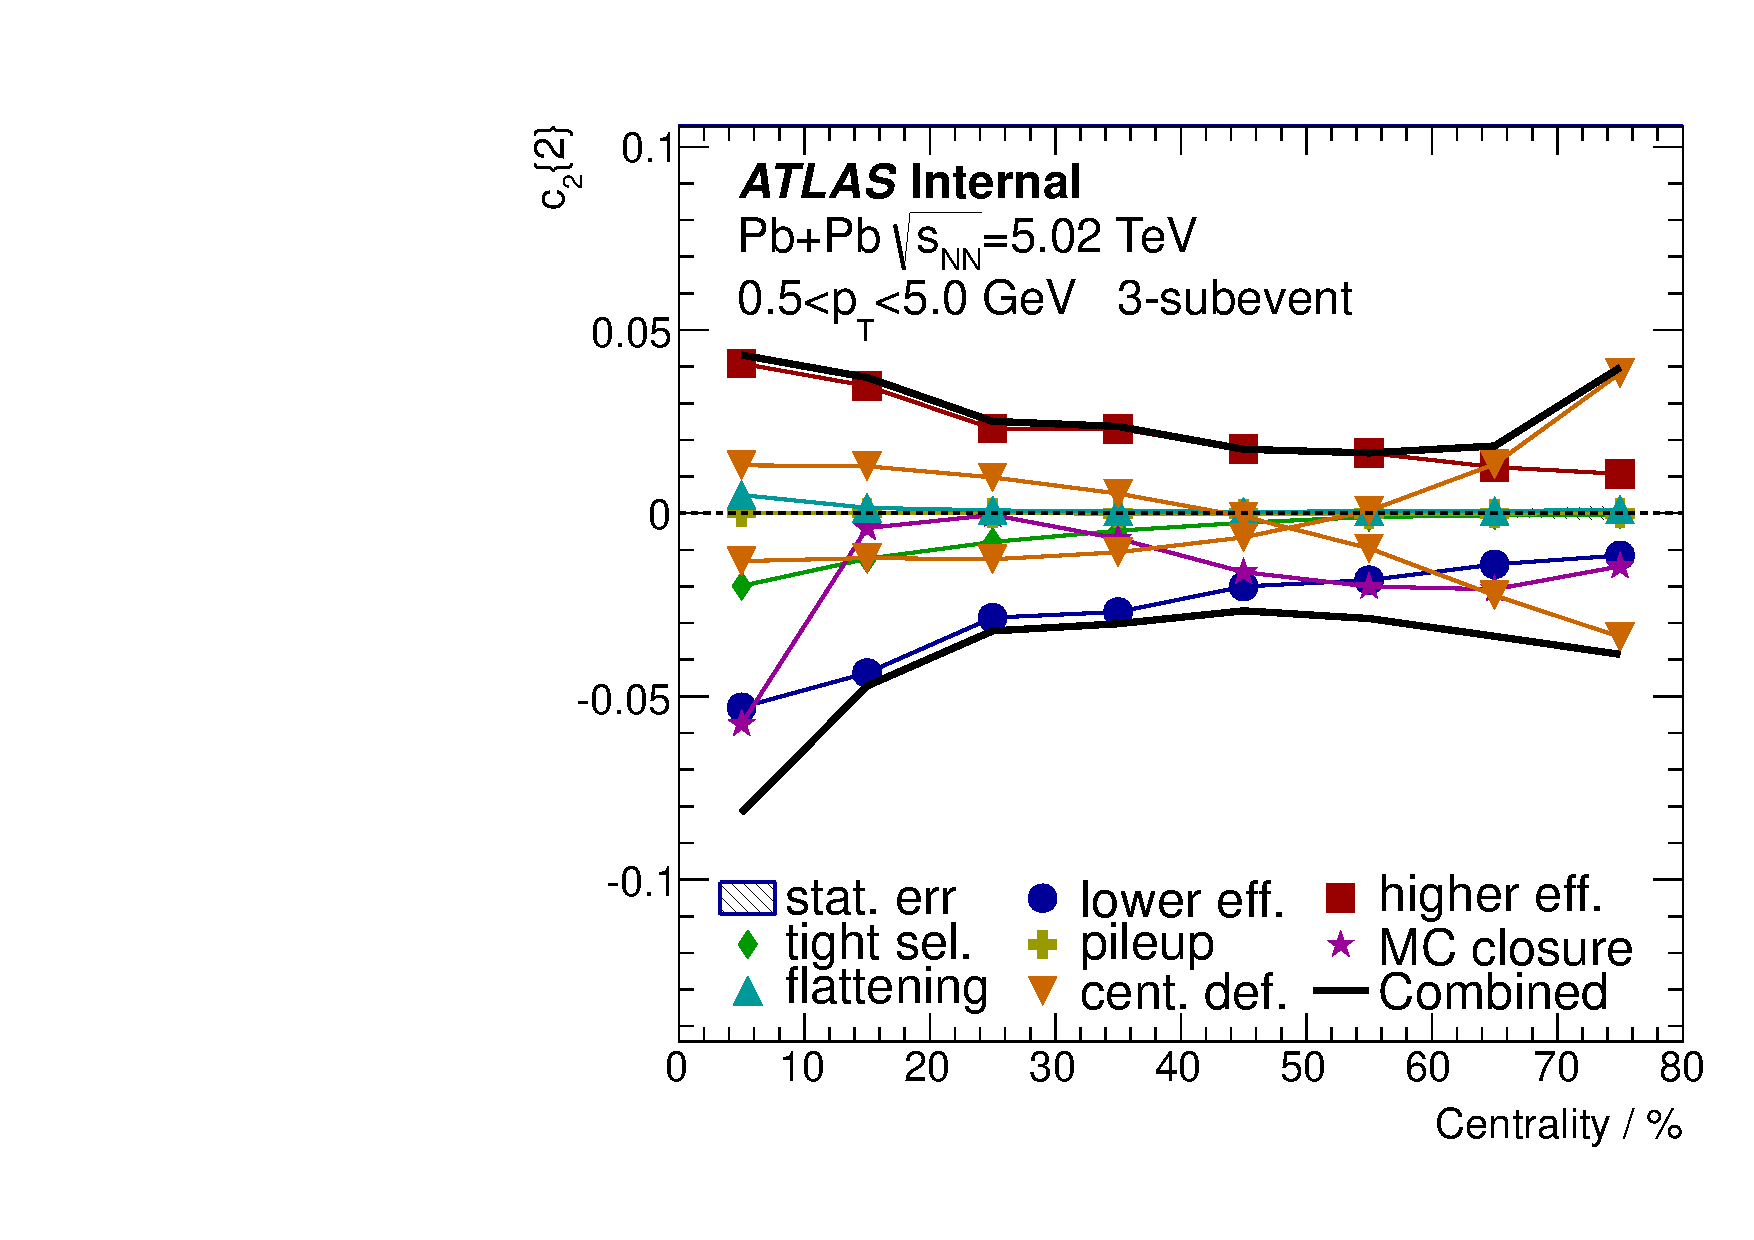
\includegraphics[width=.425\linewidth]{figs/sec_sys/summary/sys_c2_3sub_Har2_Pt0.pdf}
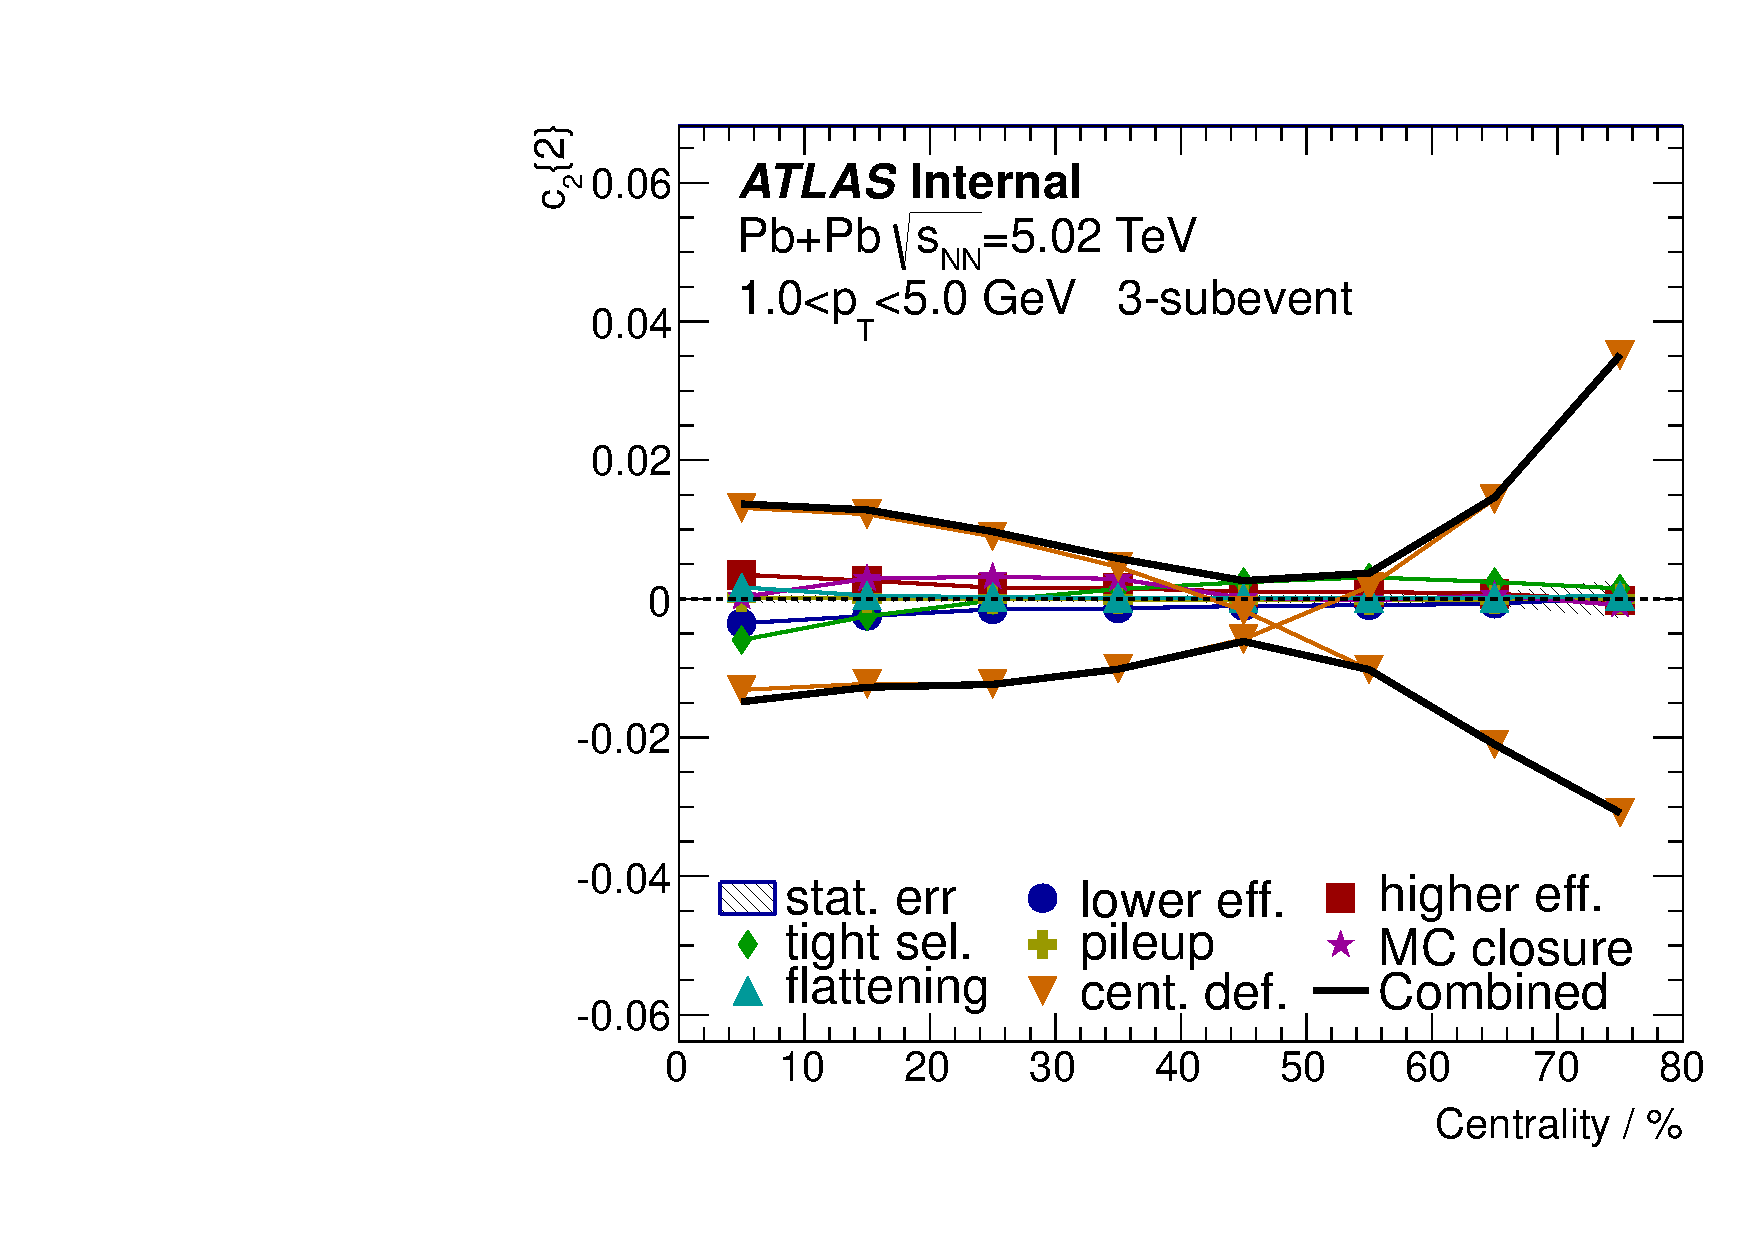
\includegraphics[width=.425\linewidth]{figs/sec_sys/summary/sys_c2_3sub_Har2_Pt1.pdf}
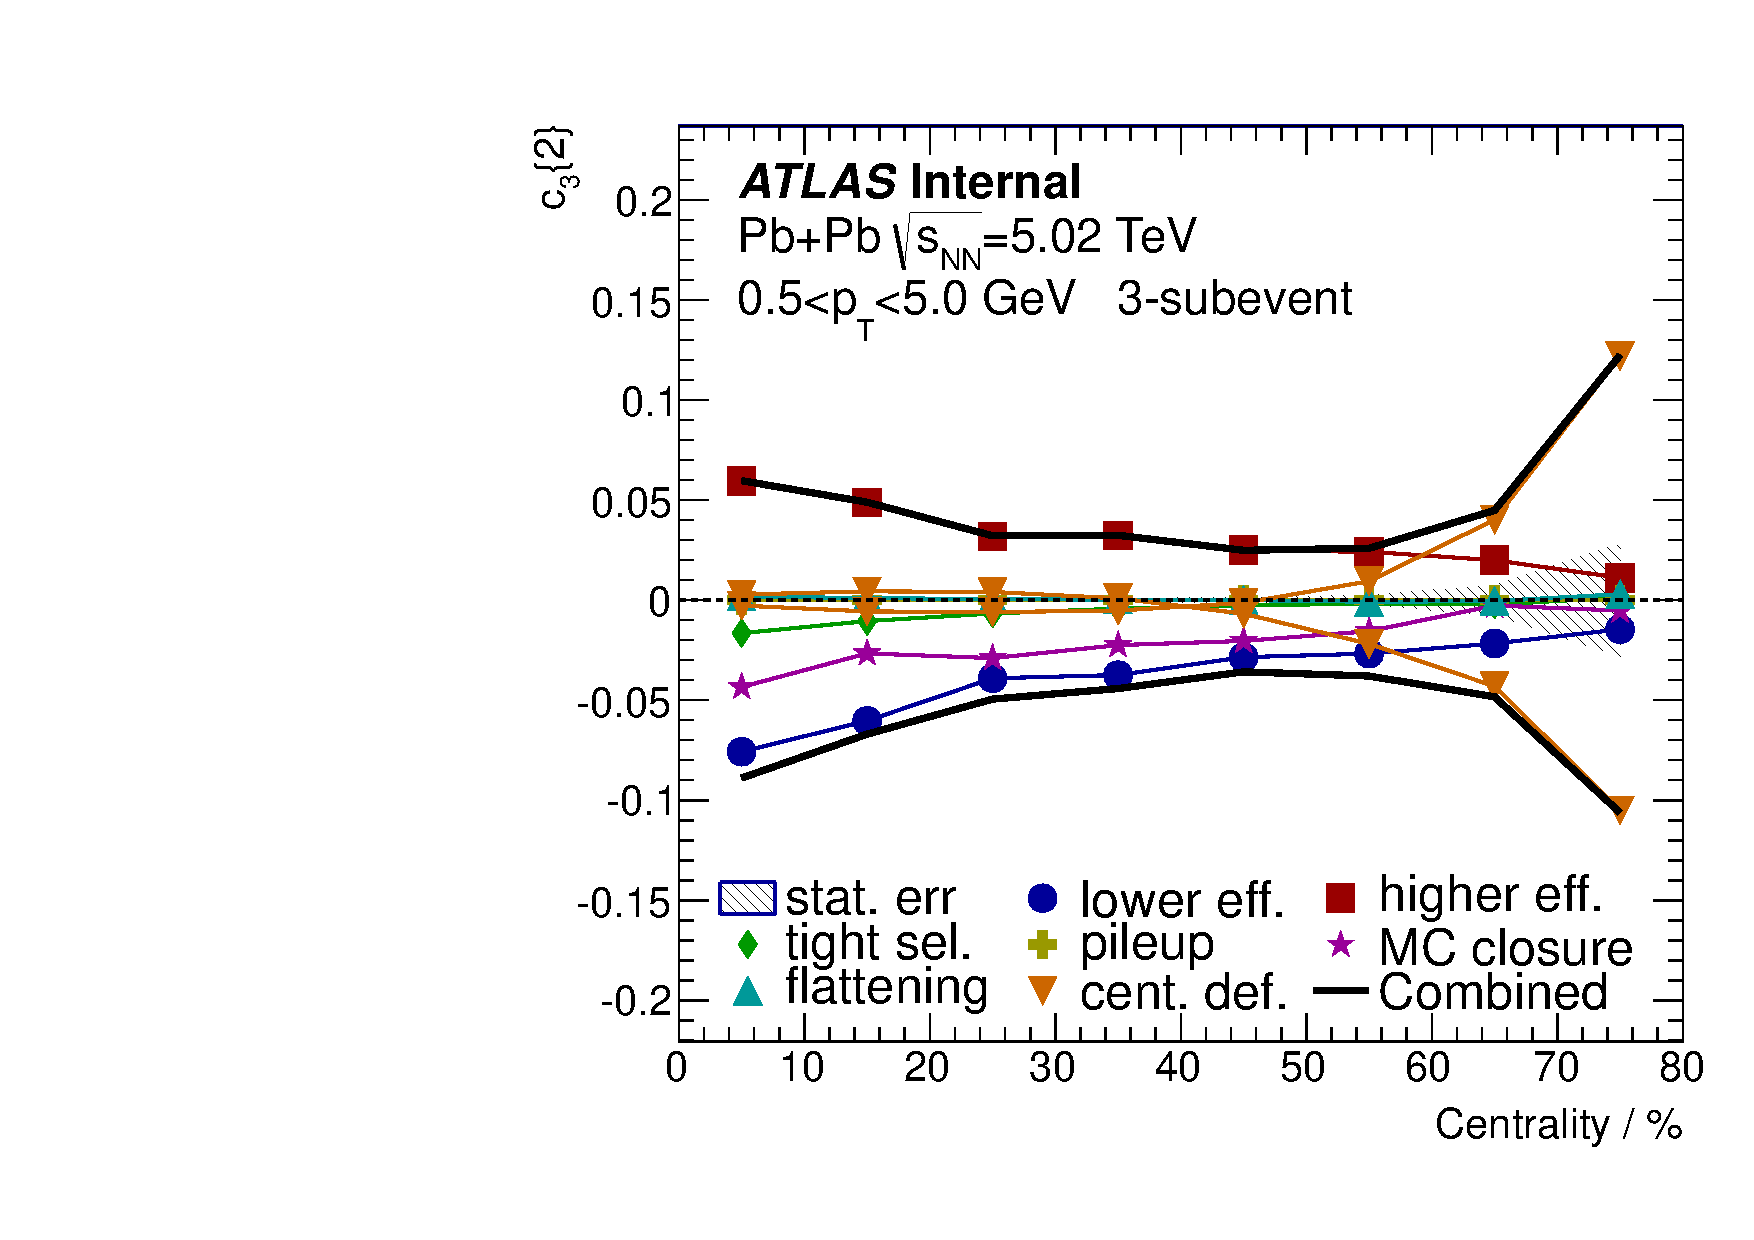
\includegraphics[width=.425\linewidth]{figs/sec_sys/summary/sys_c2_3sub_Har3_Pt0.pdf}
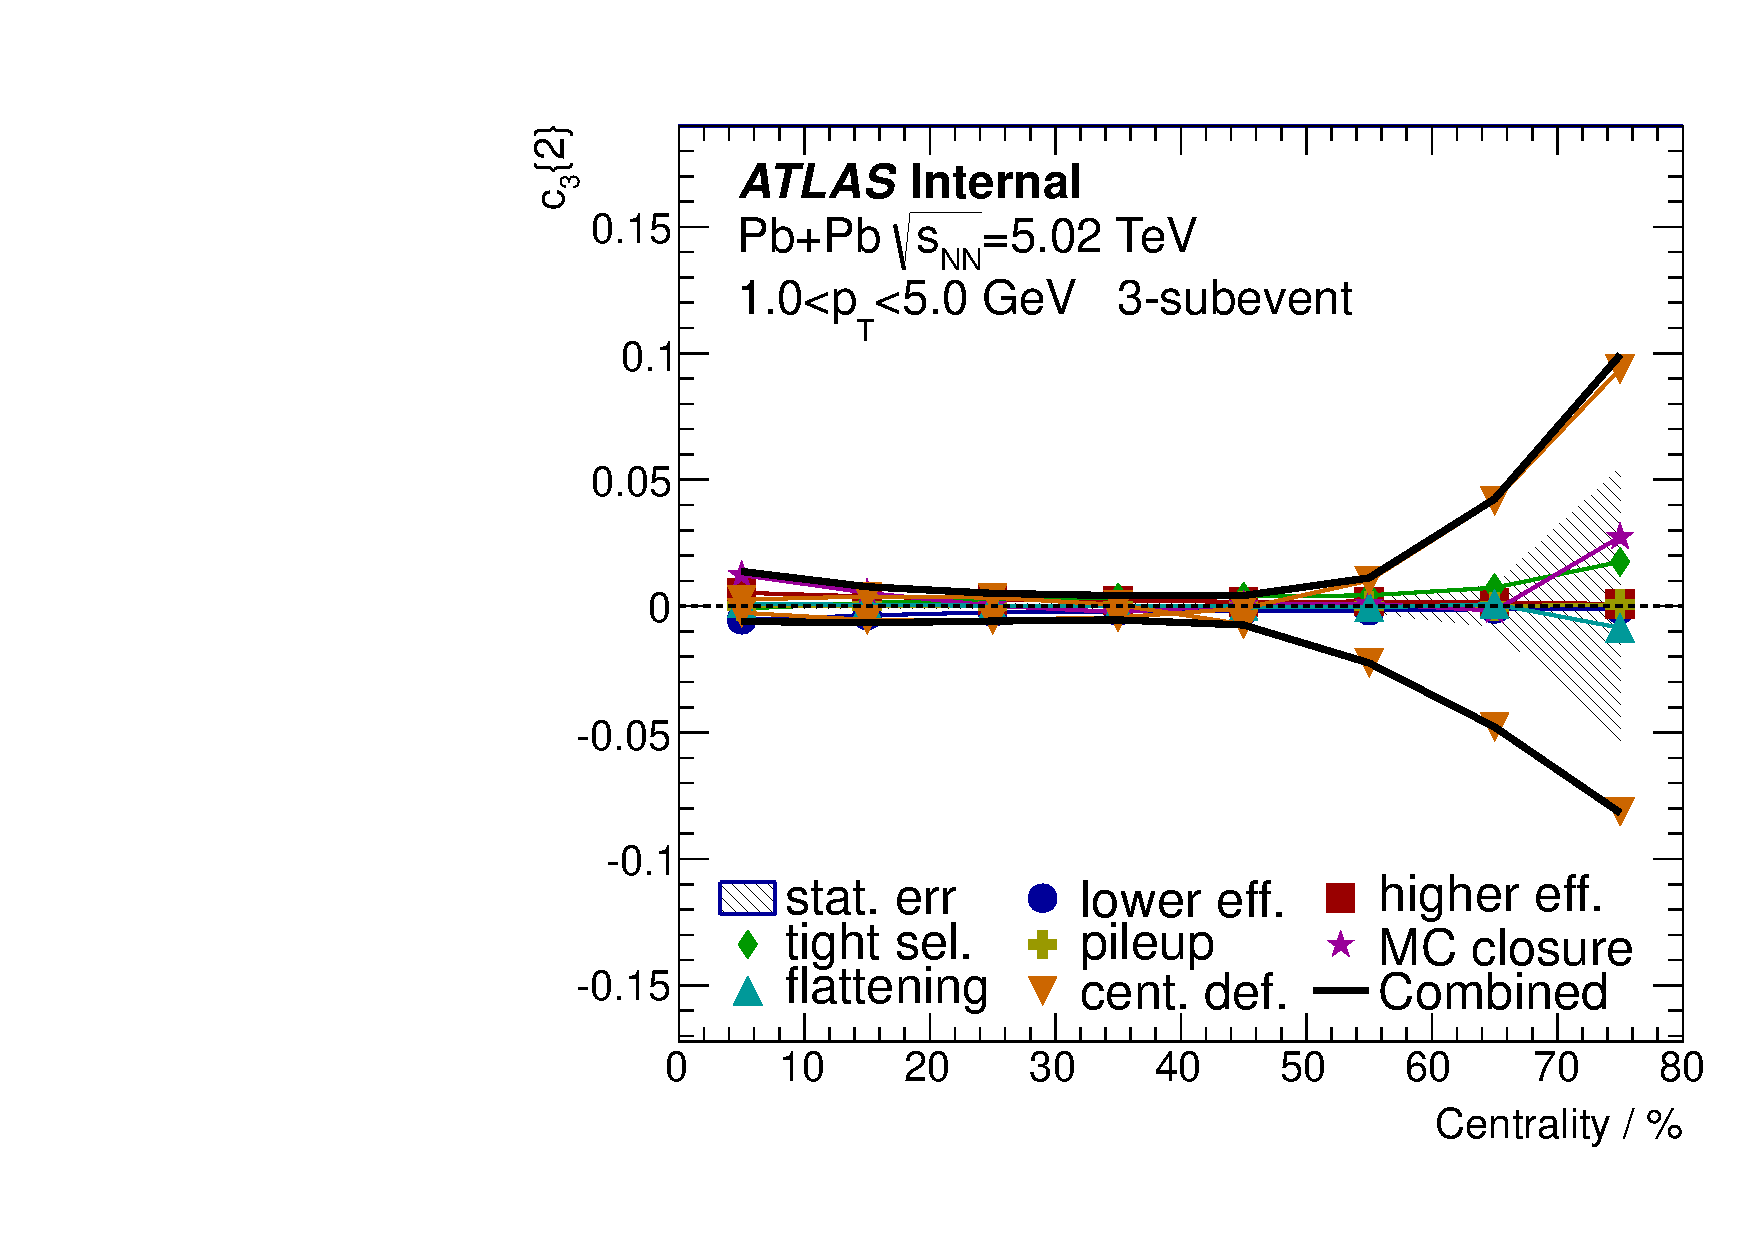
\includegraphics[width=.425\linewidth]{figs/sec_sys/summary/sys_c2_3sub_Har3_Pt1.pdf}
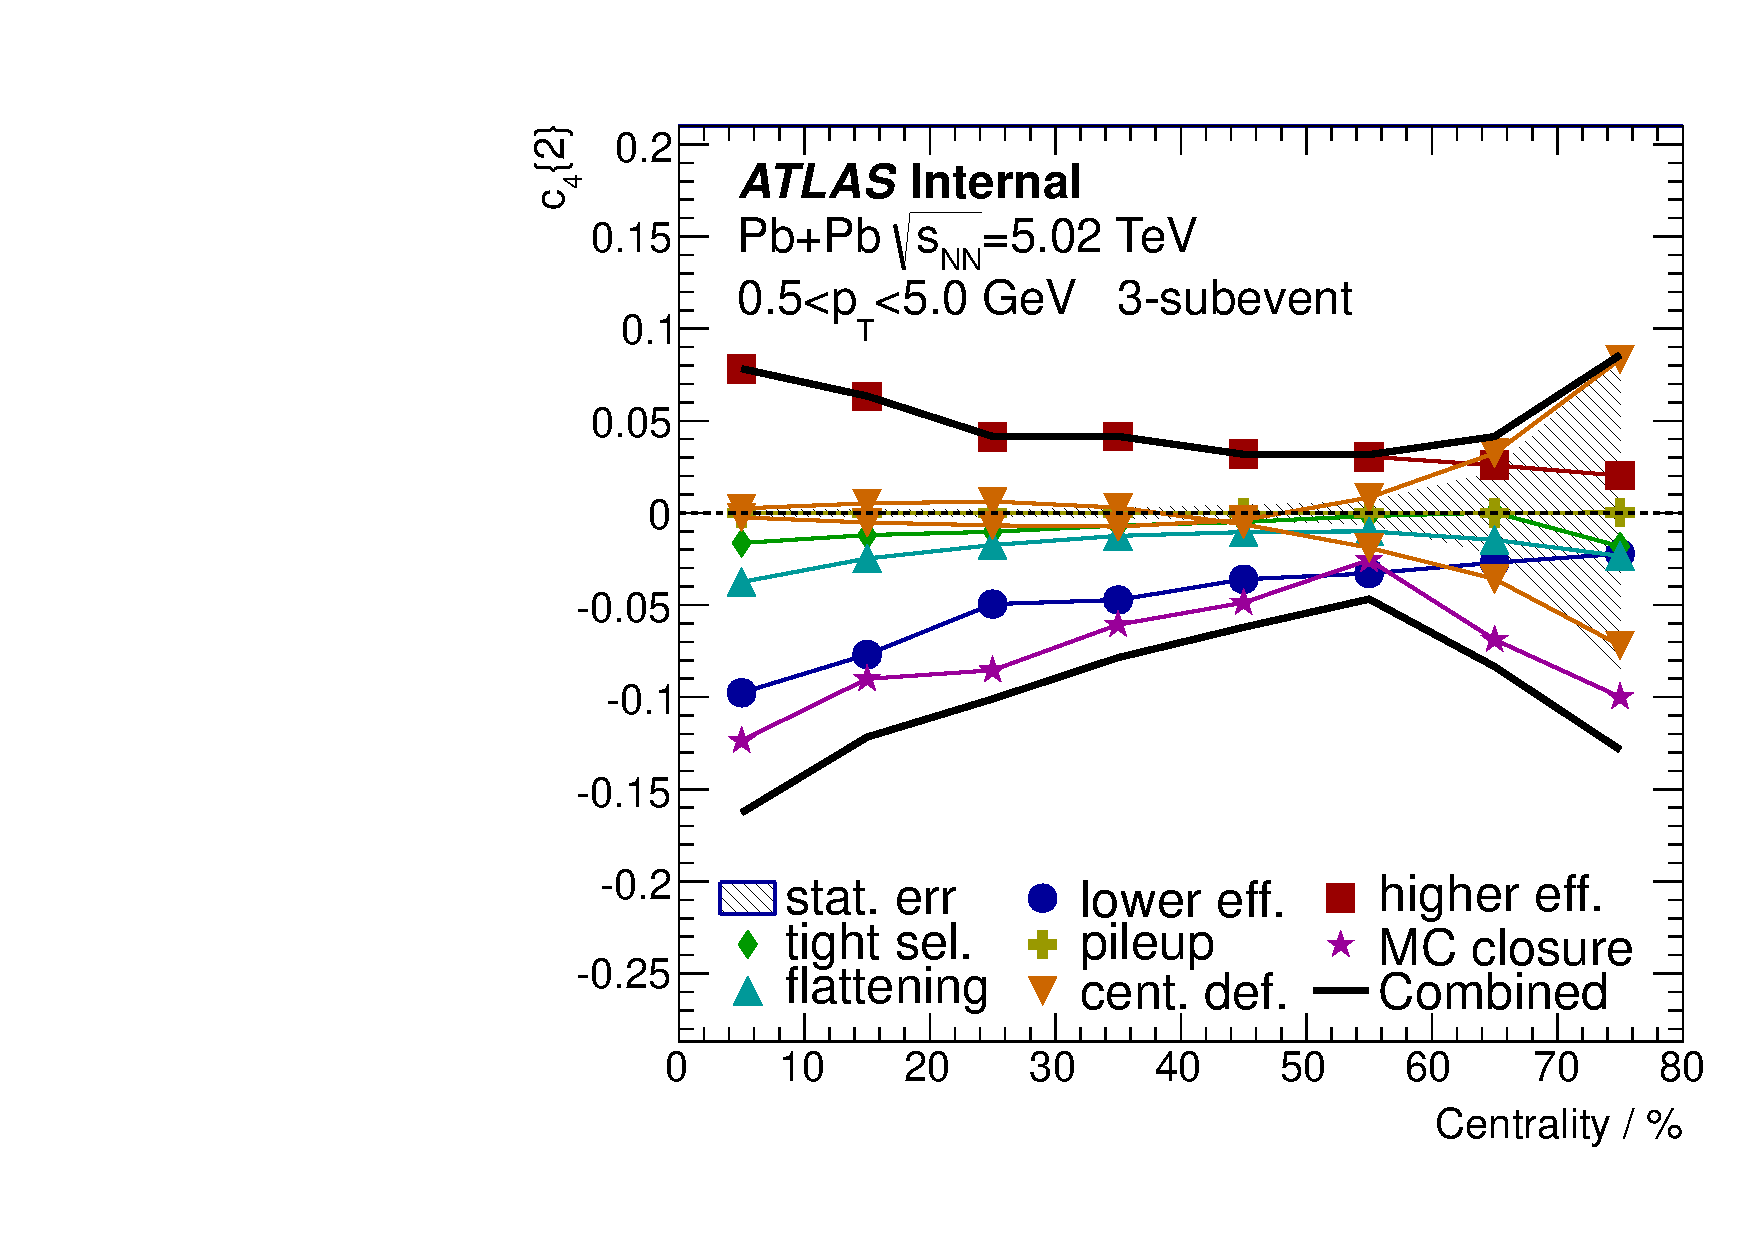
\includegraphics[width=.425\linewidth]{figs/sec_sys/summary/sys_c2_3sub_Har4_Pt0.pdf}
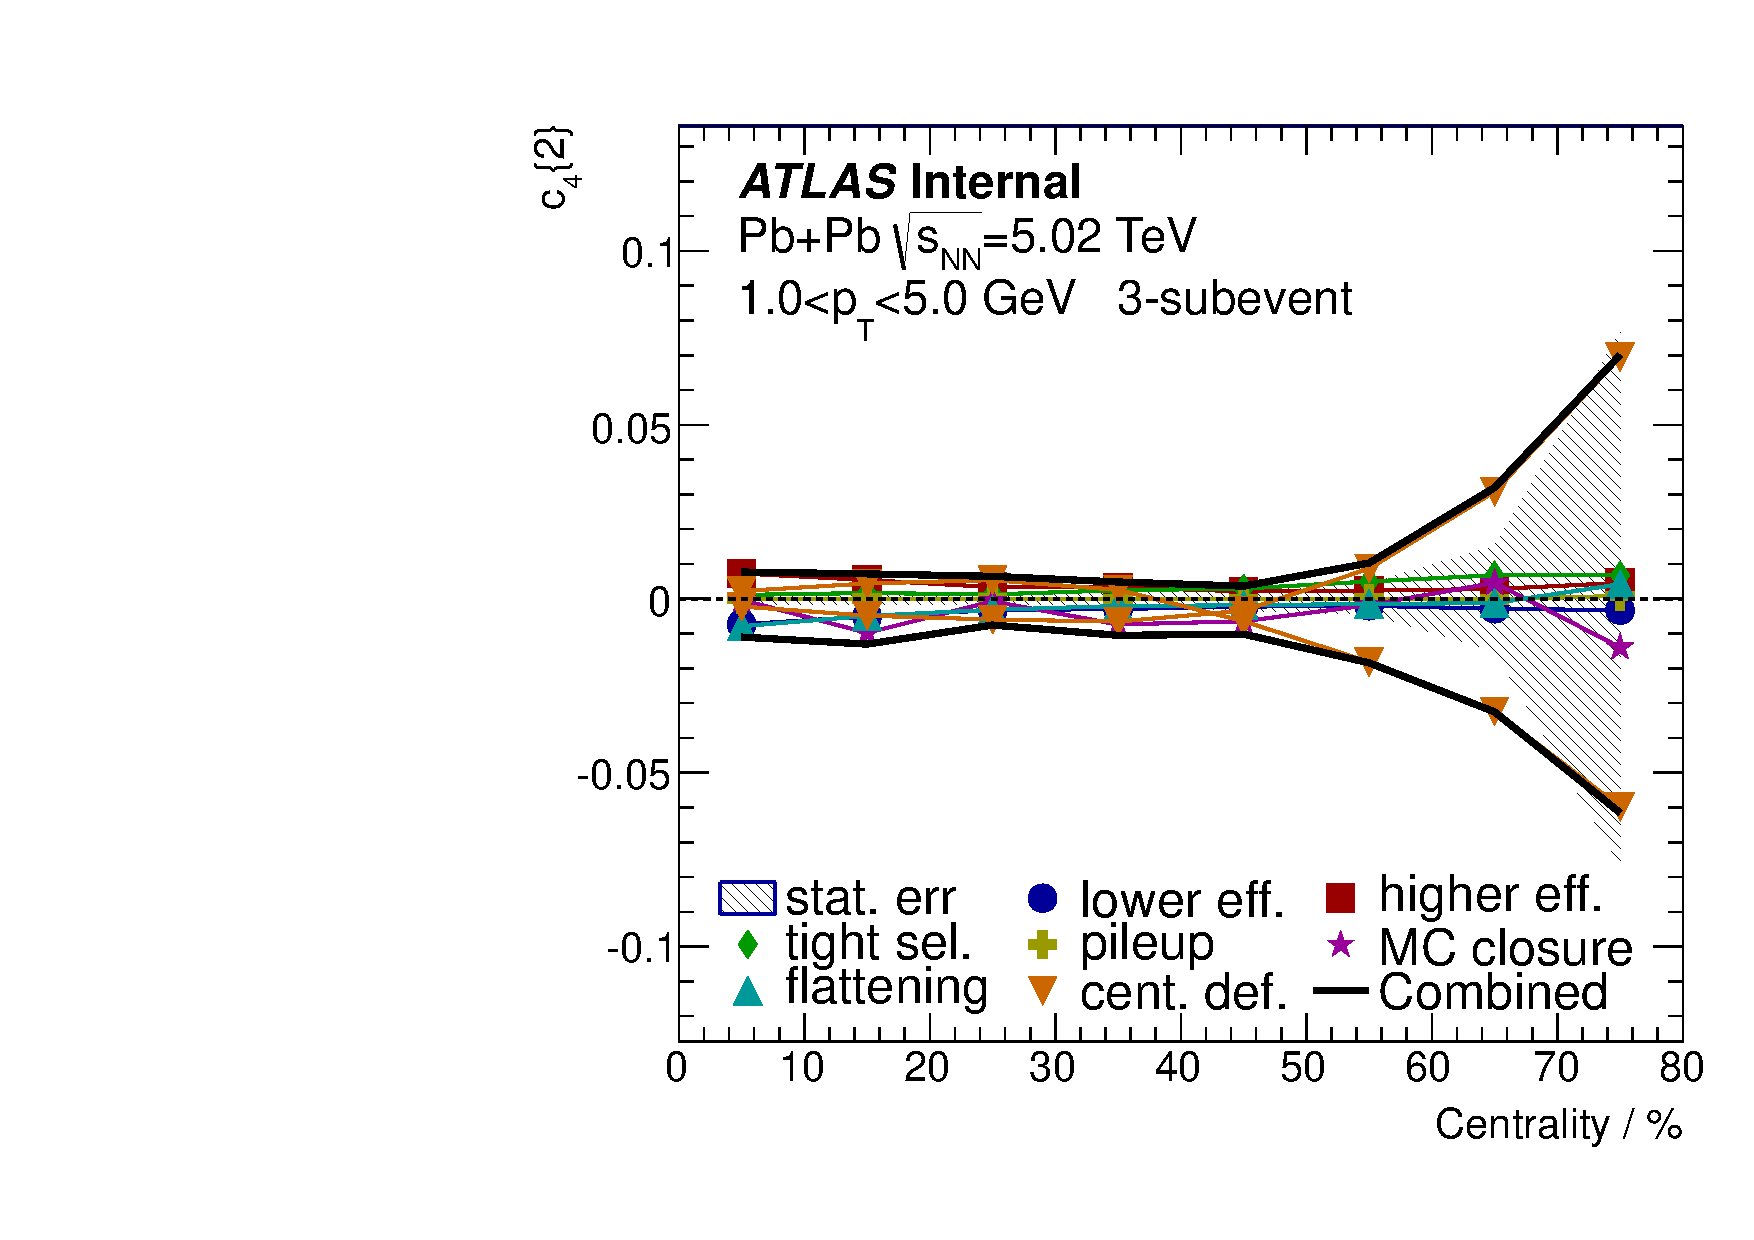
\includegraphics[width=.425\linewidth]{figs/sec_sys/summary/sys_c2_3sub_Har4_Pt1.pdf}
\caption{Breakdown of systematics for 2-particle cumulant $c_n\{2\}$ using 3-subevent method, with low (left) and high (right) $p_\text{T}$ ranges. Different rows are for different harmonics.}
\label{fig:apdx_sys_c2_3sub}
\end{figure}

\begin{figure}[H]
\centering
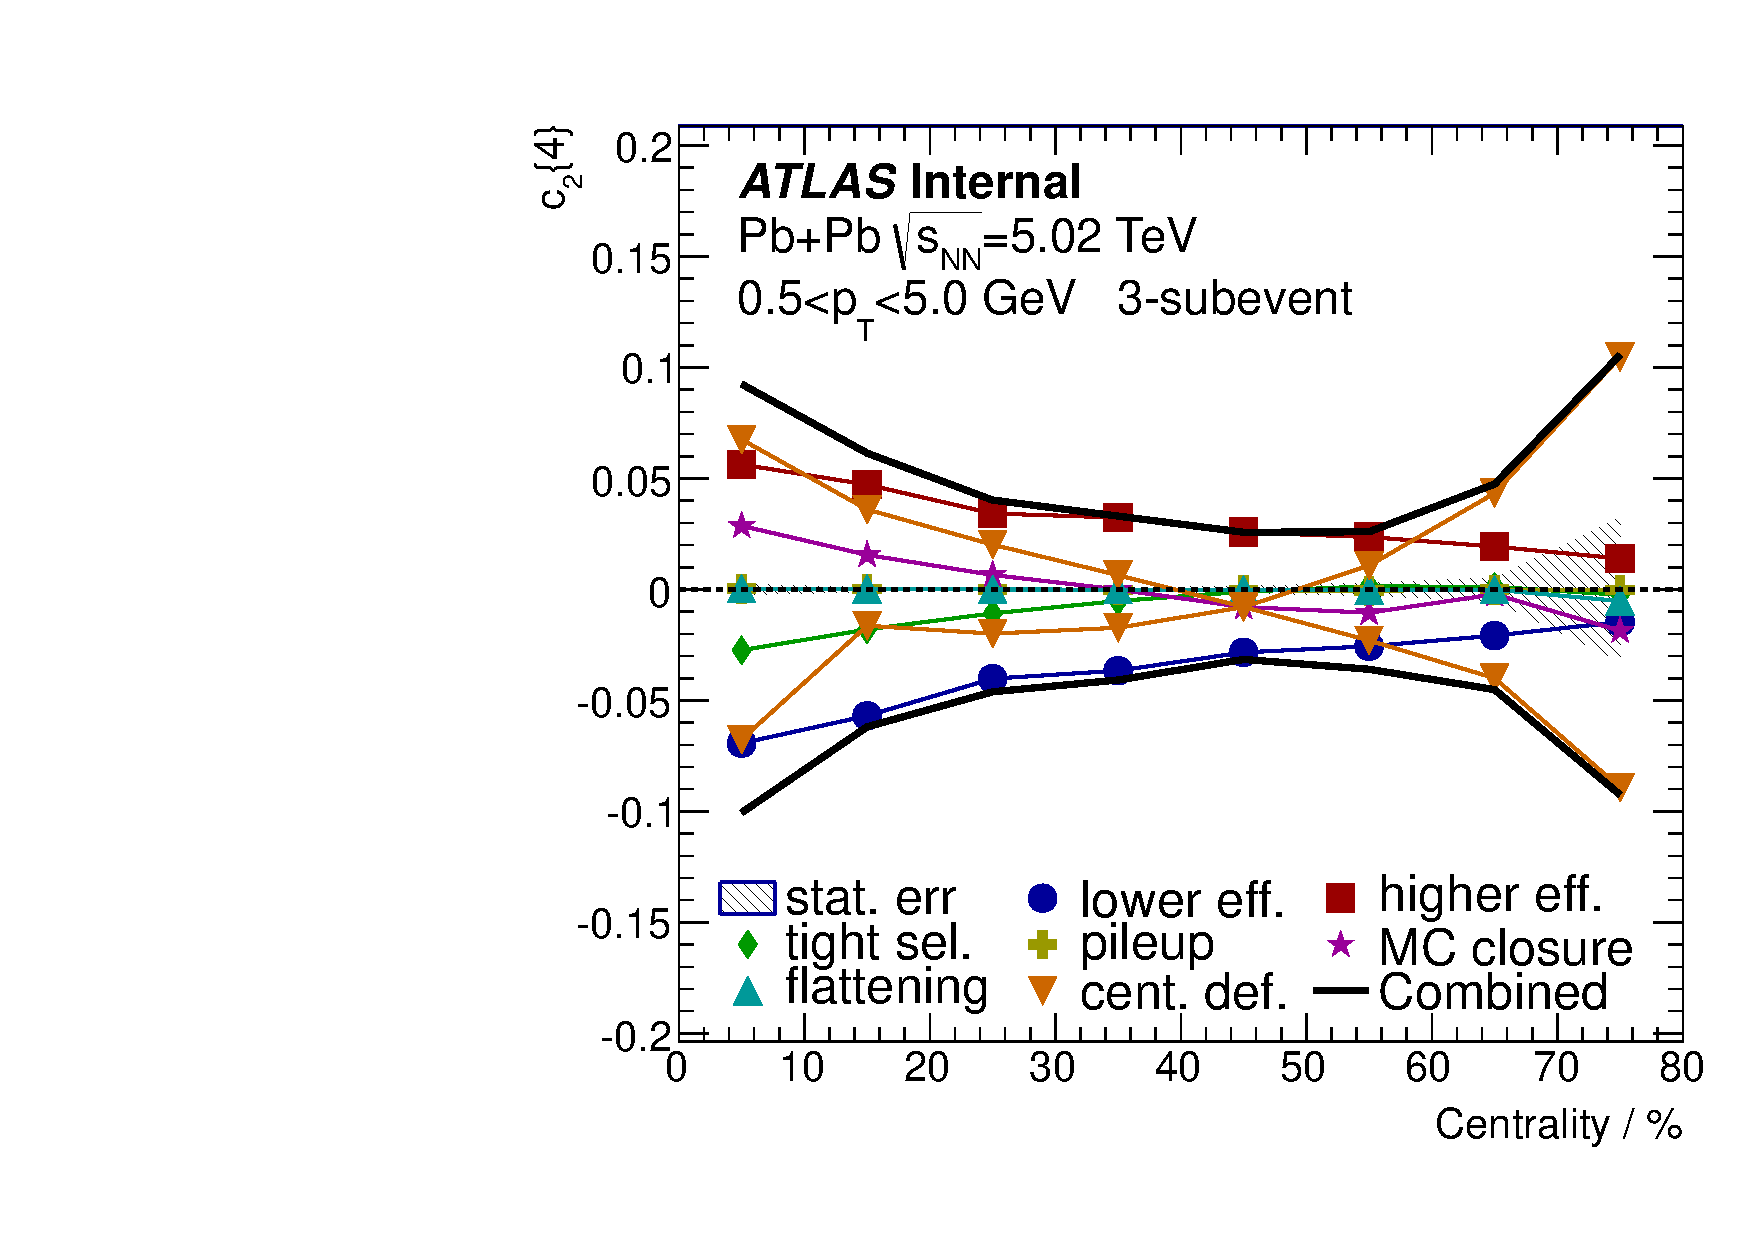
\includegraphics[width=.425\linewidth]{figs/sec_sys/summary/sys_c4_3sub_Har2_Pt0.pdf}
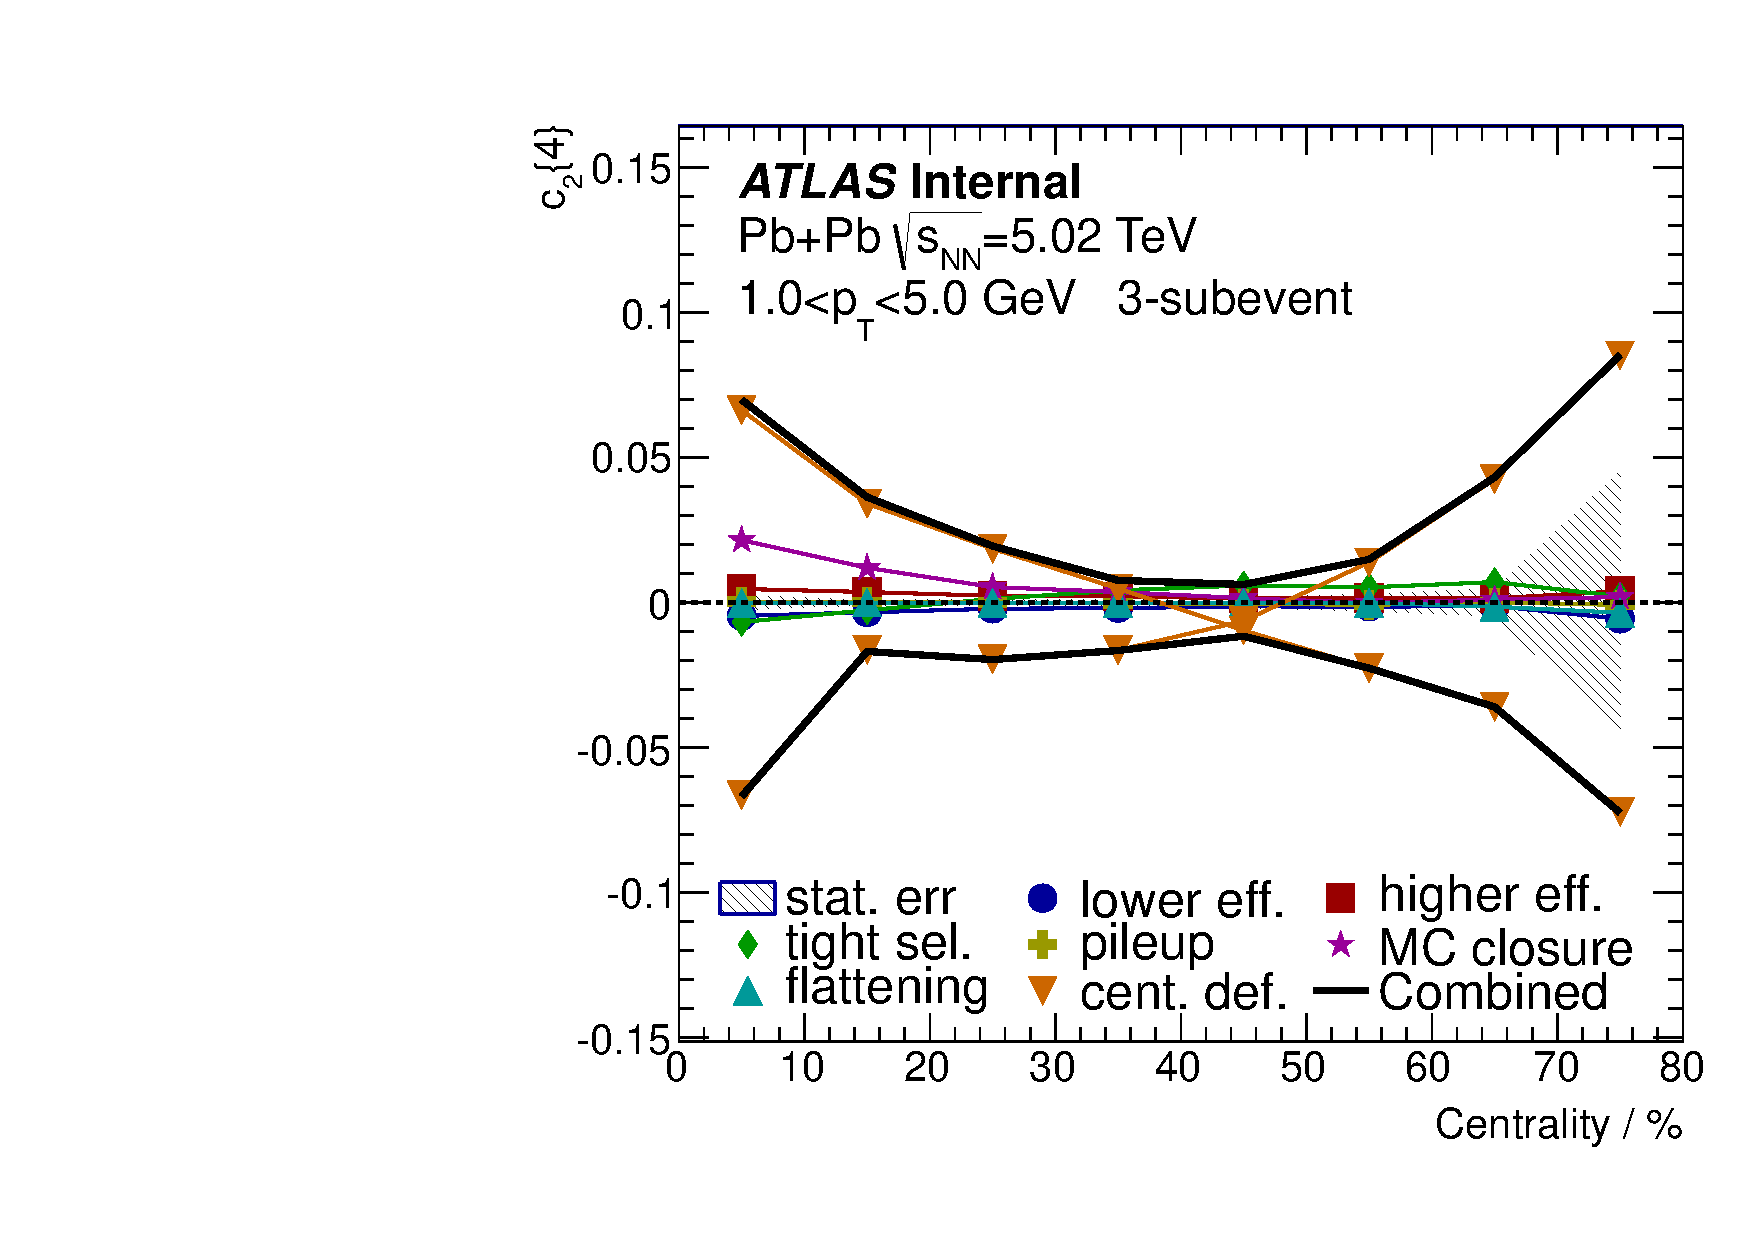
\includegraphics[width=.425\linewidth]{figs/sec_sys/summary/sys_c4_3sub_Har2_Pt1.pdf}
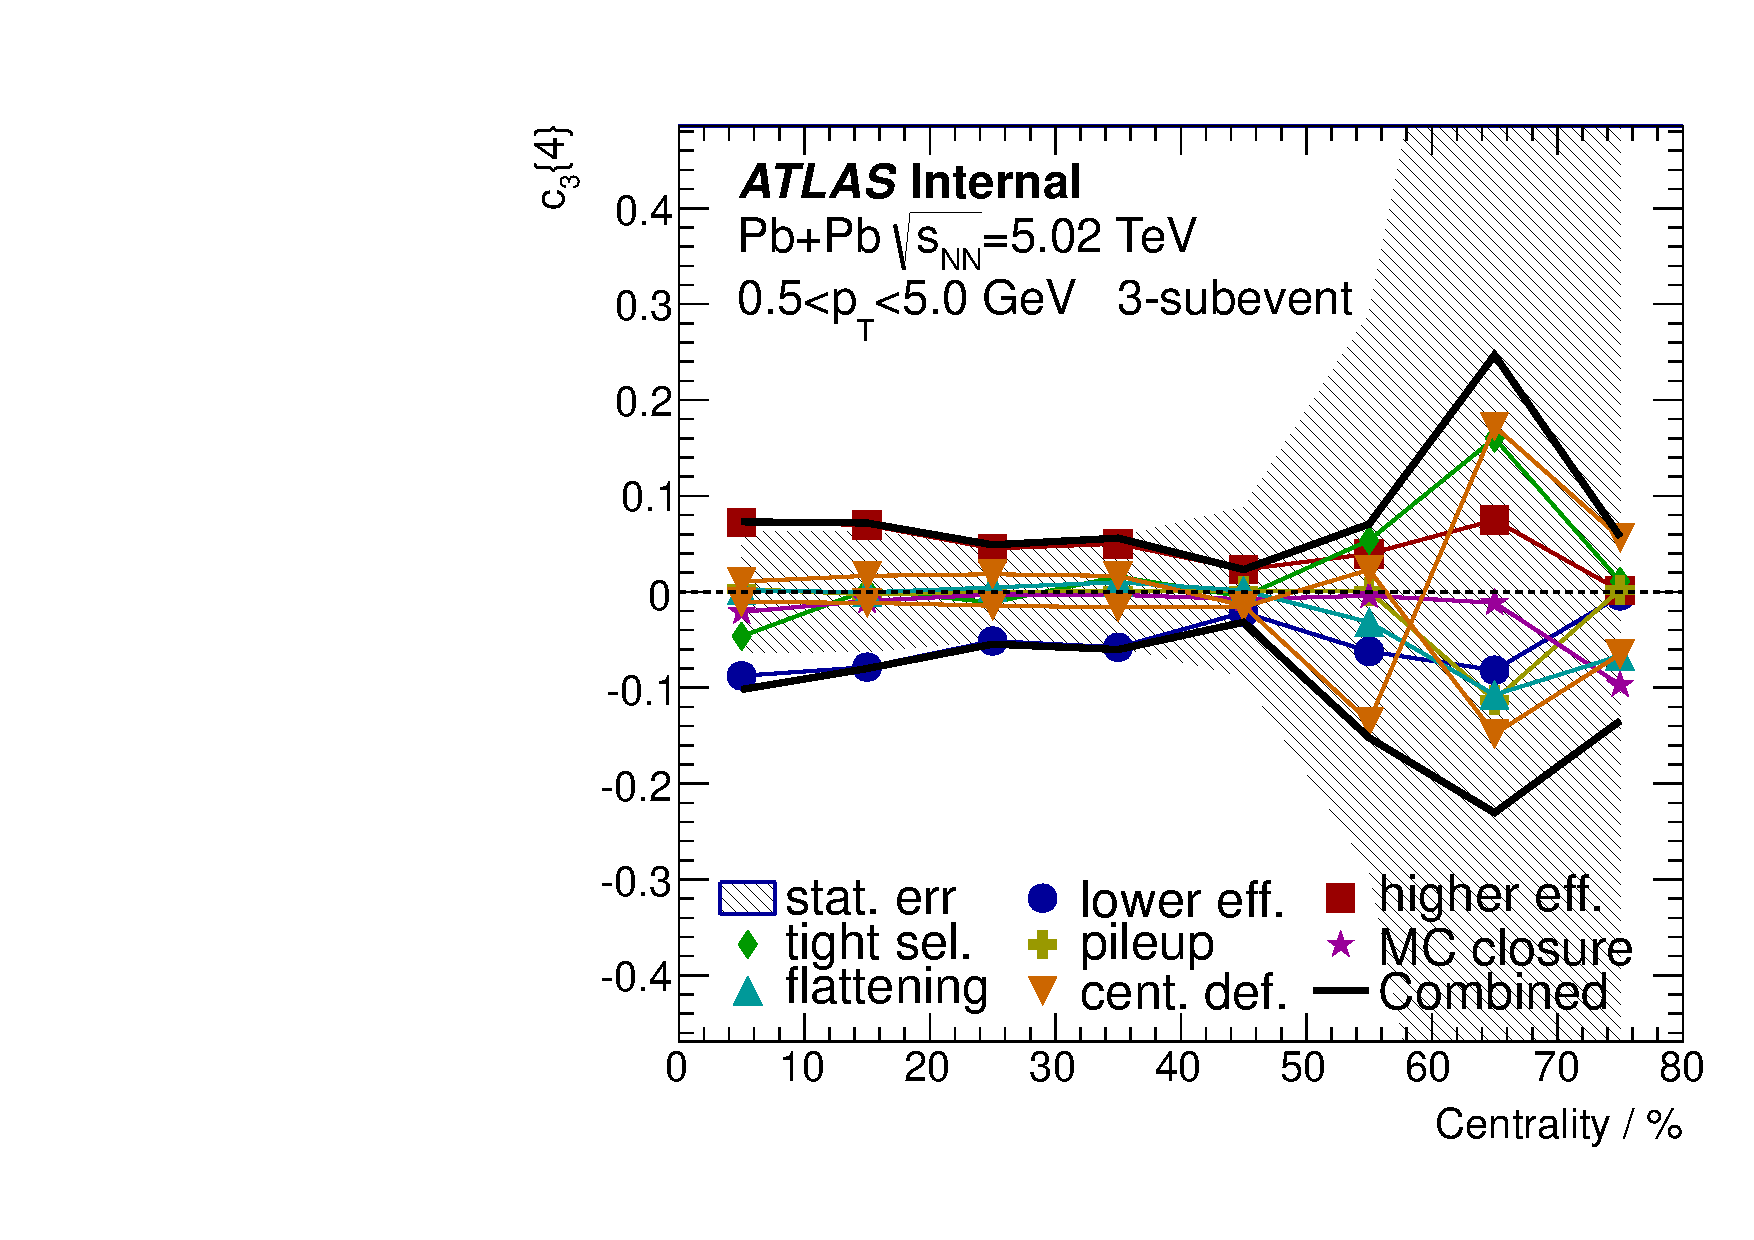
\includegraphics[width=.425\linewidth]{figs/sec_sys/summary/sys_c4_3sub_Har3_Pt0.pdf}
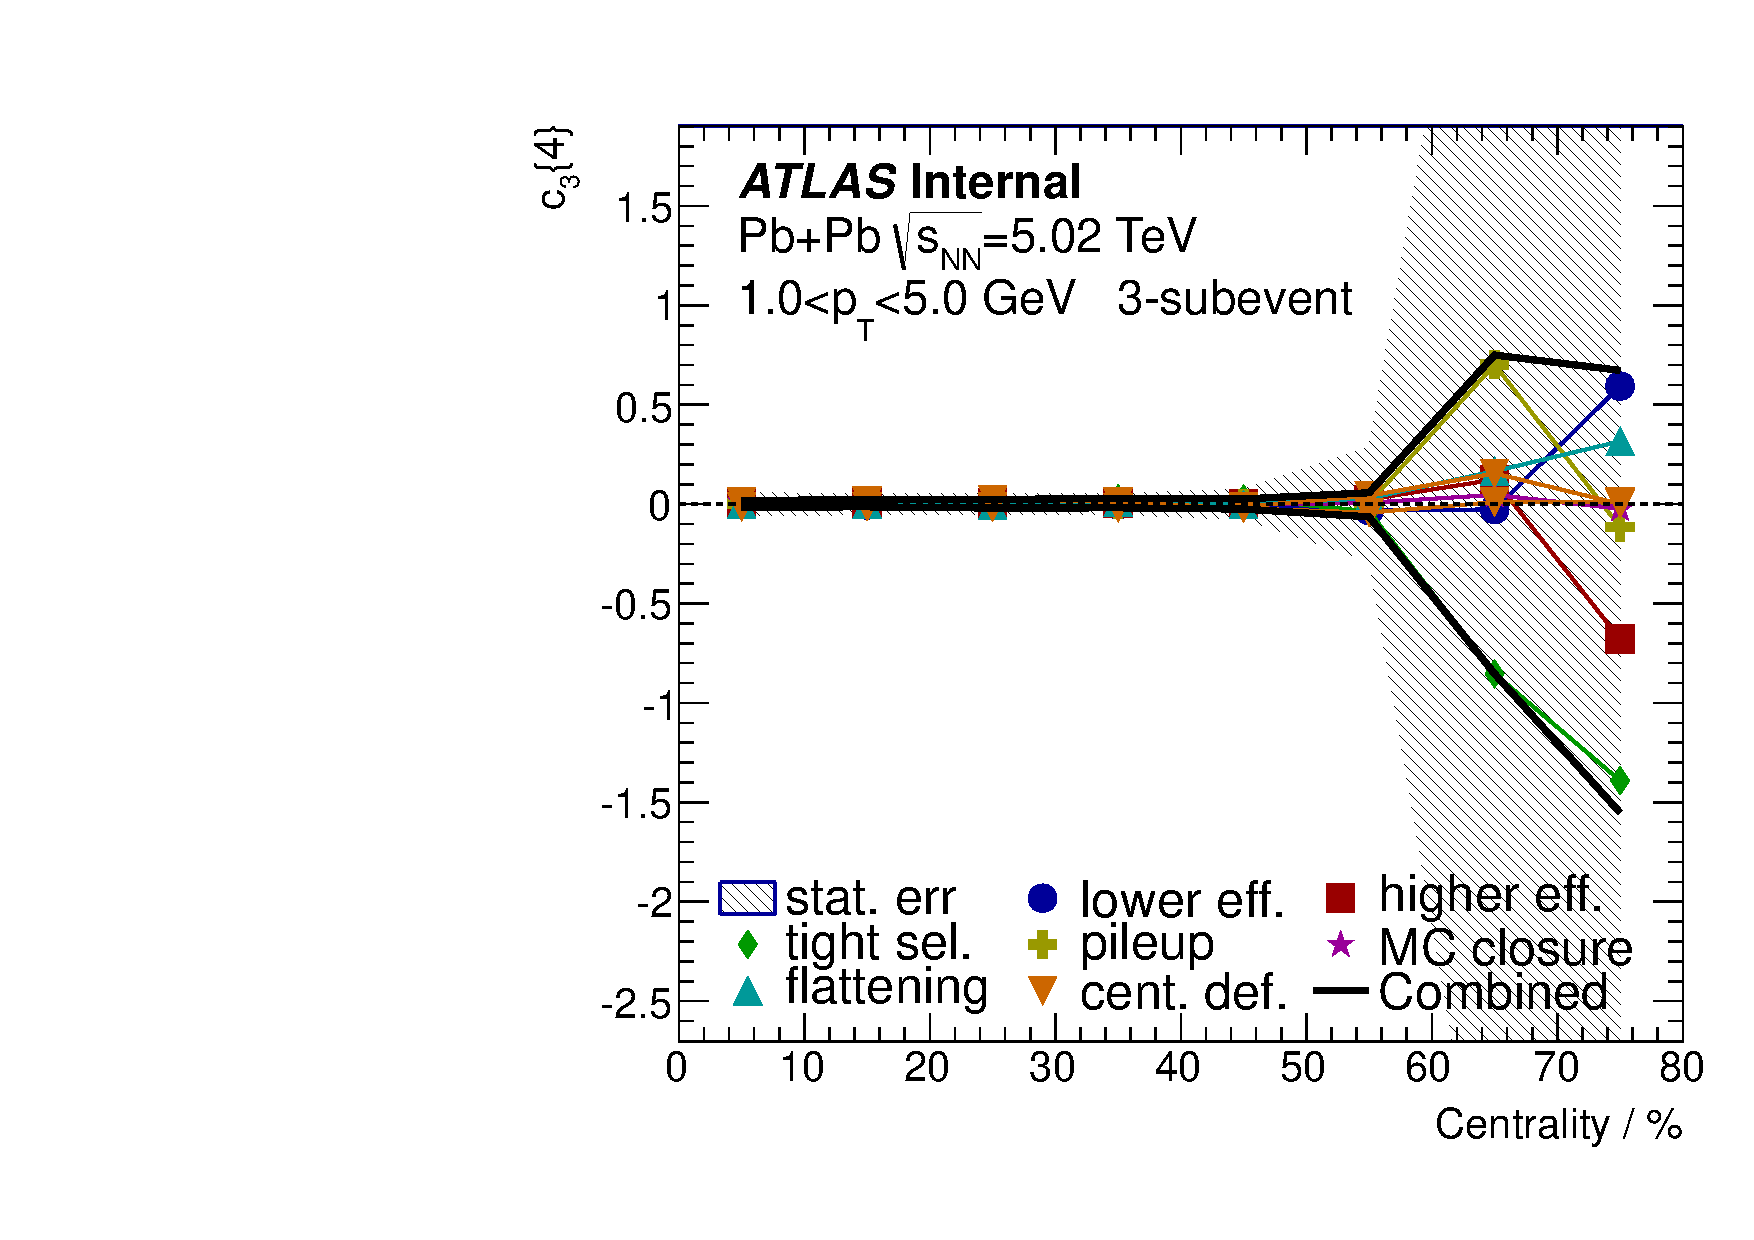
\includegraphics[width=.425\linewidth]{figs/sec_sys/summary/sys_c4_3sub_Har3_Pt1.pdf}
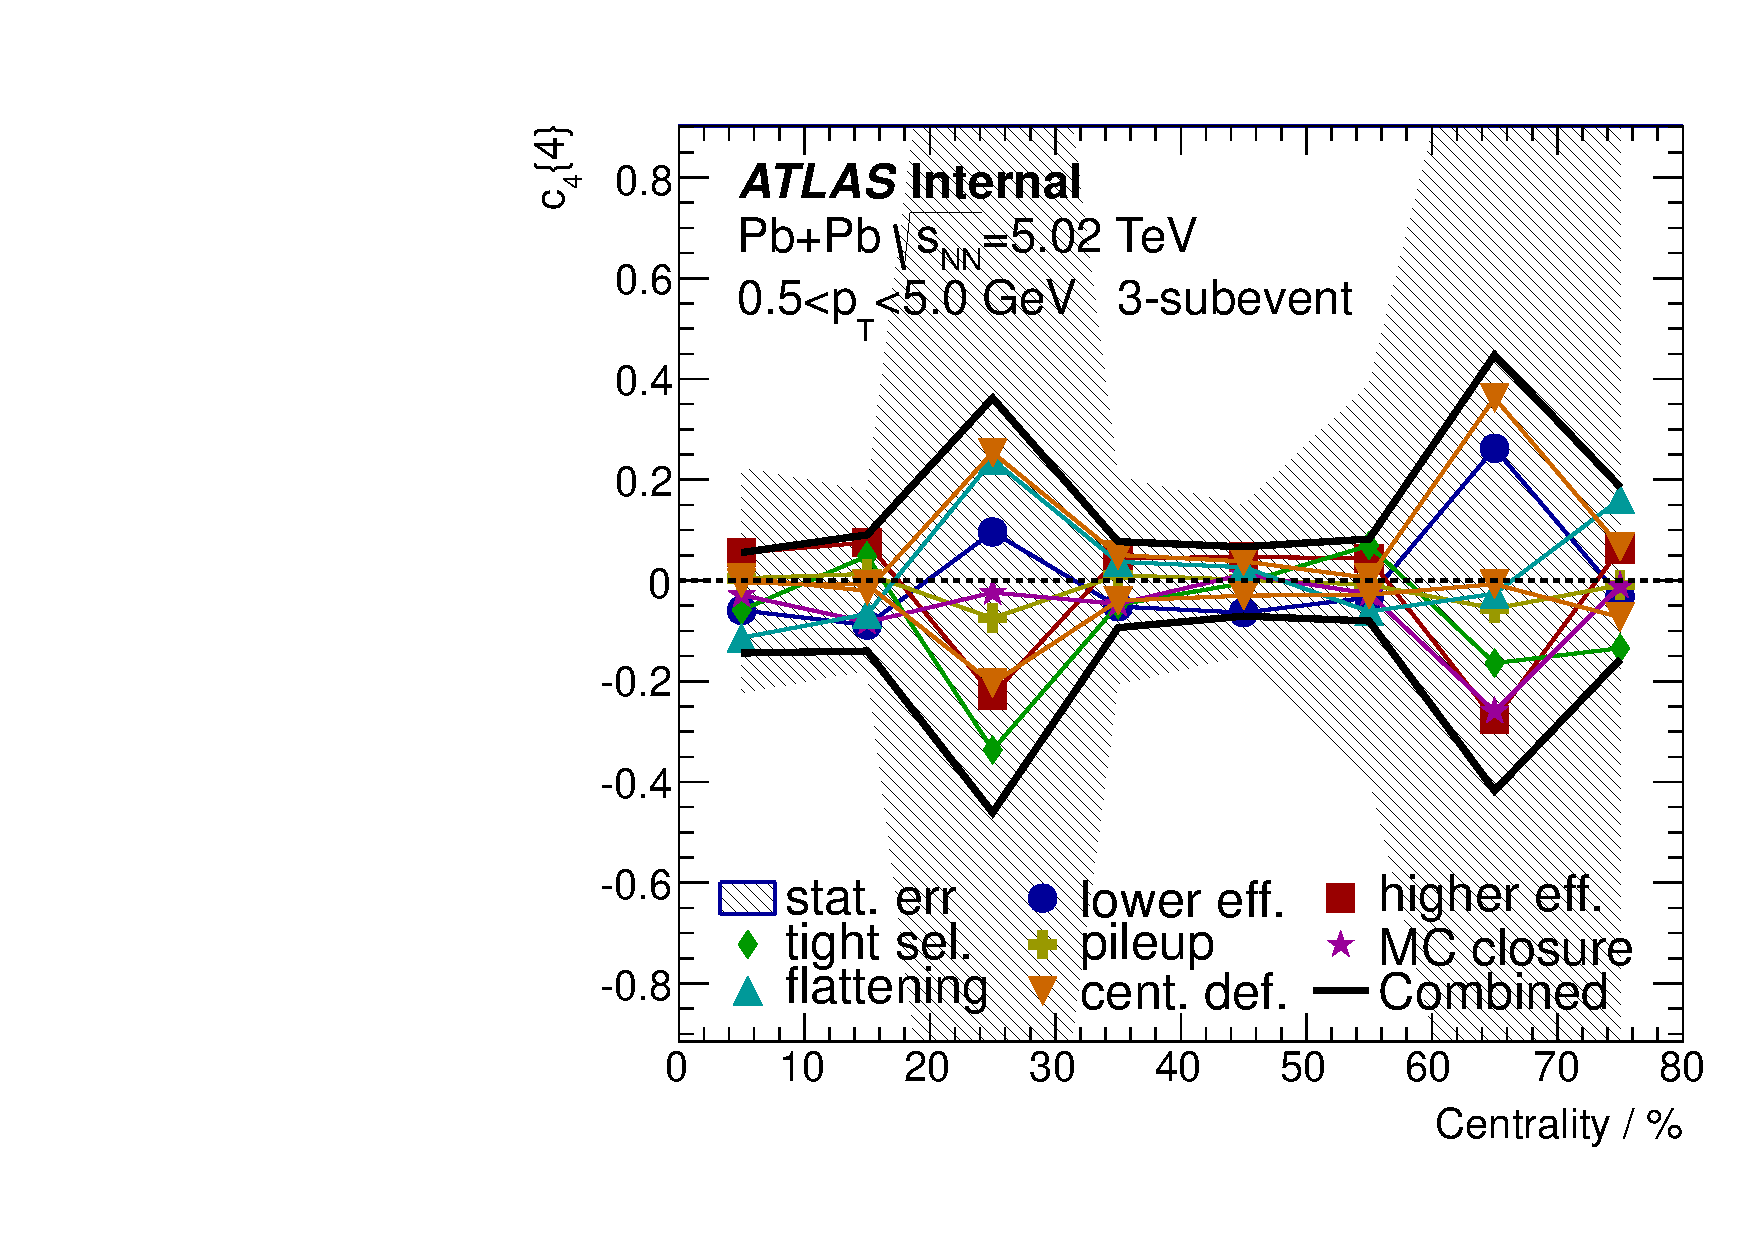
\includegraphics[width=.425\linewidth]{figs/sec_sys/summary/sys_c4_3sub_Har4_Pt0.pdf}
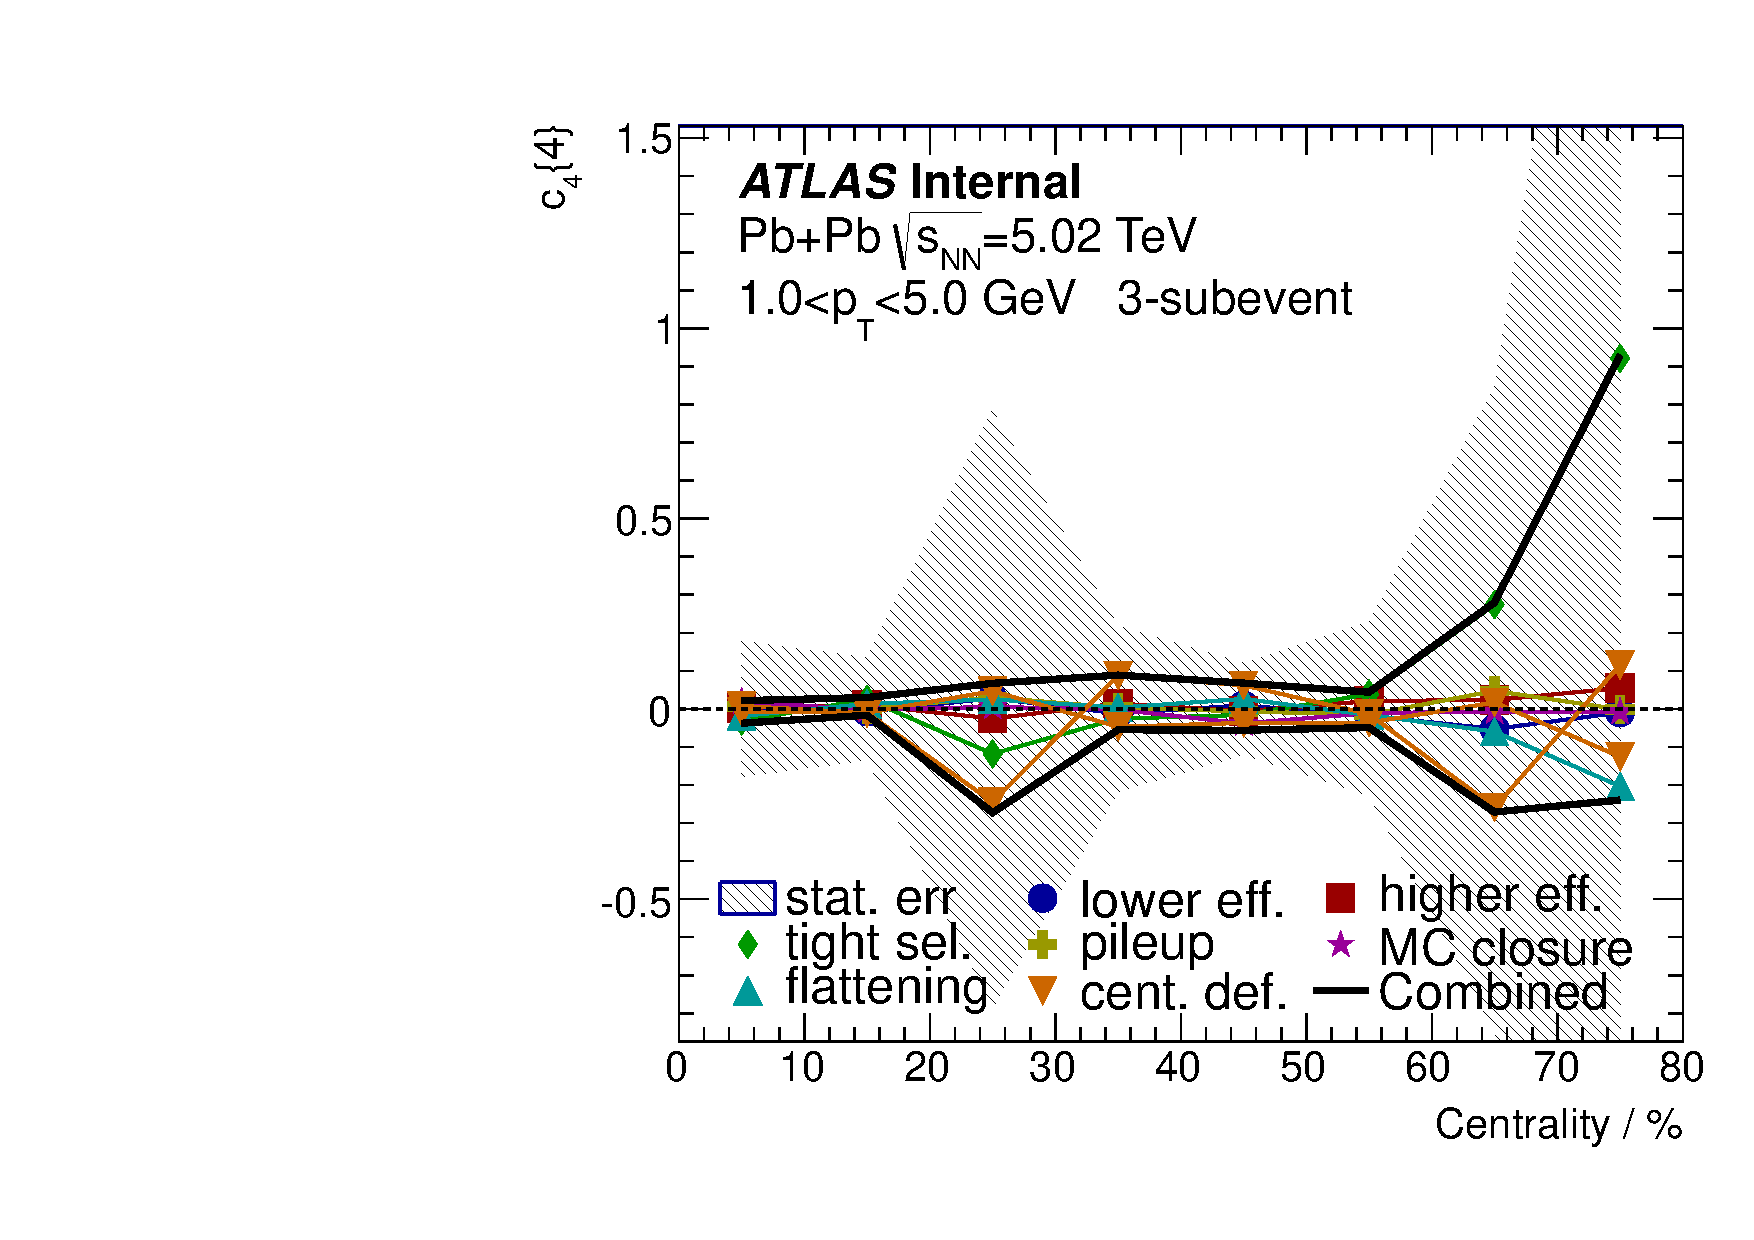
\includegraphics[width=.425\linewidth]{figs/sec_sys/summary/sys_c4_3sub_Har4_Pt1.pdf}
\caption{Breakdown of systematics for 4-particle cumulant $c_n\{4\}$ using 3-subevent method, with low (left) and high (right) $p_\text{T}$ ranges. Different rows are for different harmonics.}
\label{fig:apdx_sys_c4_3sub}
\end{figure}

\begin{figure}[H]
\centering
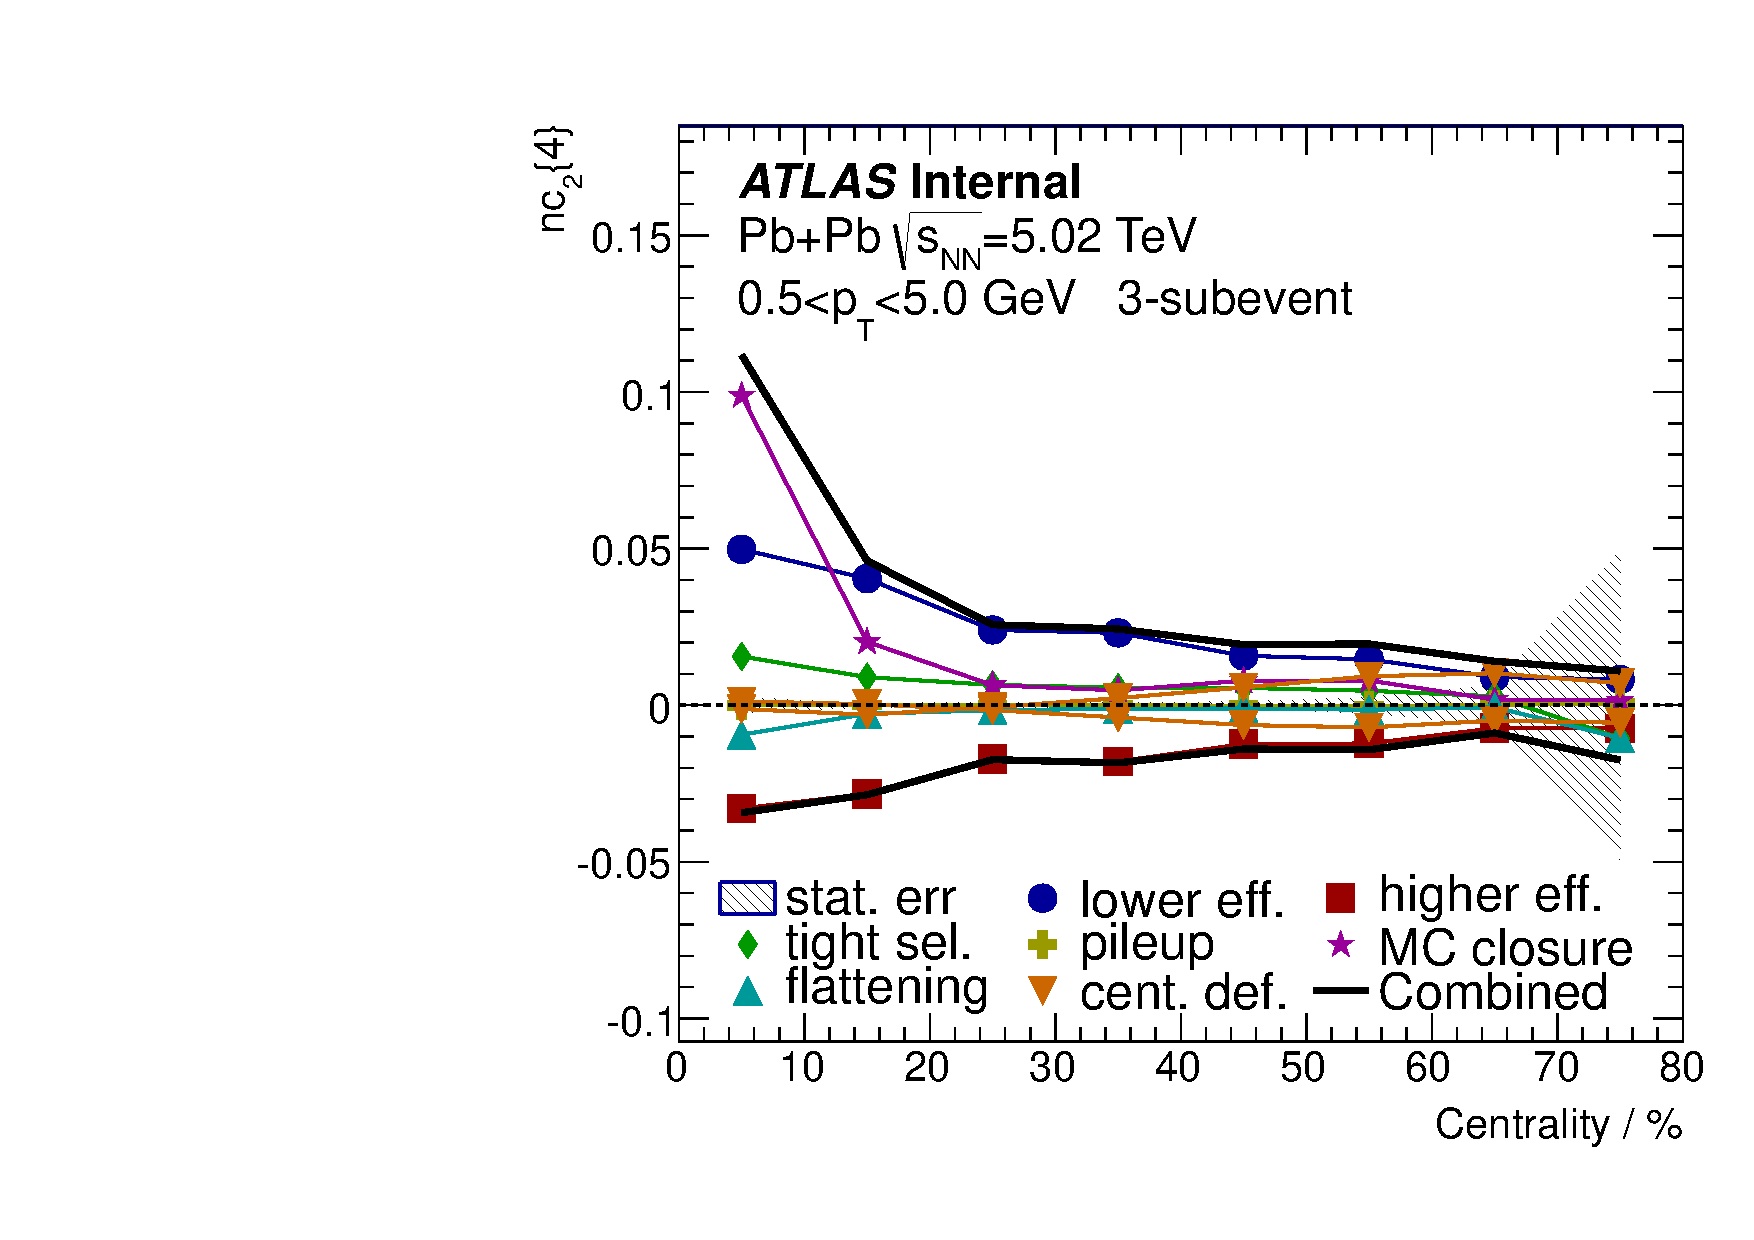
\includegraphics[width=.425\linewidth]{figs/sec_sys/summary/sys_nc4_3sub_Har2_Pt0.pdf}
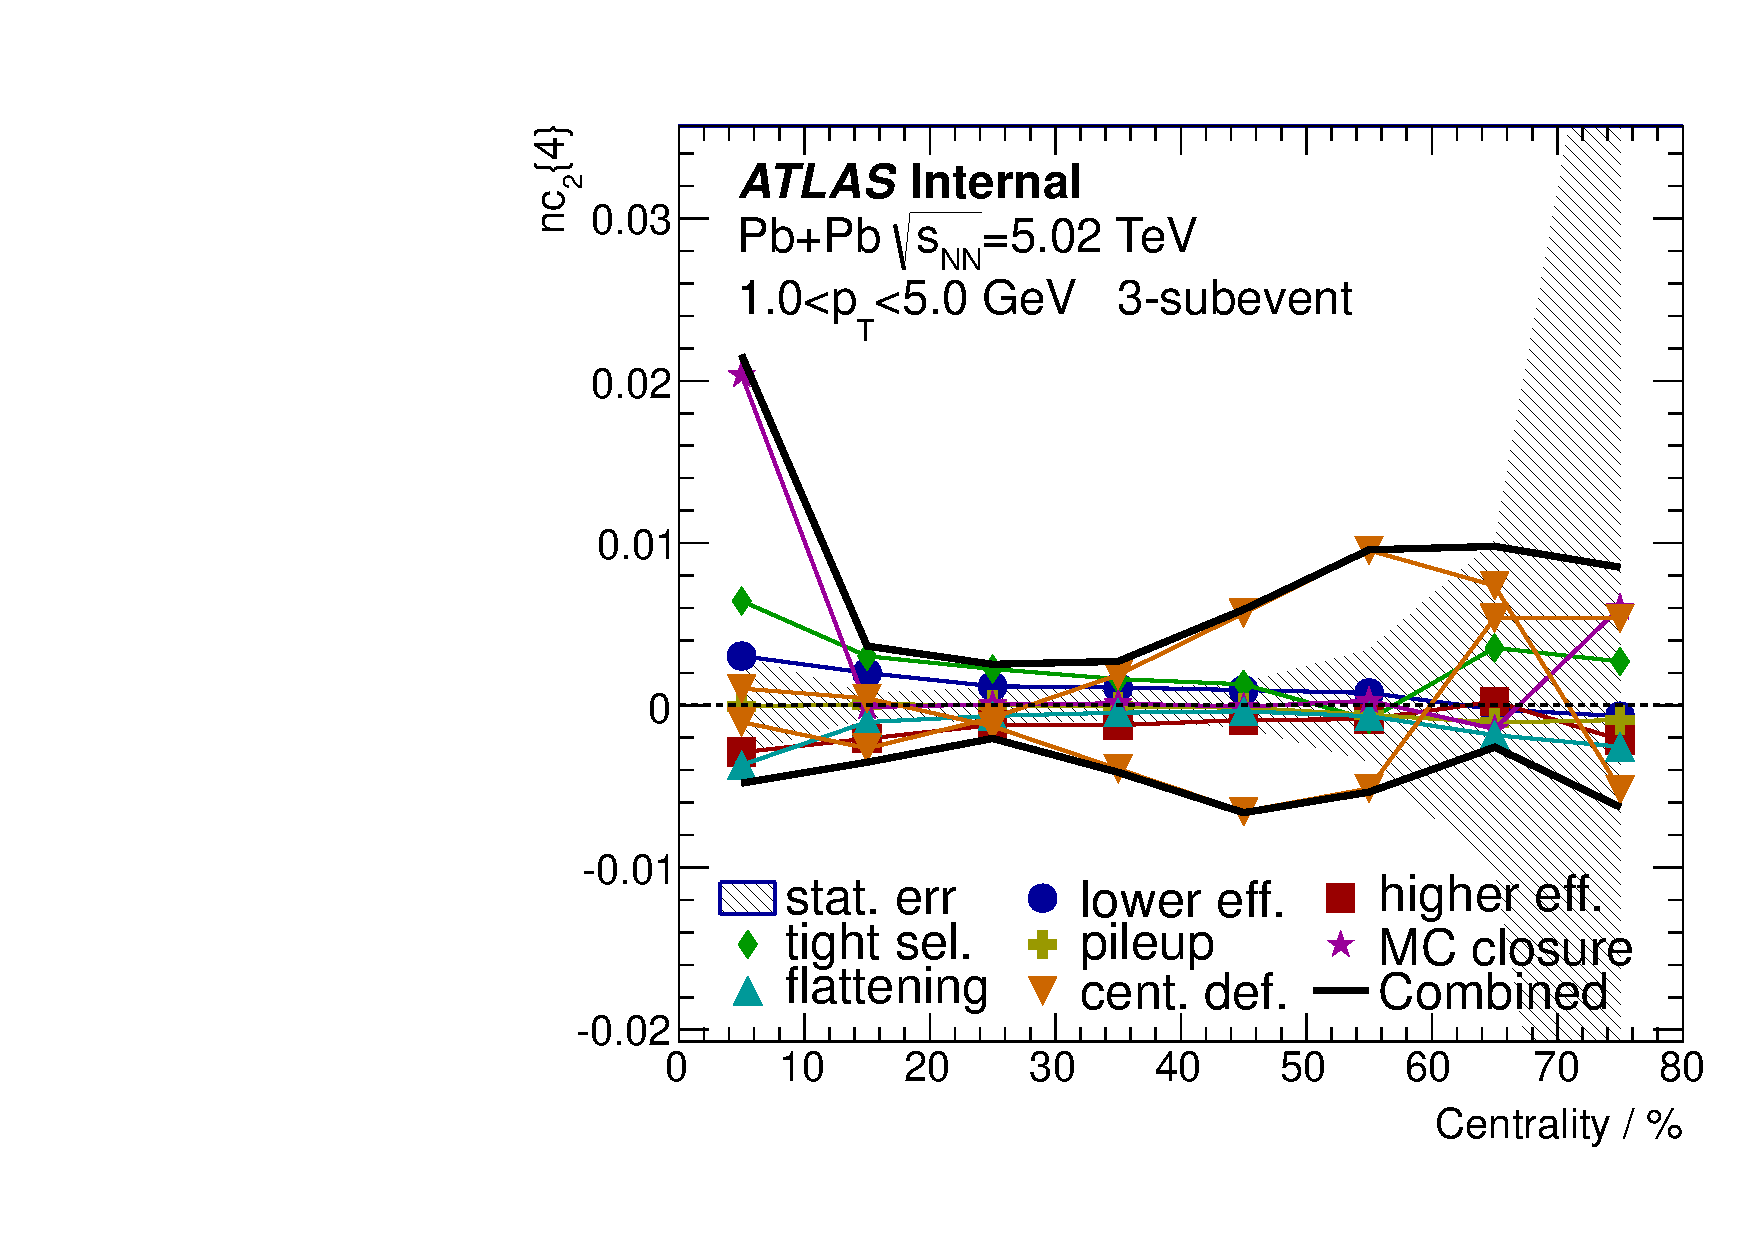
\includegraphics[width=.425\linewidth]{figs/sec_sys/summary/sys_nc4_3sub_Har2_Pt1.pdf}
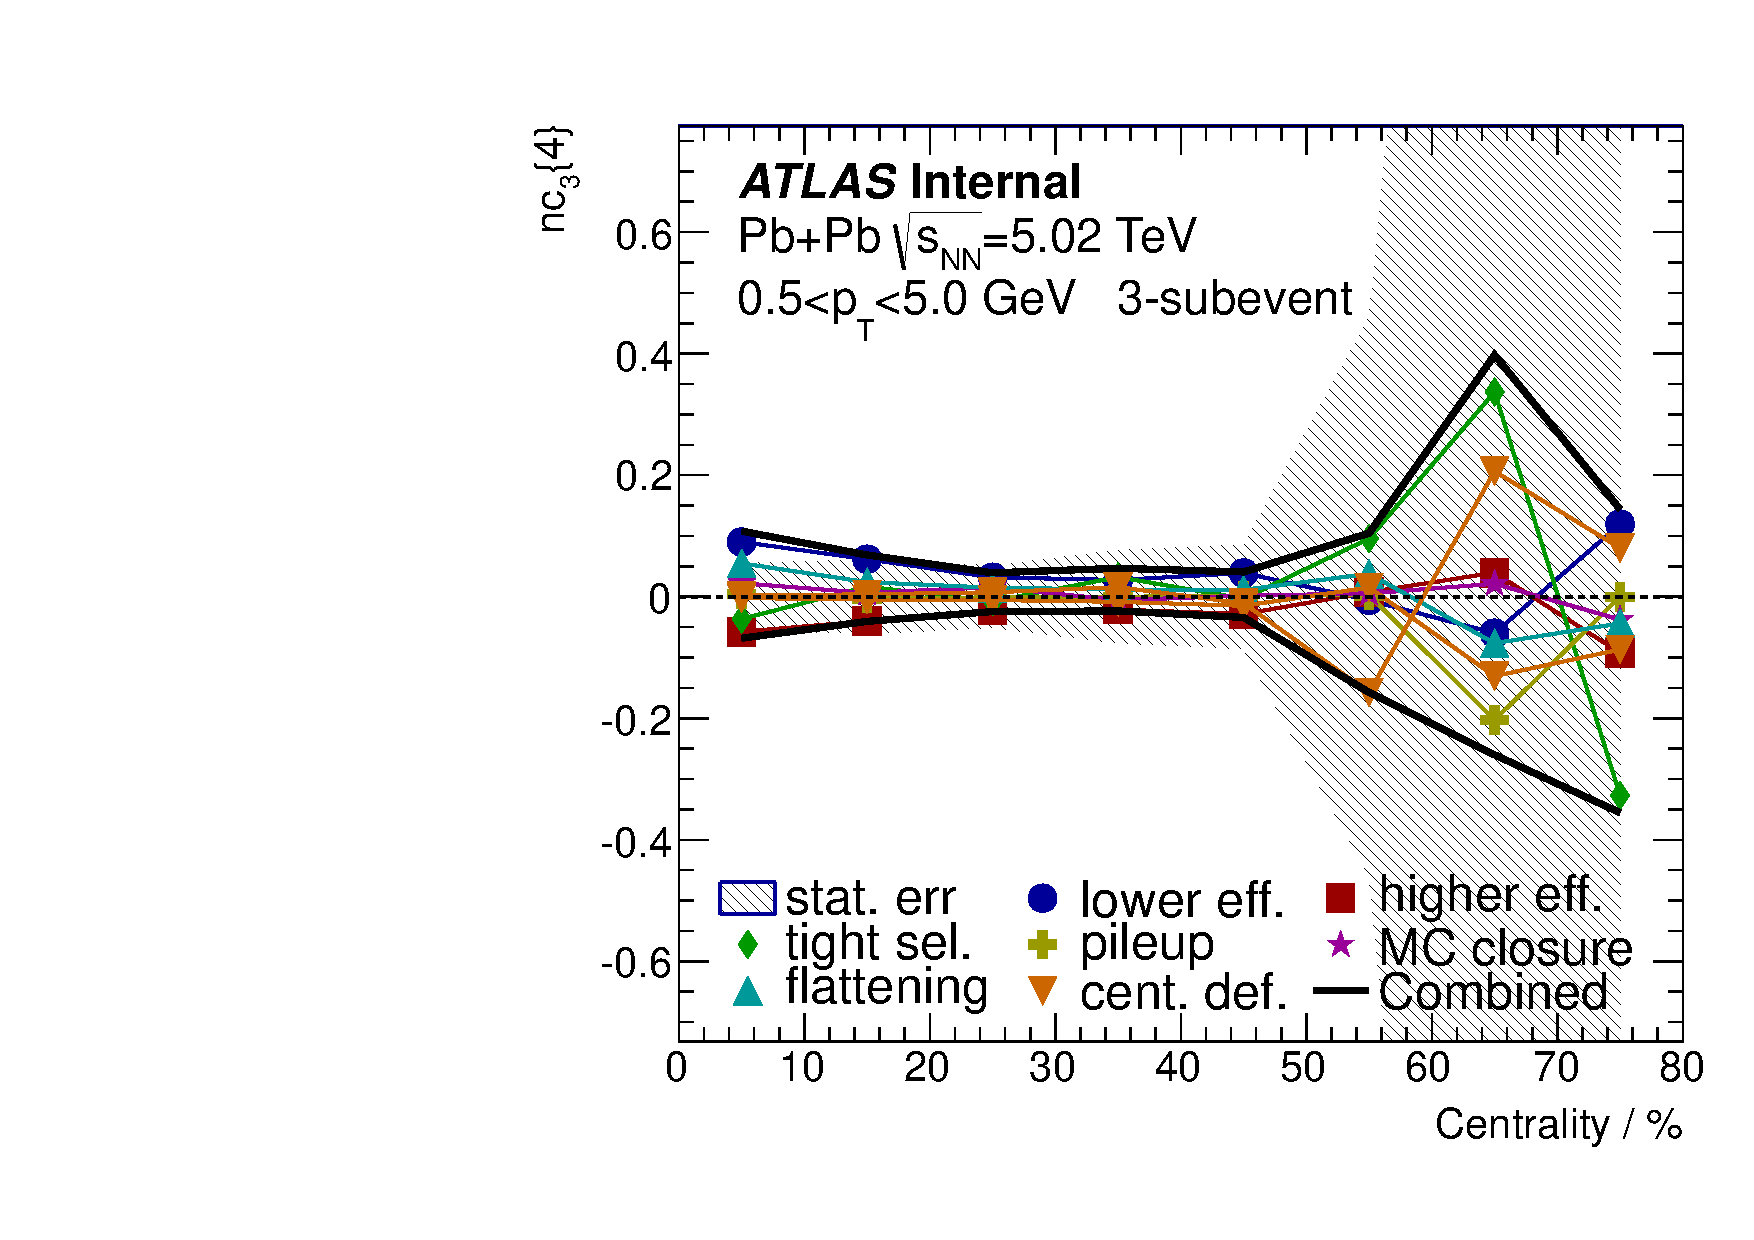
\includegraphics[width=.425\linewidth]{figs/sec_sys/summary/sys_nc4_3sub_Har3_Pt0.pdf}
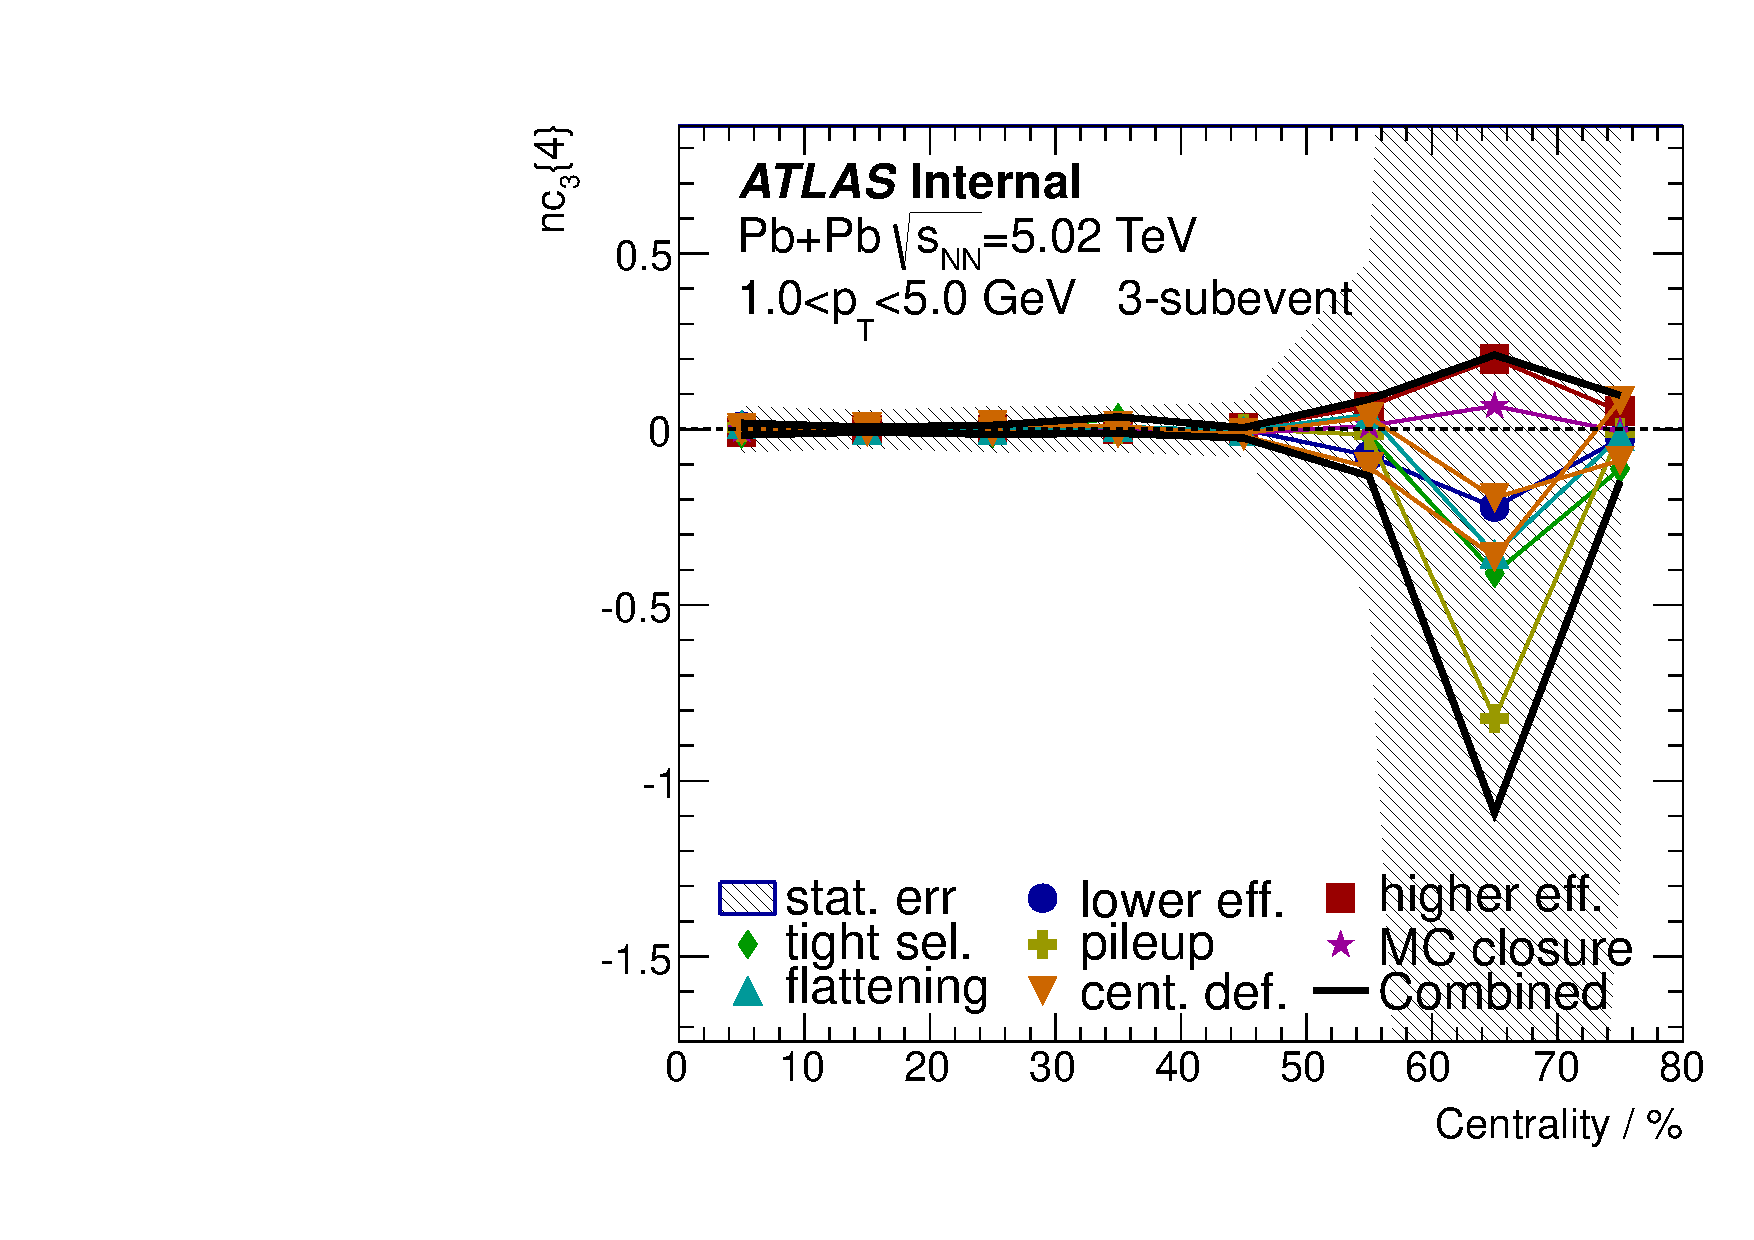
\includegraphics[width=.425\linewidth]{figs/sec_sys/summary/sys_nc4_3sub_Har3_Pt1.pdf}
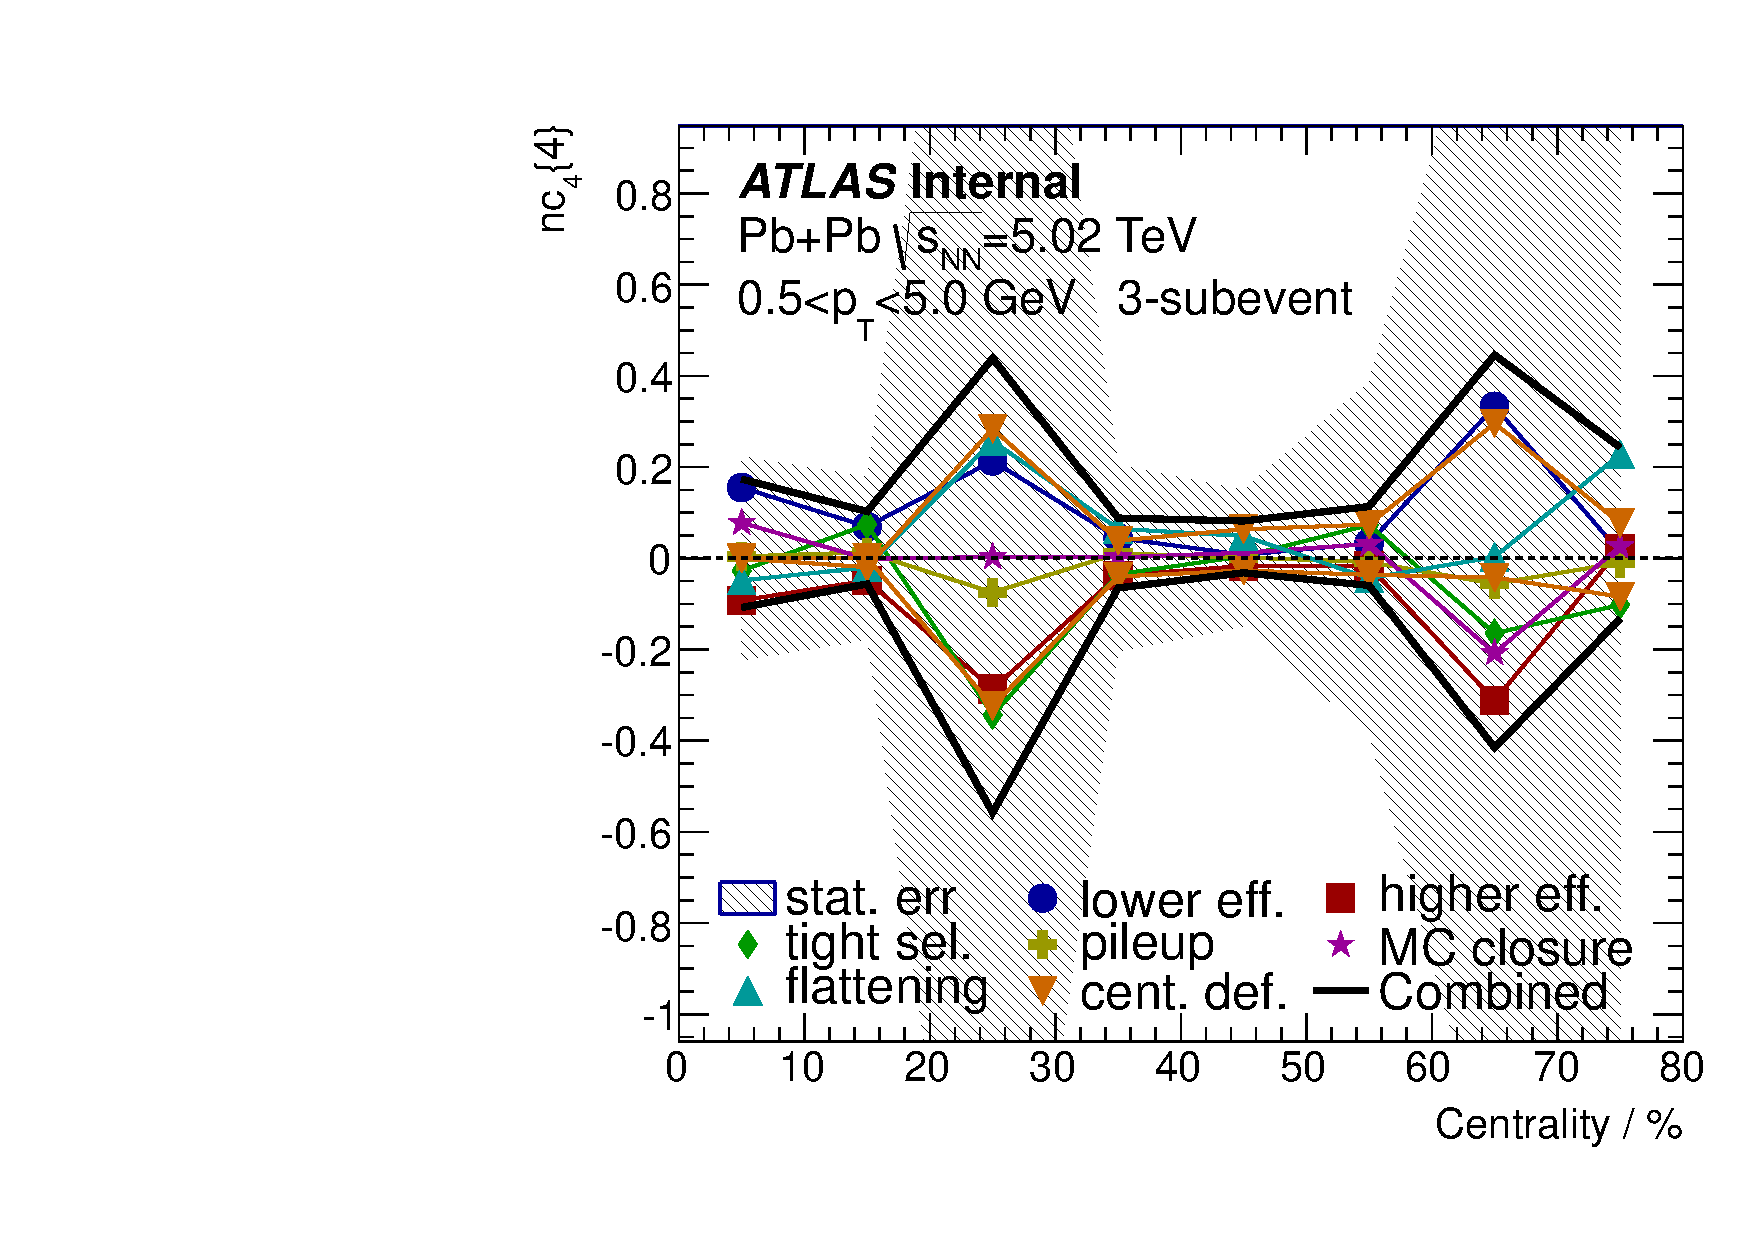
\includegraphics[width=.425\linewidth]{figs/sec_sys/summary/sys_nc4_3sub_Har4_Pt0.pdf}
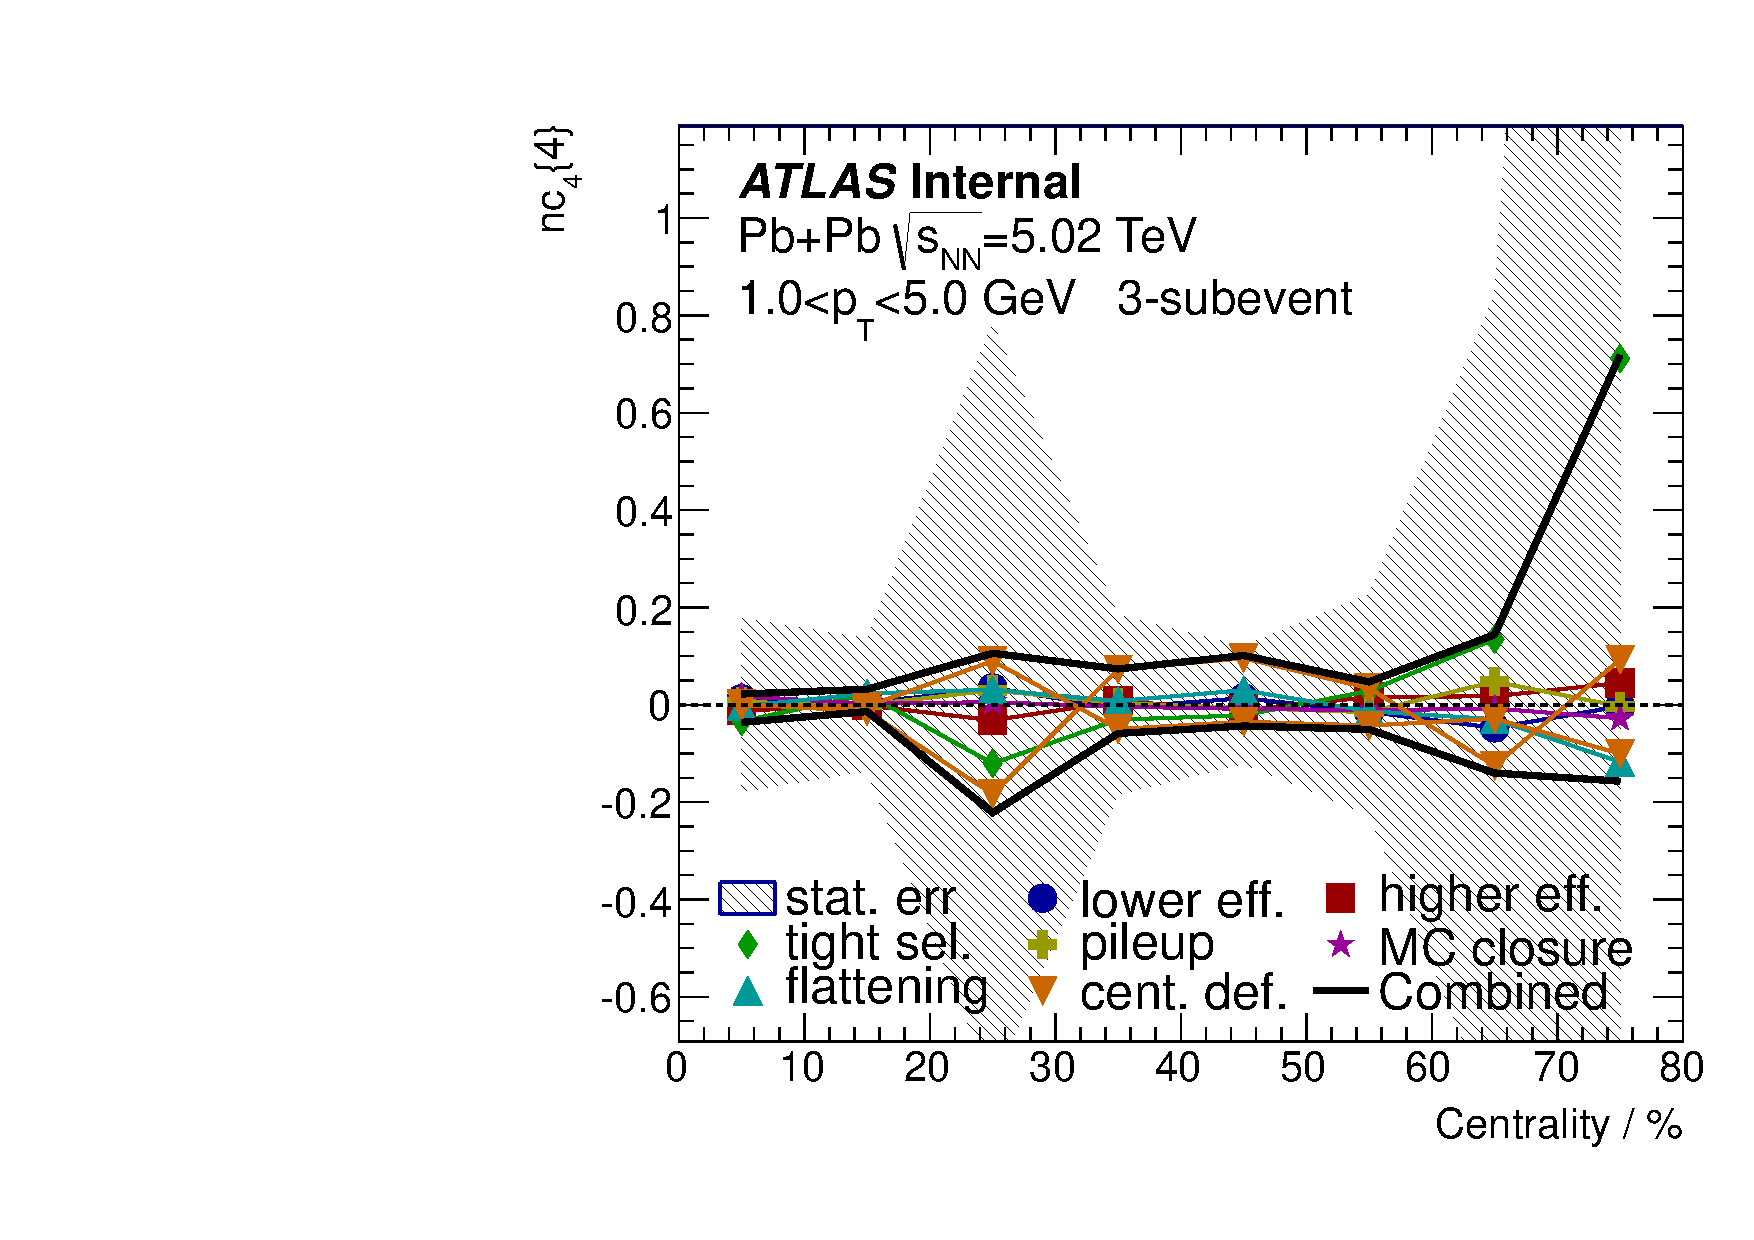
\includegraphics[width=.425\linewidth]{figs/sec_sys/summary/sys_nc4_3sub_Har4_Pt1.pdf}
\caption{Breakdown of systematics for 4-particle normalized cumulant $\hat{c}_n\{4\}$ using 3-subevent method, with low (left) and high (right) $p_\text{T}$ ranges. Different rows are for different harmonics.}
\label{fig:apdx_sys_nc4_3sub}
\end{figure}

\begin{figure}[H]
\centering
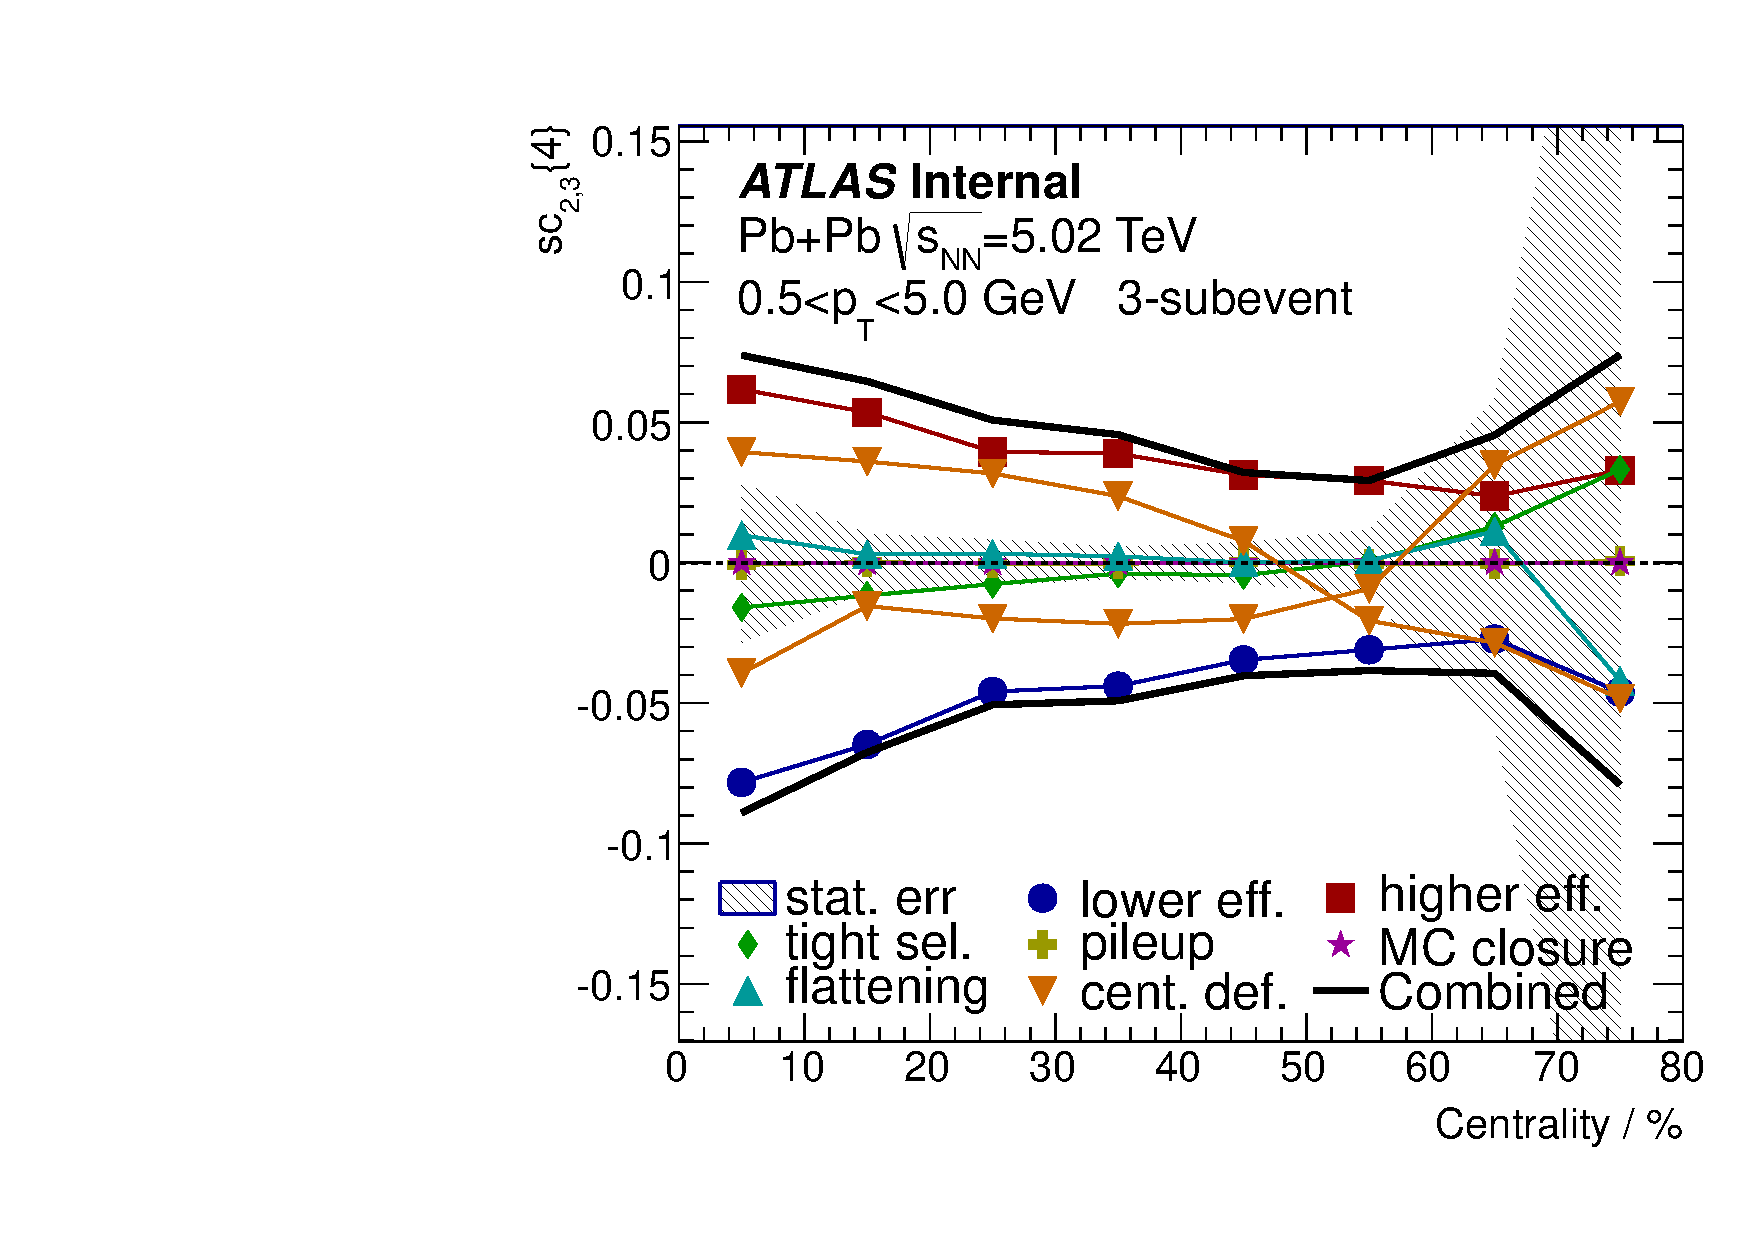
\includegraphics[width=.425\linewidth]{figs/sec_sys/summary/sys_sc_3sub_Har2_Pt0.pdf}
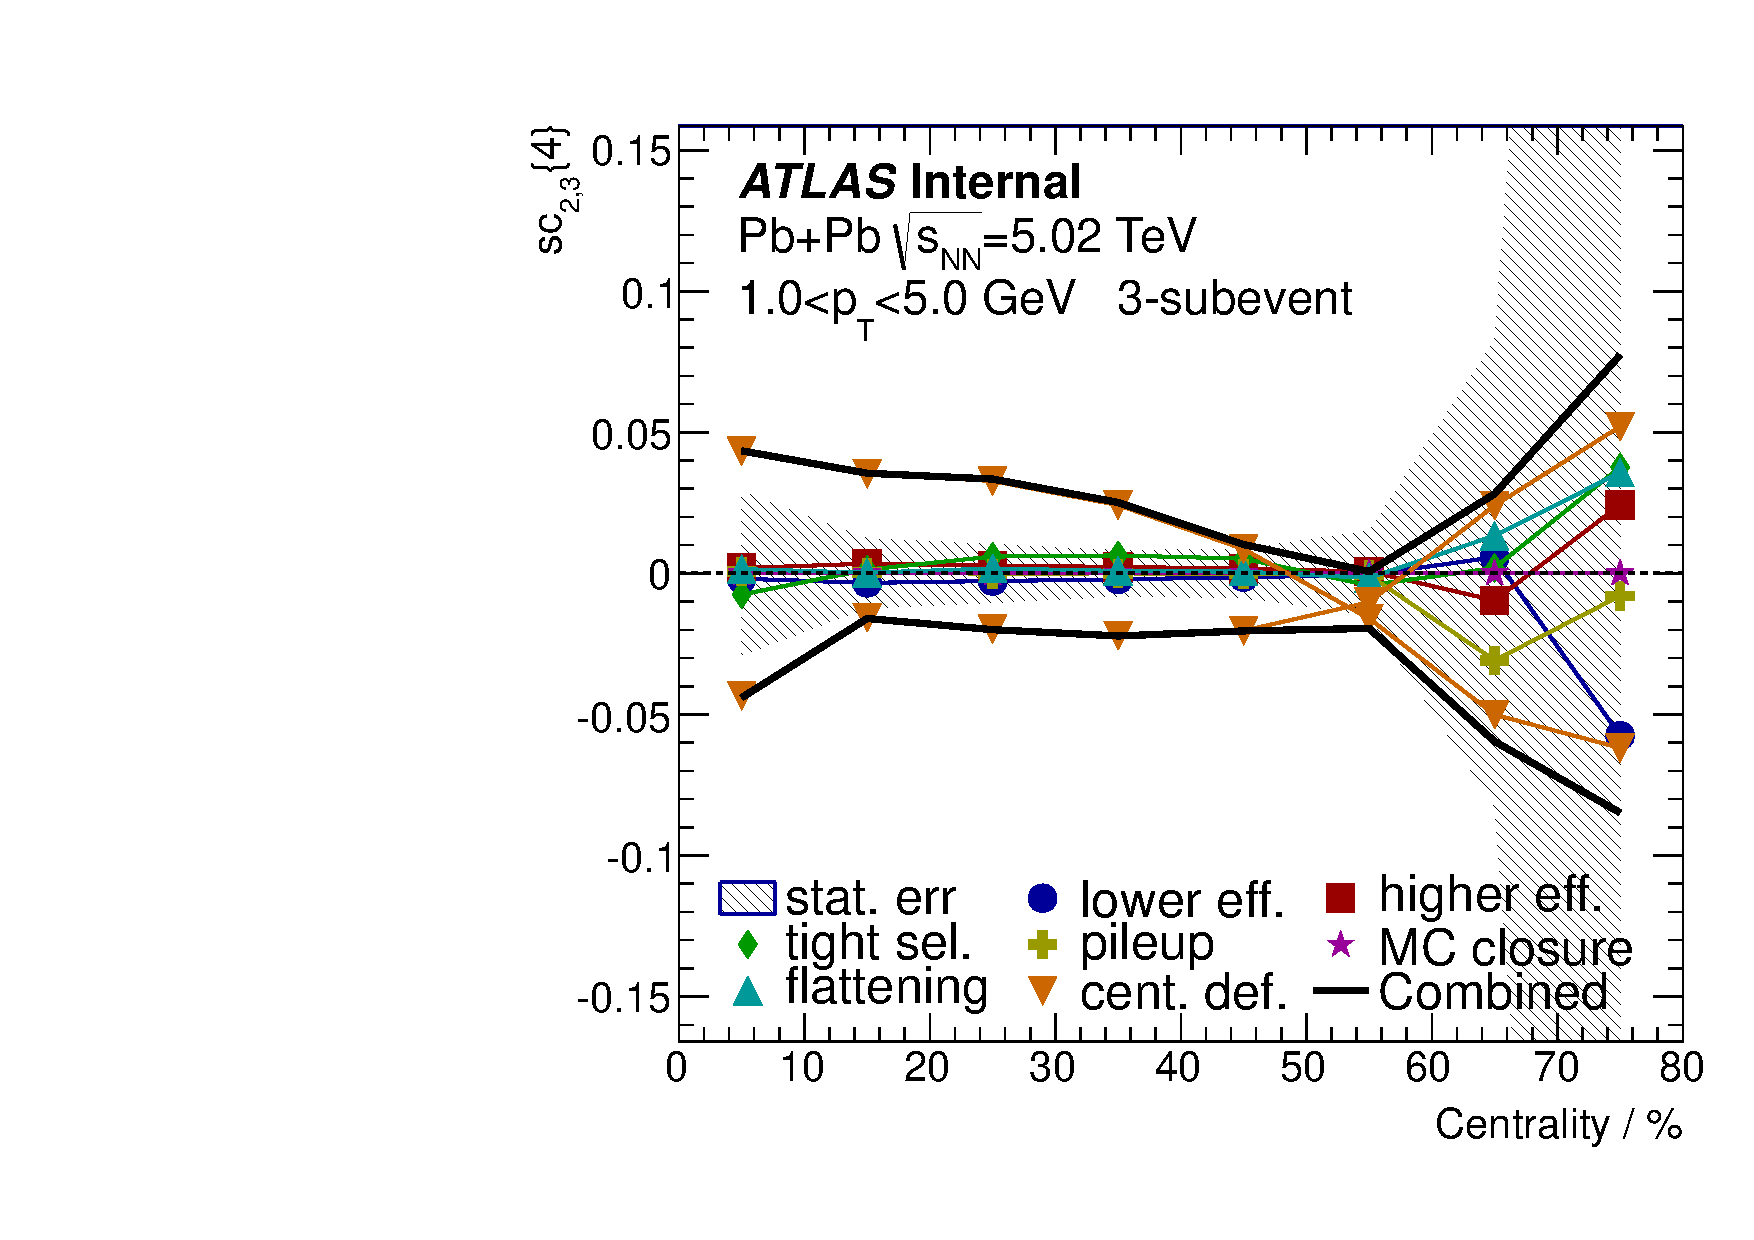
\includegraphics[width=.425\linewidth]{figs/sec_sys/summary/sys_sc_3sub_Har2_Pt1.pdf}
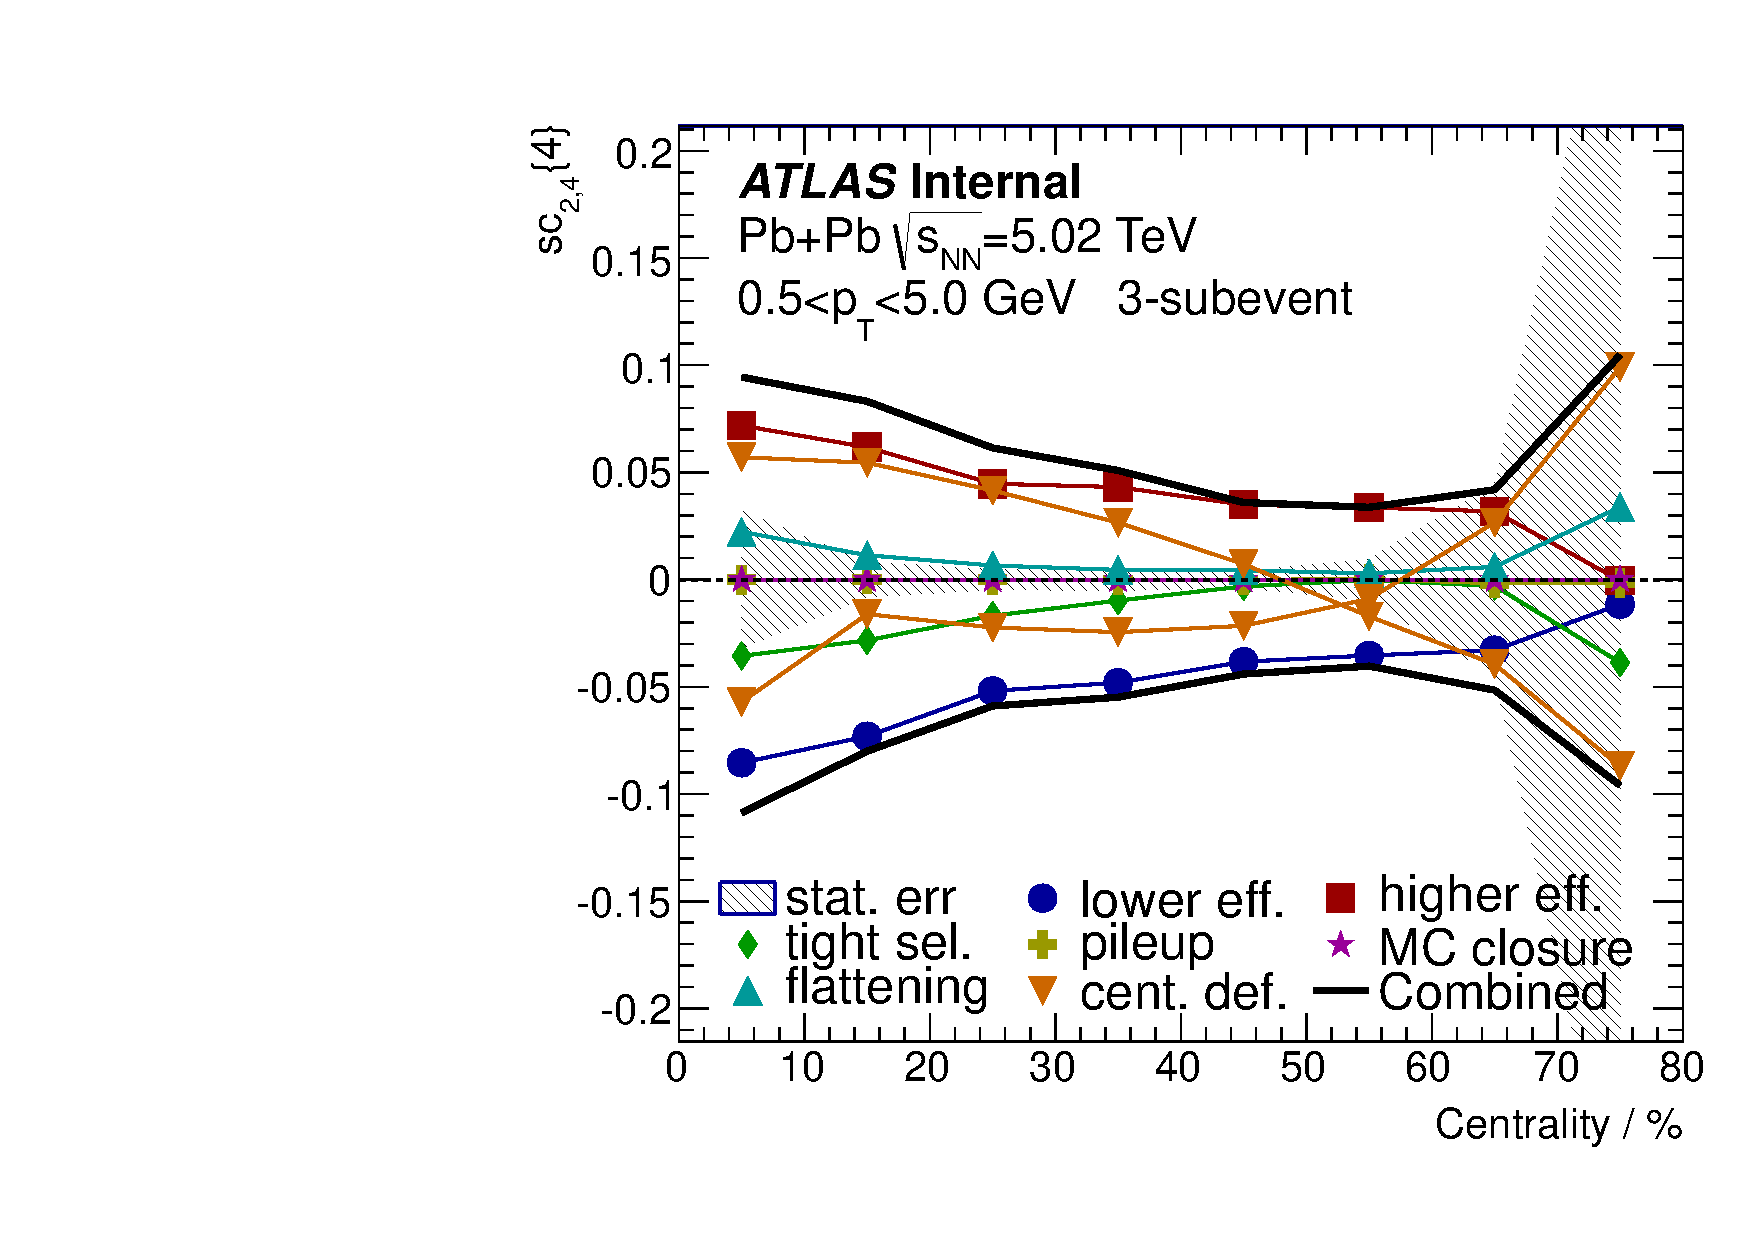
\includegraphics[width=.425\linewidth]{figs/sec_sys/summary/sys_sc_3sub_Har3_Pt0.pdf}
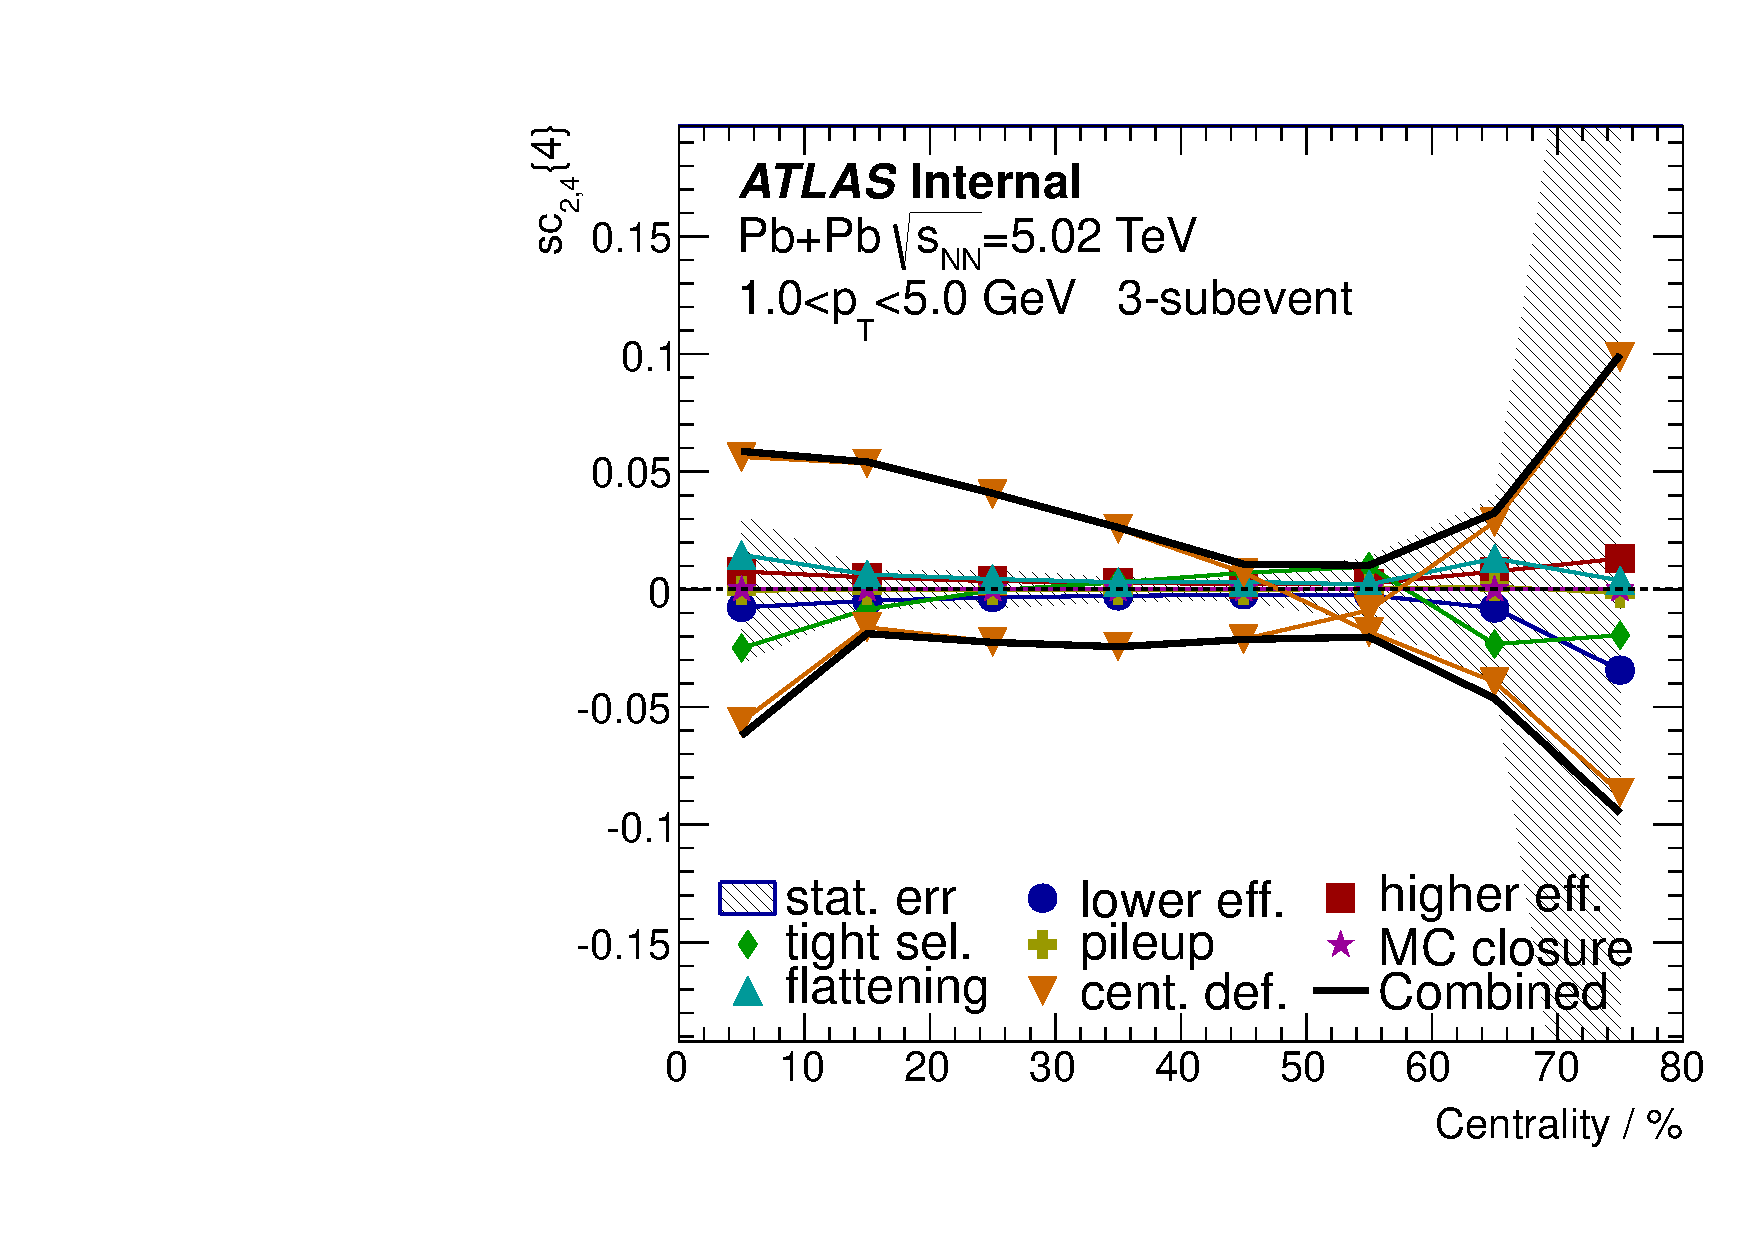
\includegraphics[width=.425\linewidth]{figs/sec_sys/summary/sys_sc_3sub_Har3_Pt1.pdf}
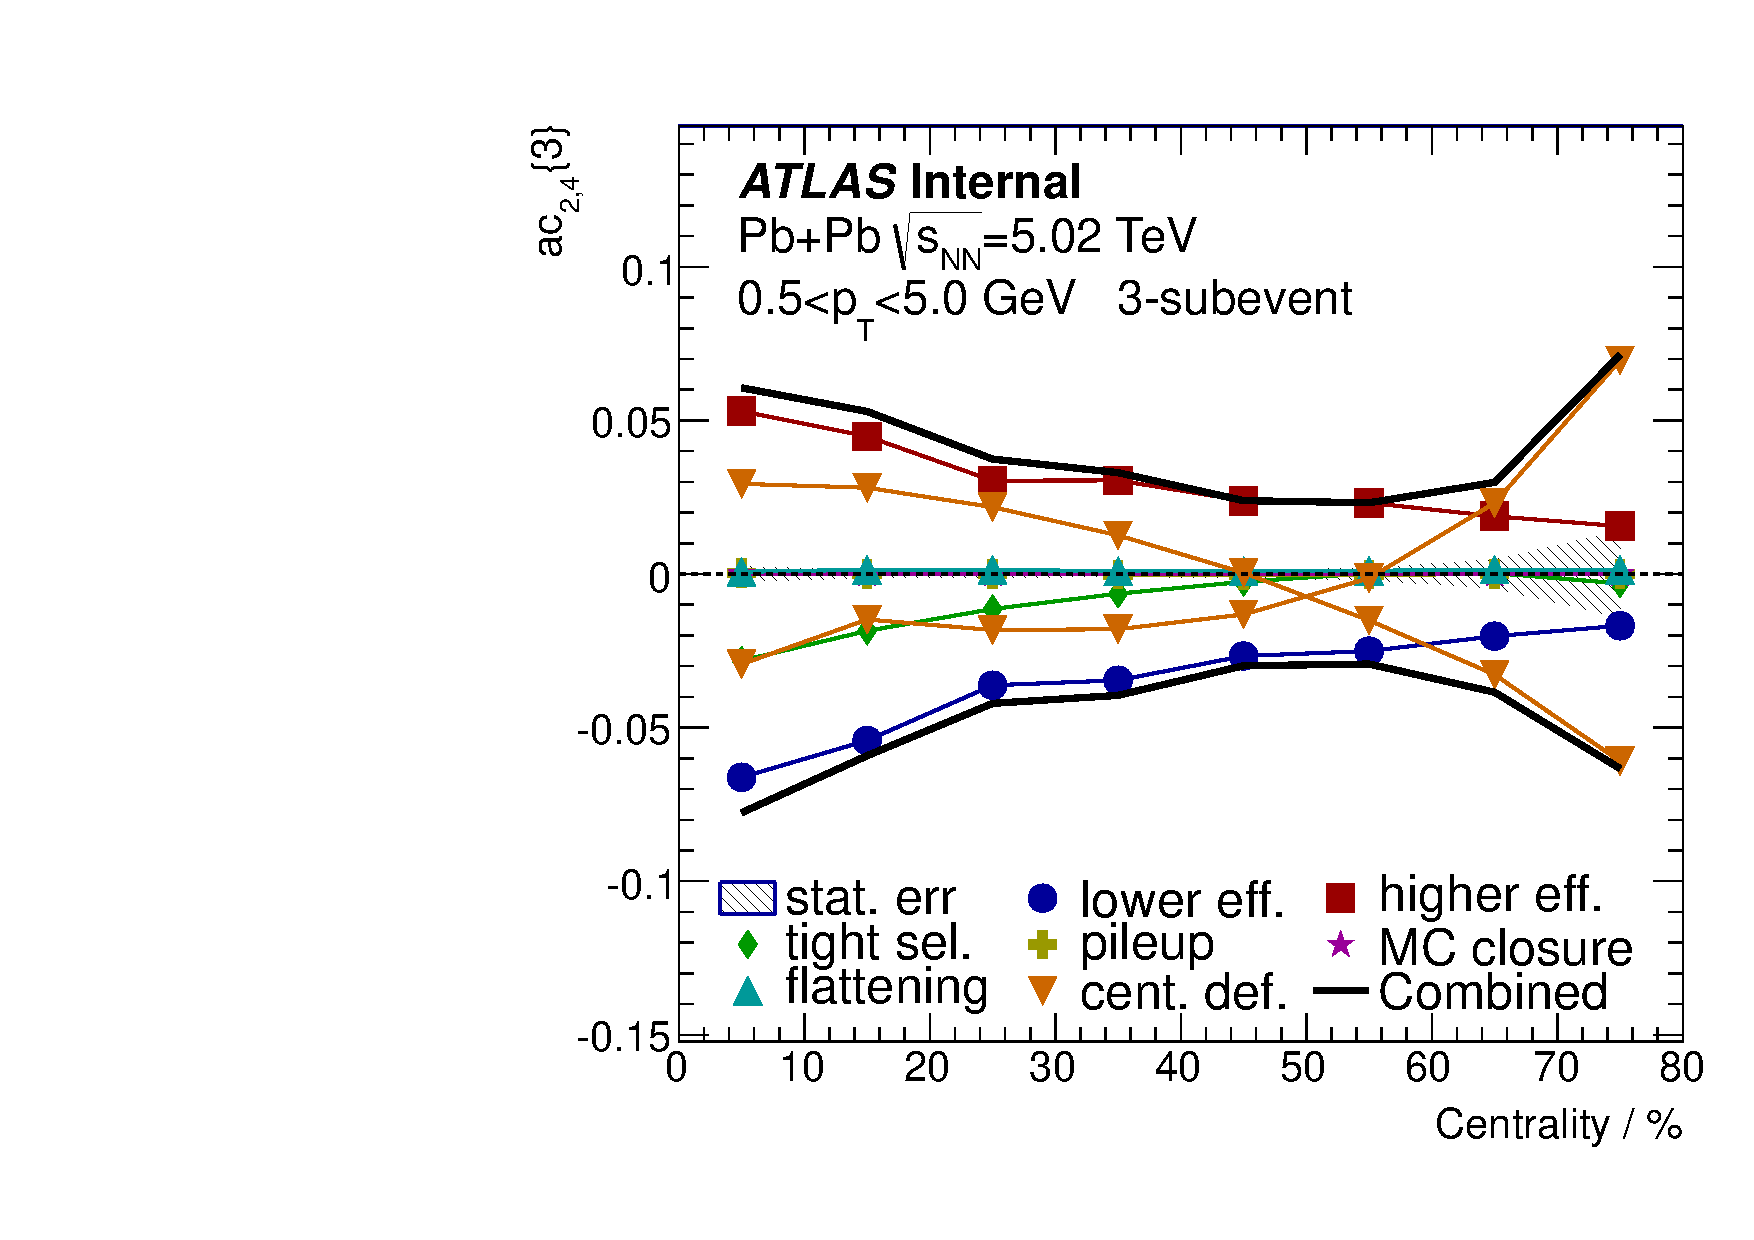
\includegraphics[width=.425\linewidth]{figs/sec_sys/summary/sys_ac_3sub_Har2_Pt0.pdf}
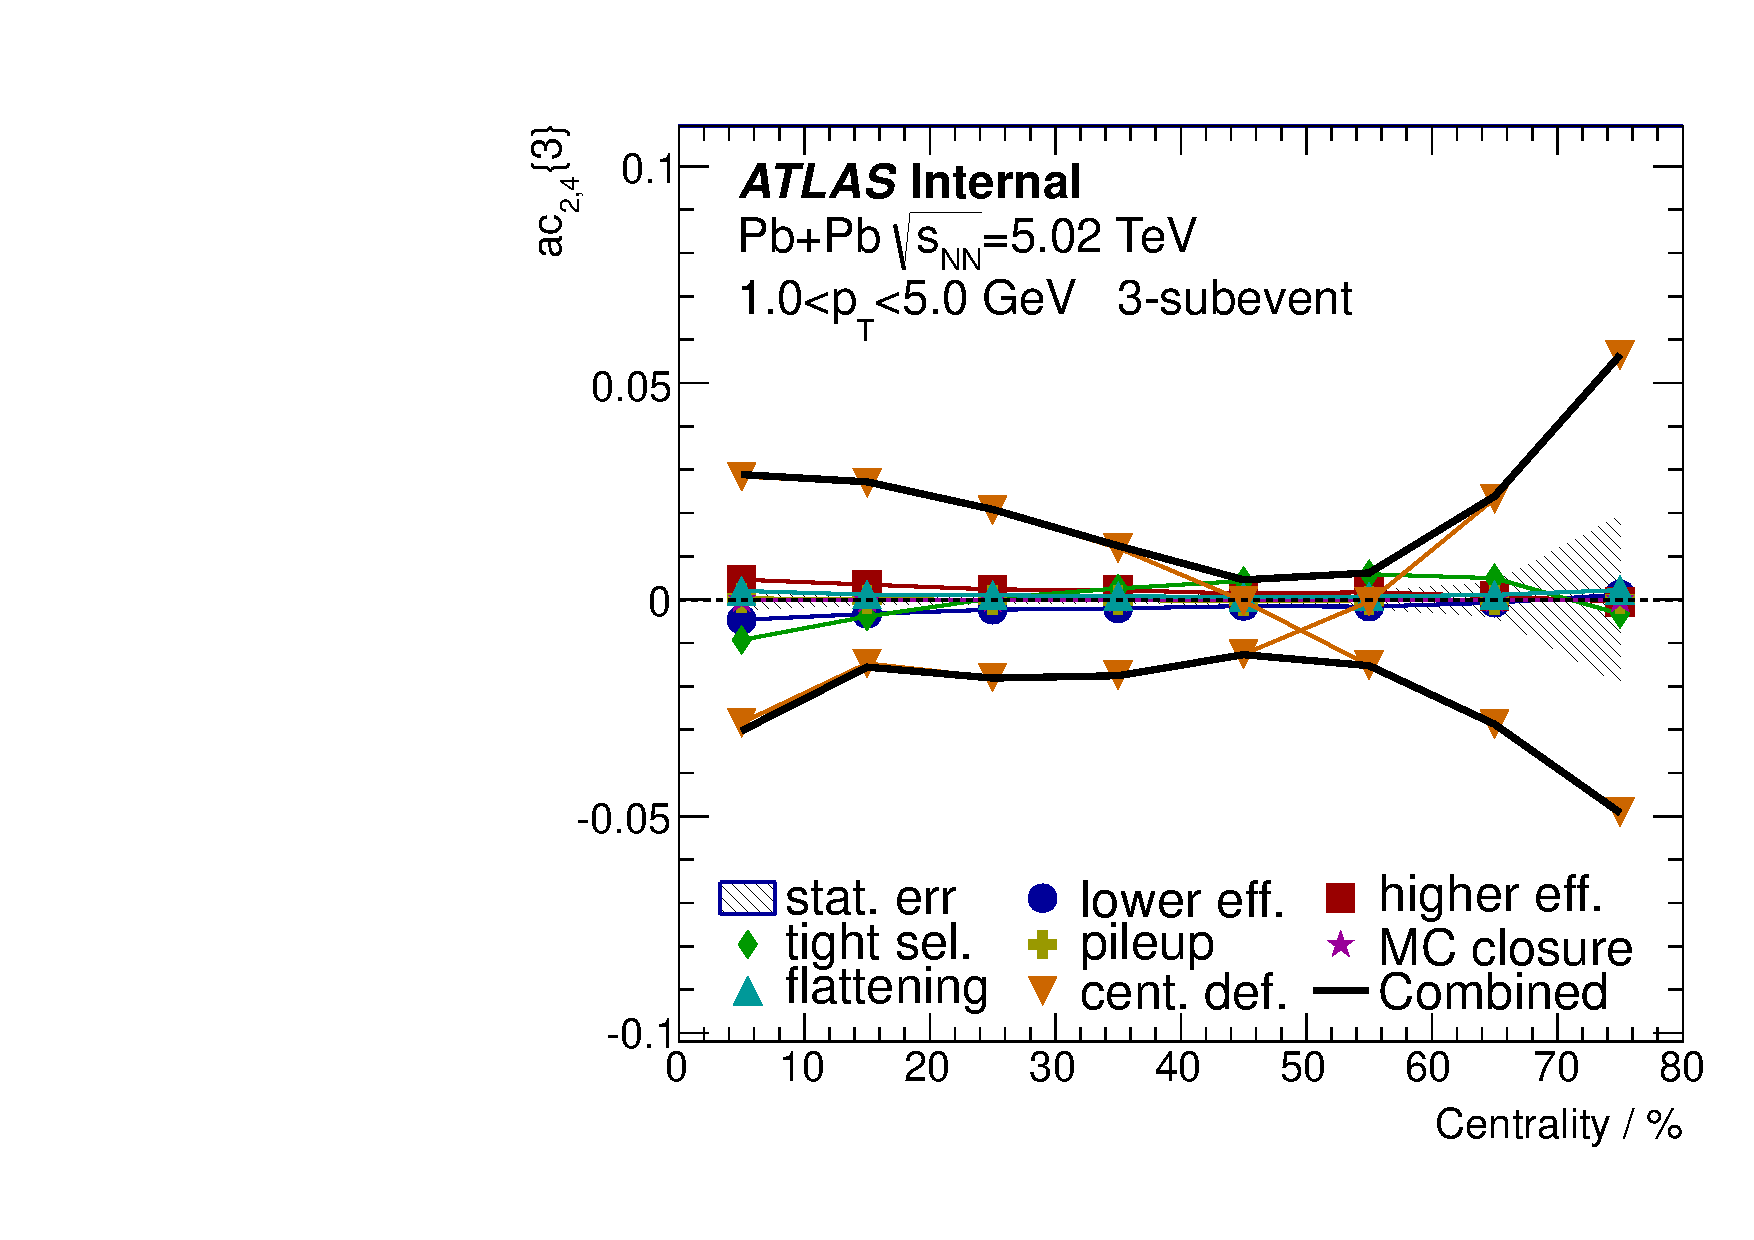
\includegraphics[width=.425\linewidth]{figs/sec_sys/summary/sys_ac_3sub_Har2_Pt1.pdf}
\caption{Breakdown of systematics for symmetric and asymmetric cumulants, using 3-subevent method, with low (left) and high (right) $p_\text{T}$ ranges. Different rows are for different harmonics.}
\label{fig:apdx_sys_sc_3sub}
\end{figure}

\begin{figure}[H]
\centering
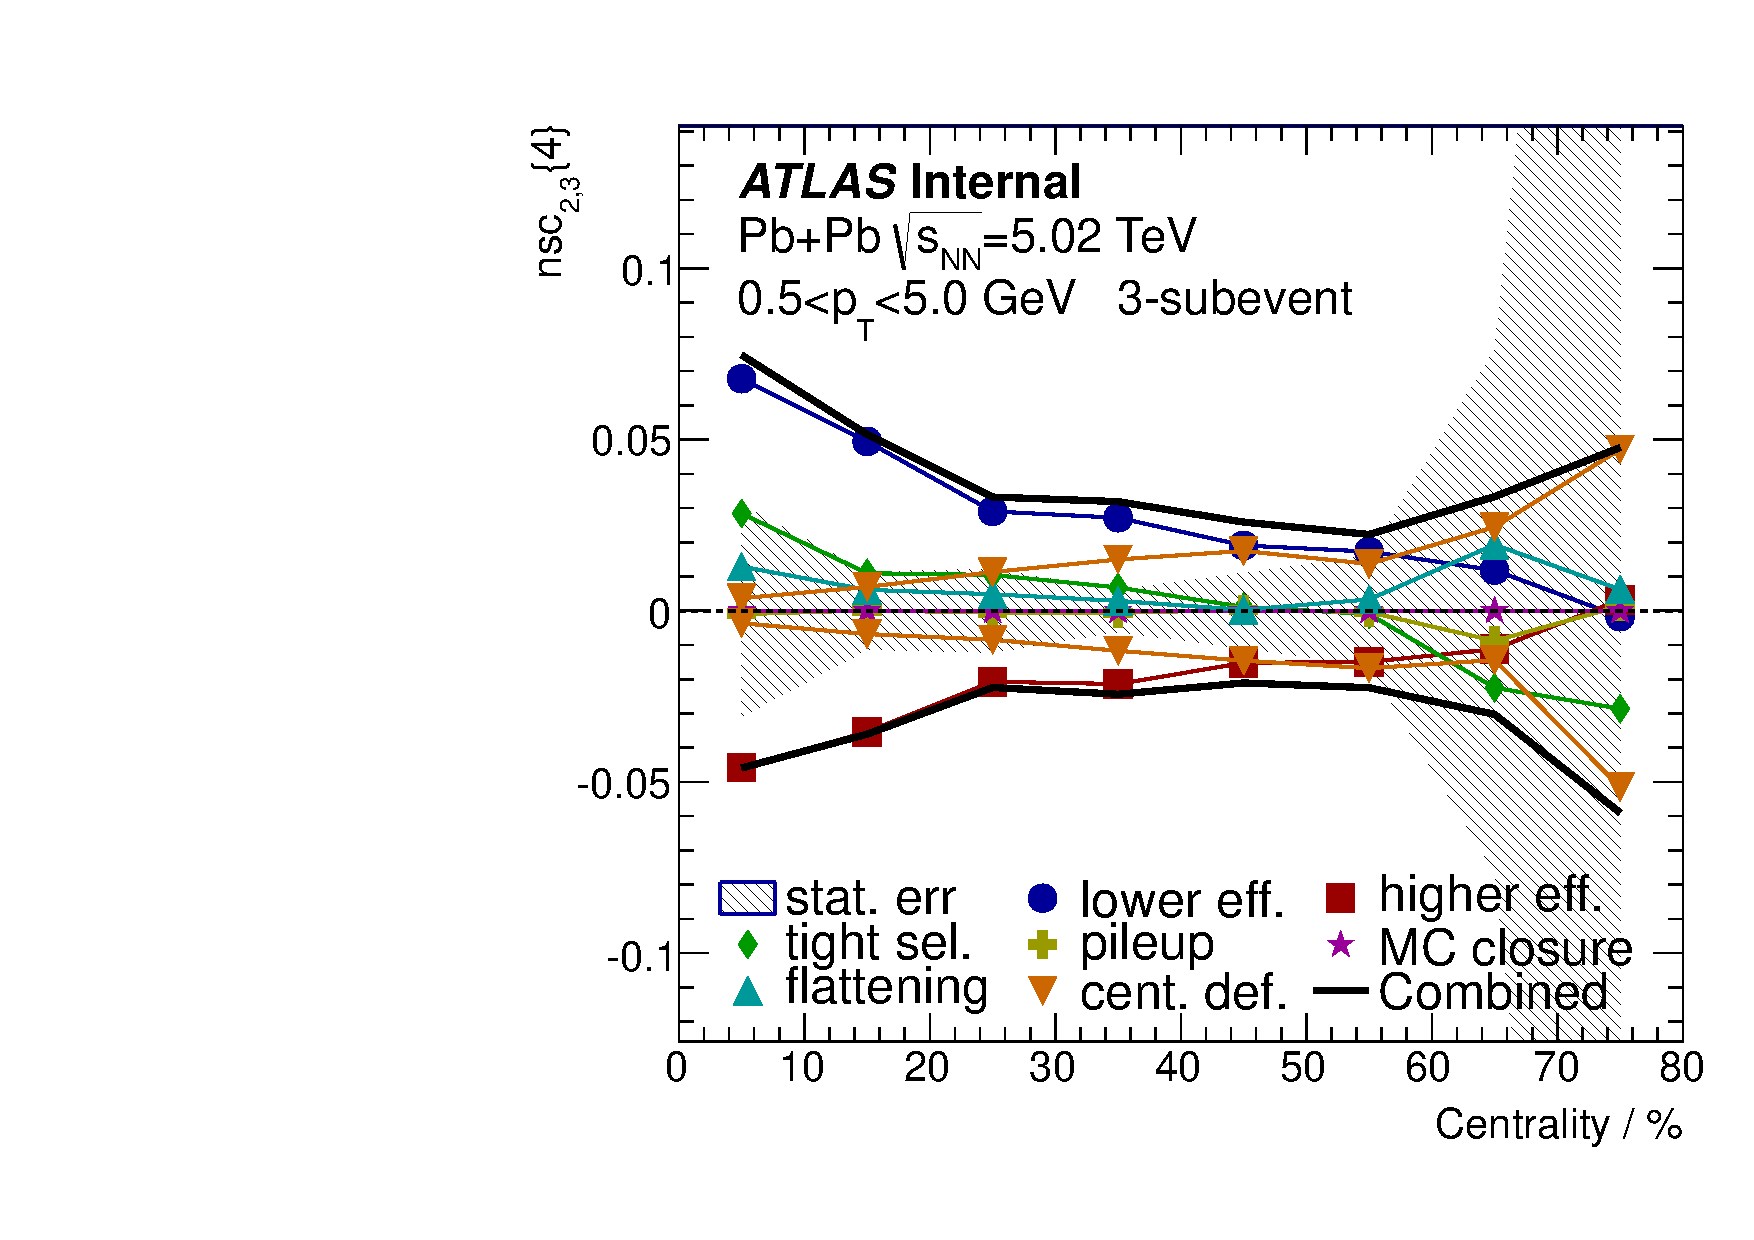
\includegraphics[width=.425\linewidth]{figs/sec_sys/summary/sys_nsc_3sub_Har2_Pt0.pdf}
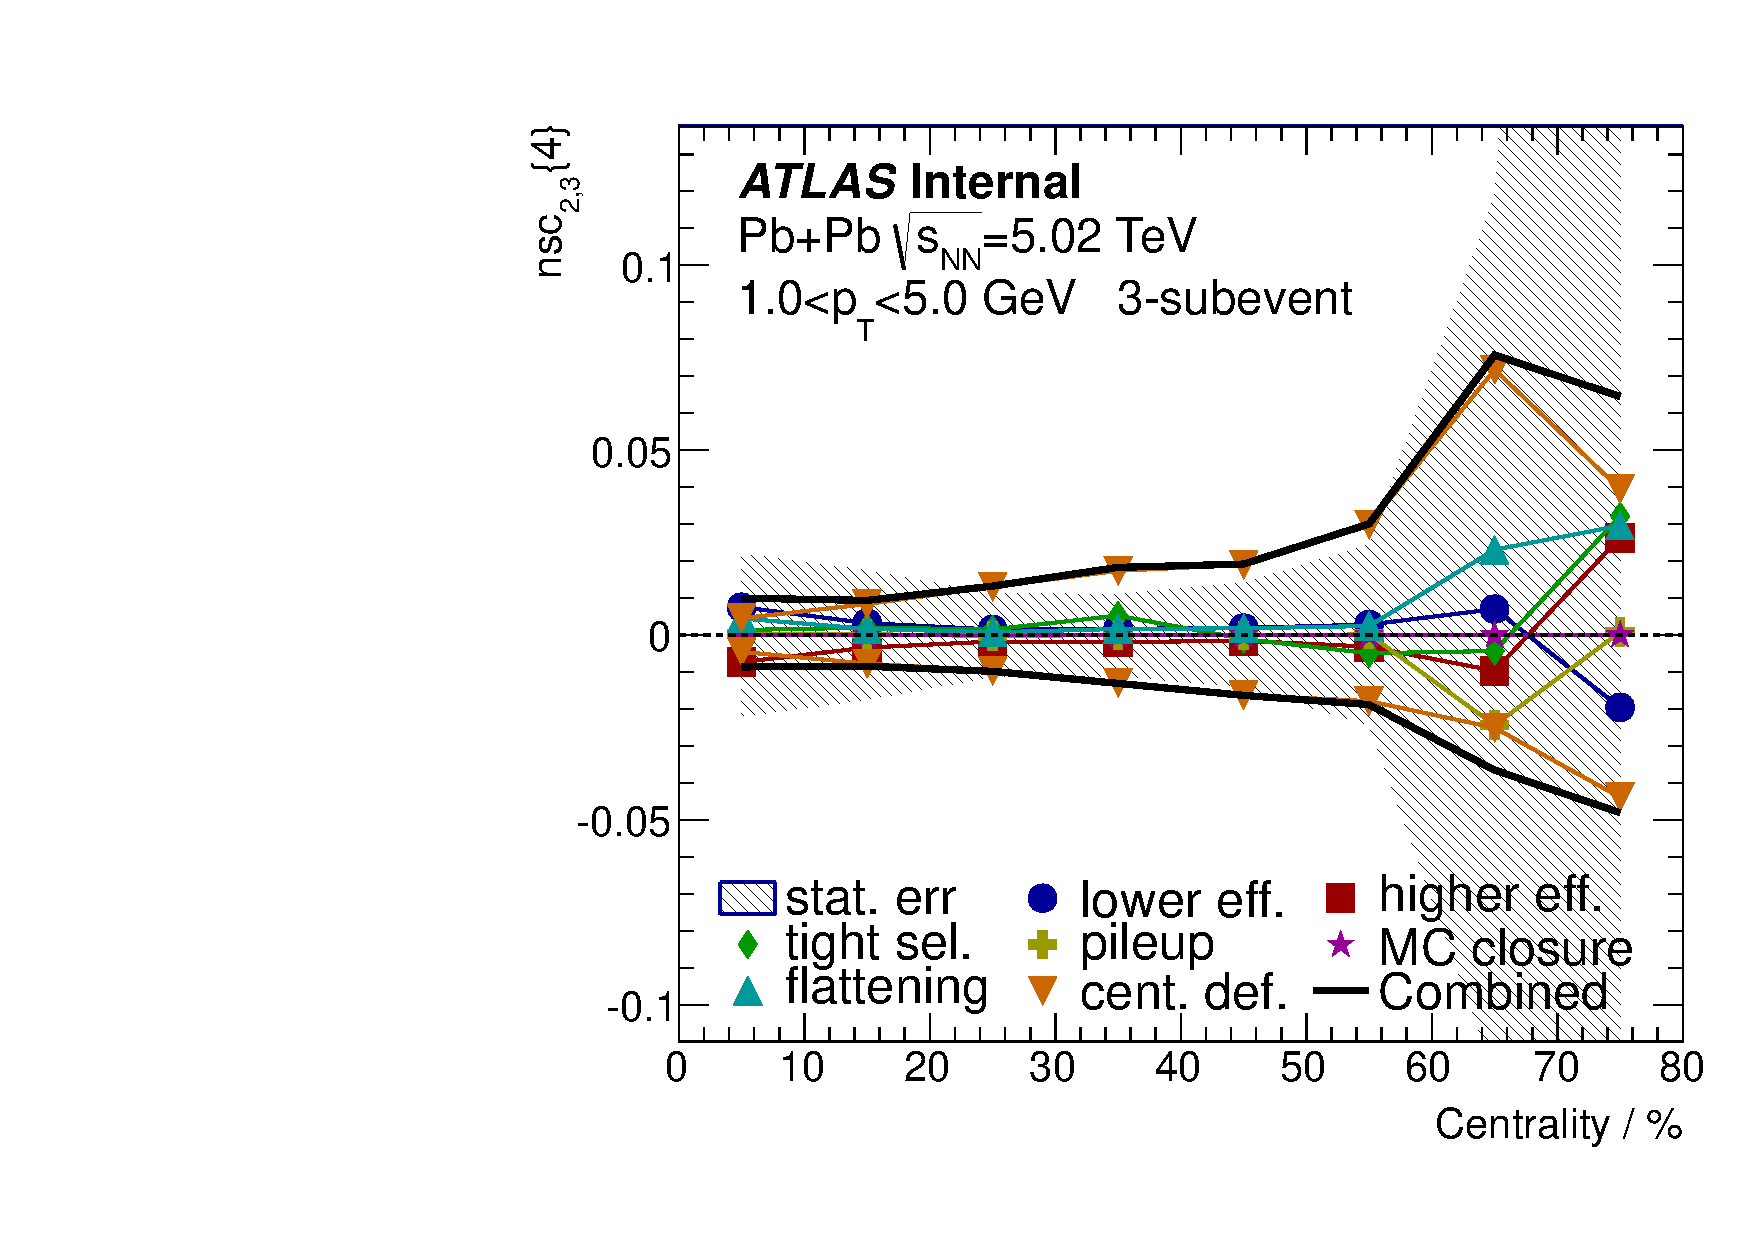
\includegraphics[width=.425\linewidth]{figs/sec_sys/summary/sys_nsc_3sub_Har2_Pt1.pdf}
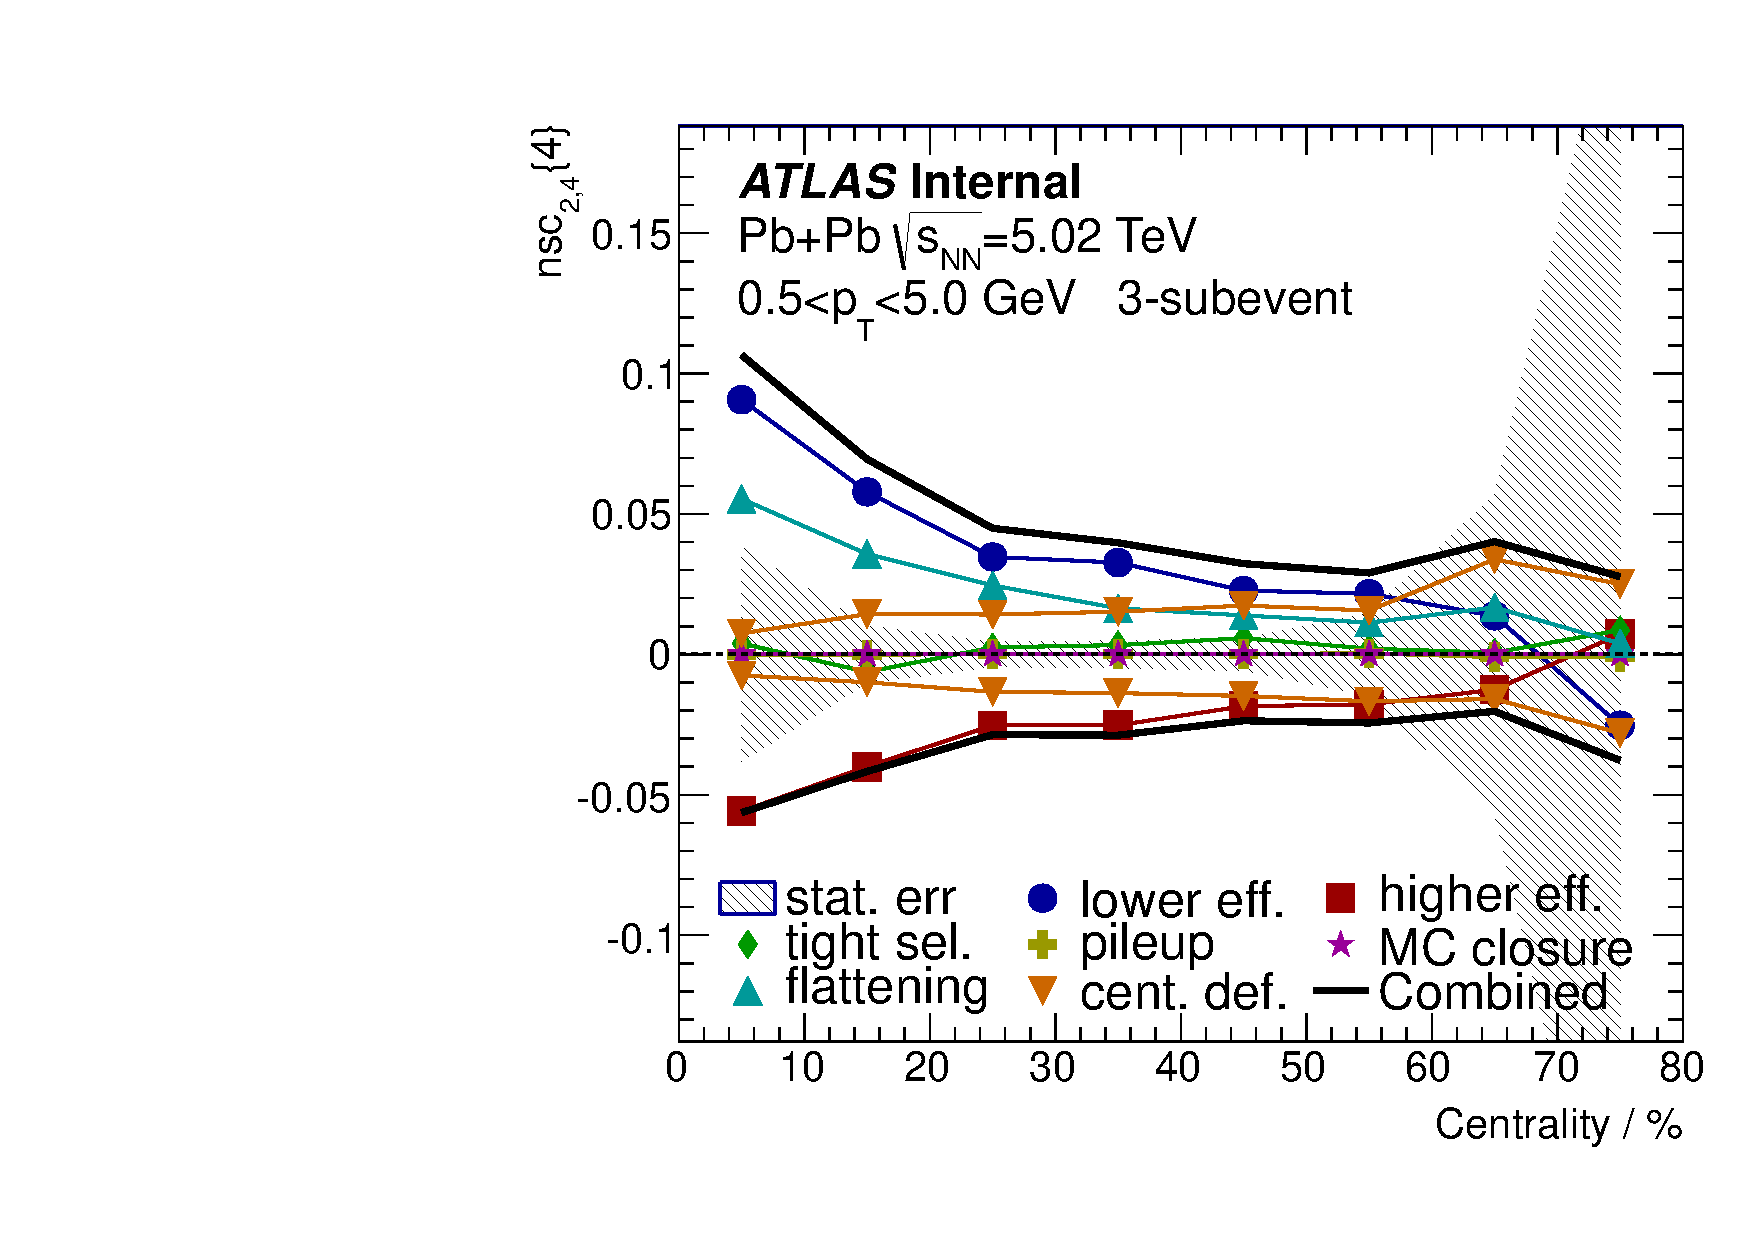
\includegraphics[width=.425\linewidth]{figs/sec_sys/summary/sys_nsc_3sub_Har3_Pt0.pdf}
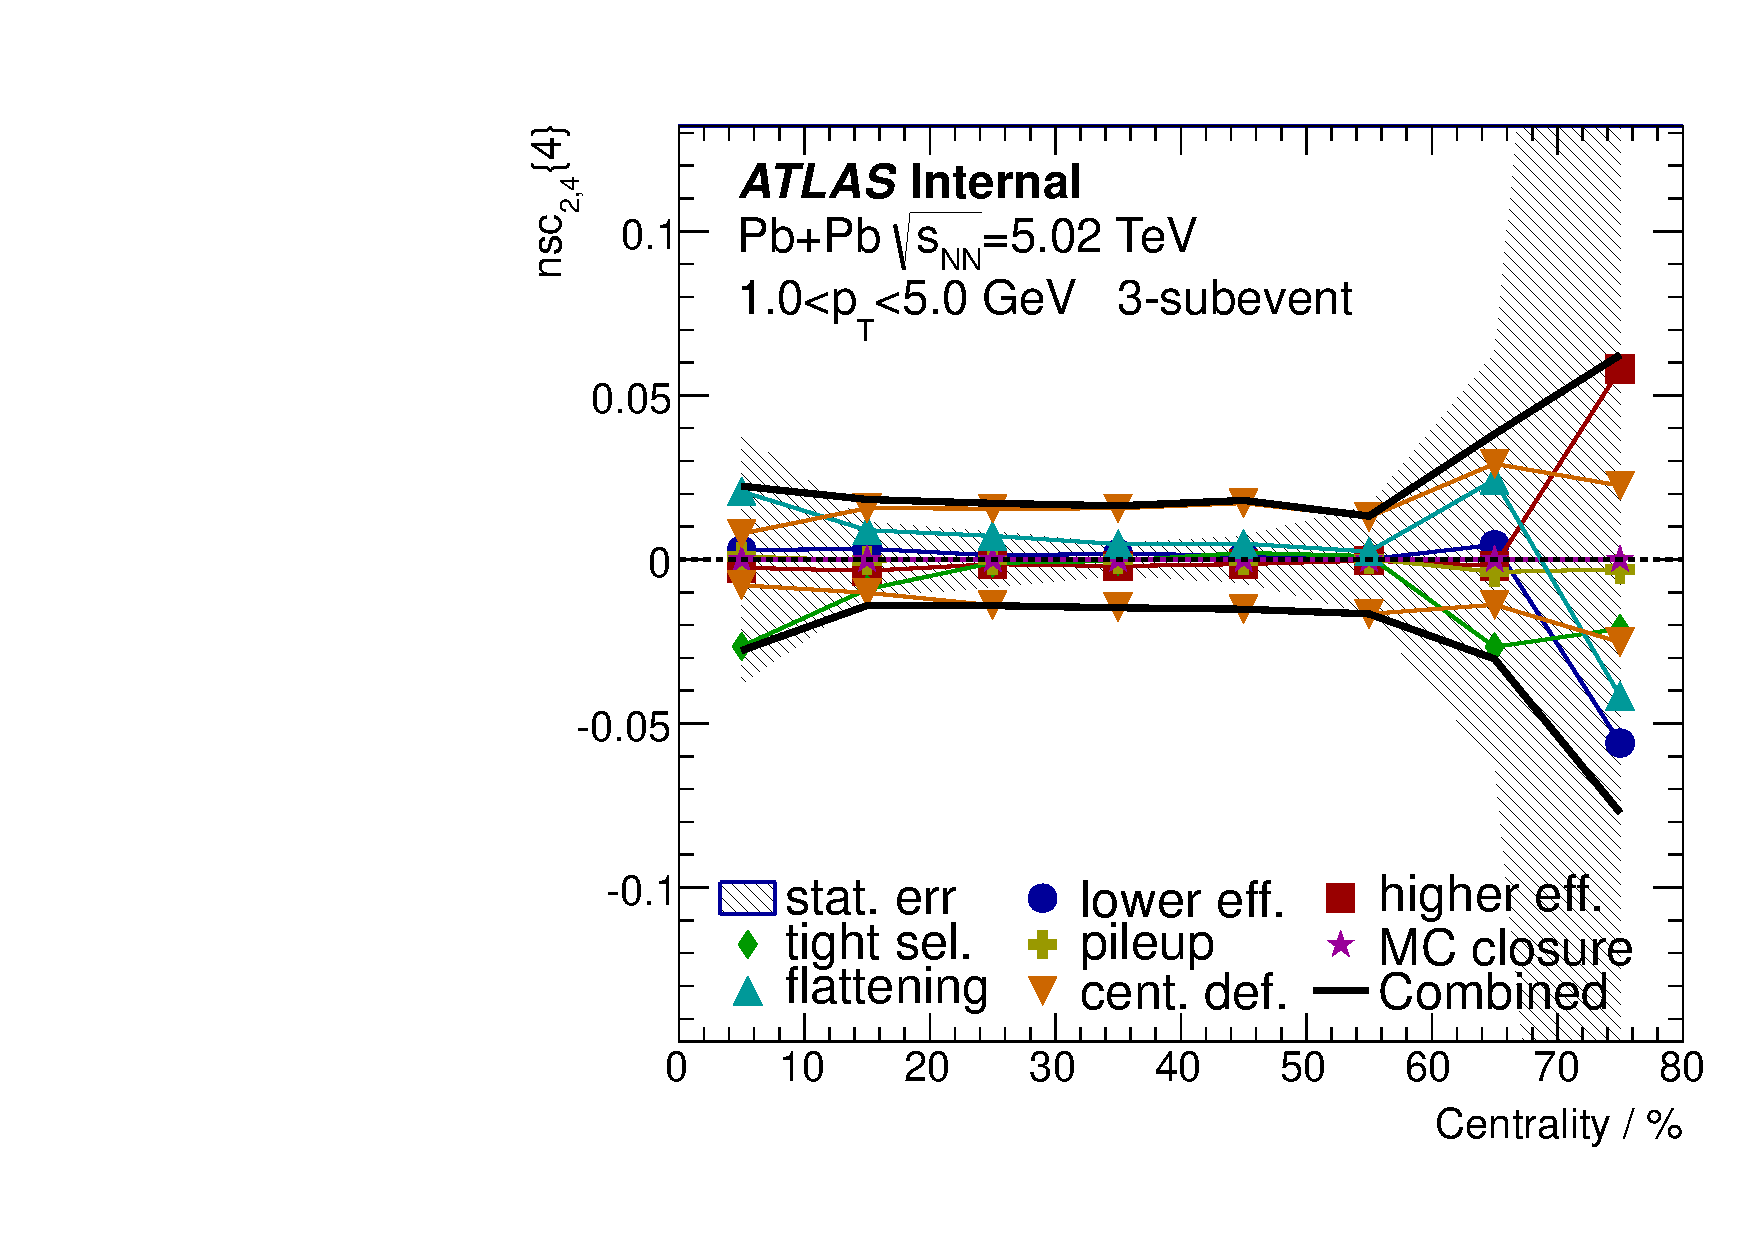
\includegraphics[width=.425\linewidth]{figs/sec_sys/summary/sys_nsc_3sub_Har3_Pt1.pdf}
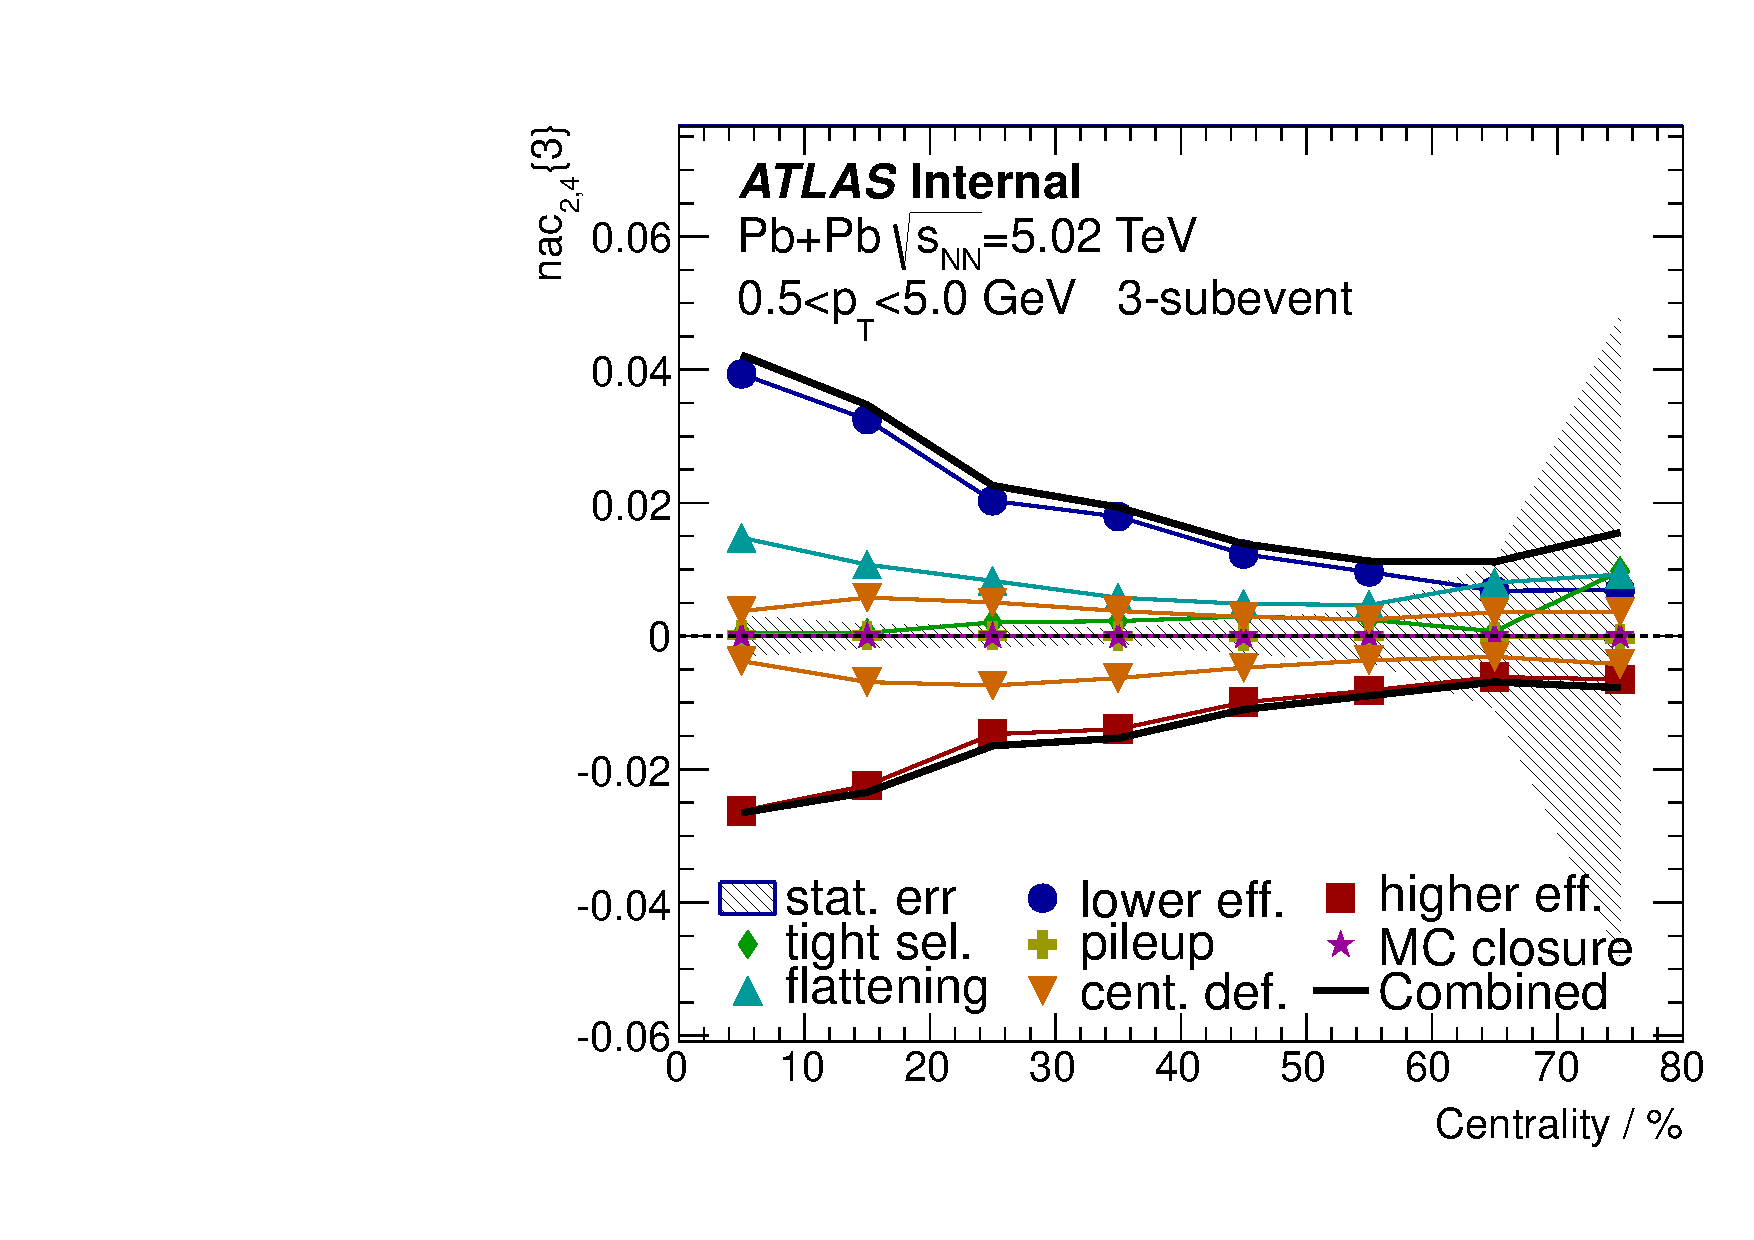
\includegraphics[width=.425\linewidth]{figs/sec_sys/summary/sys_nac_3sub_Har2_Pt0.pdf}
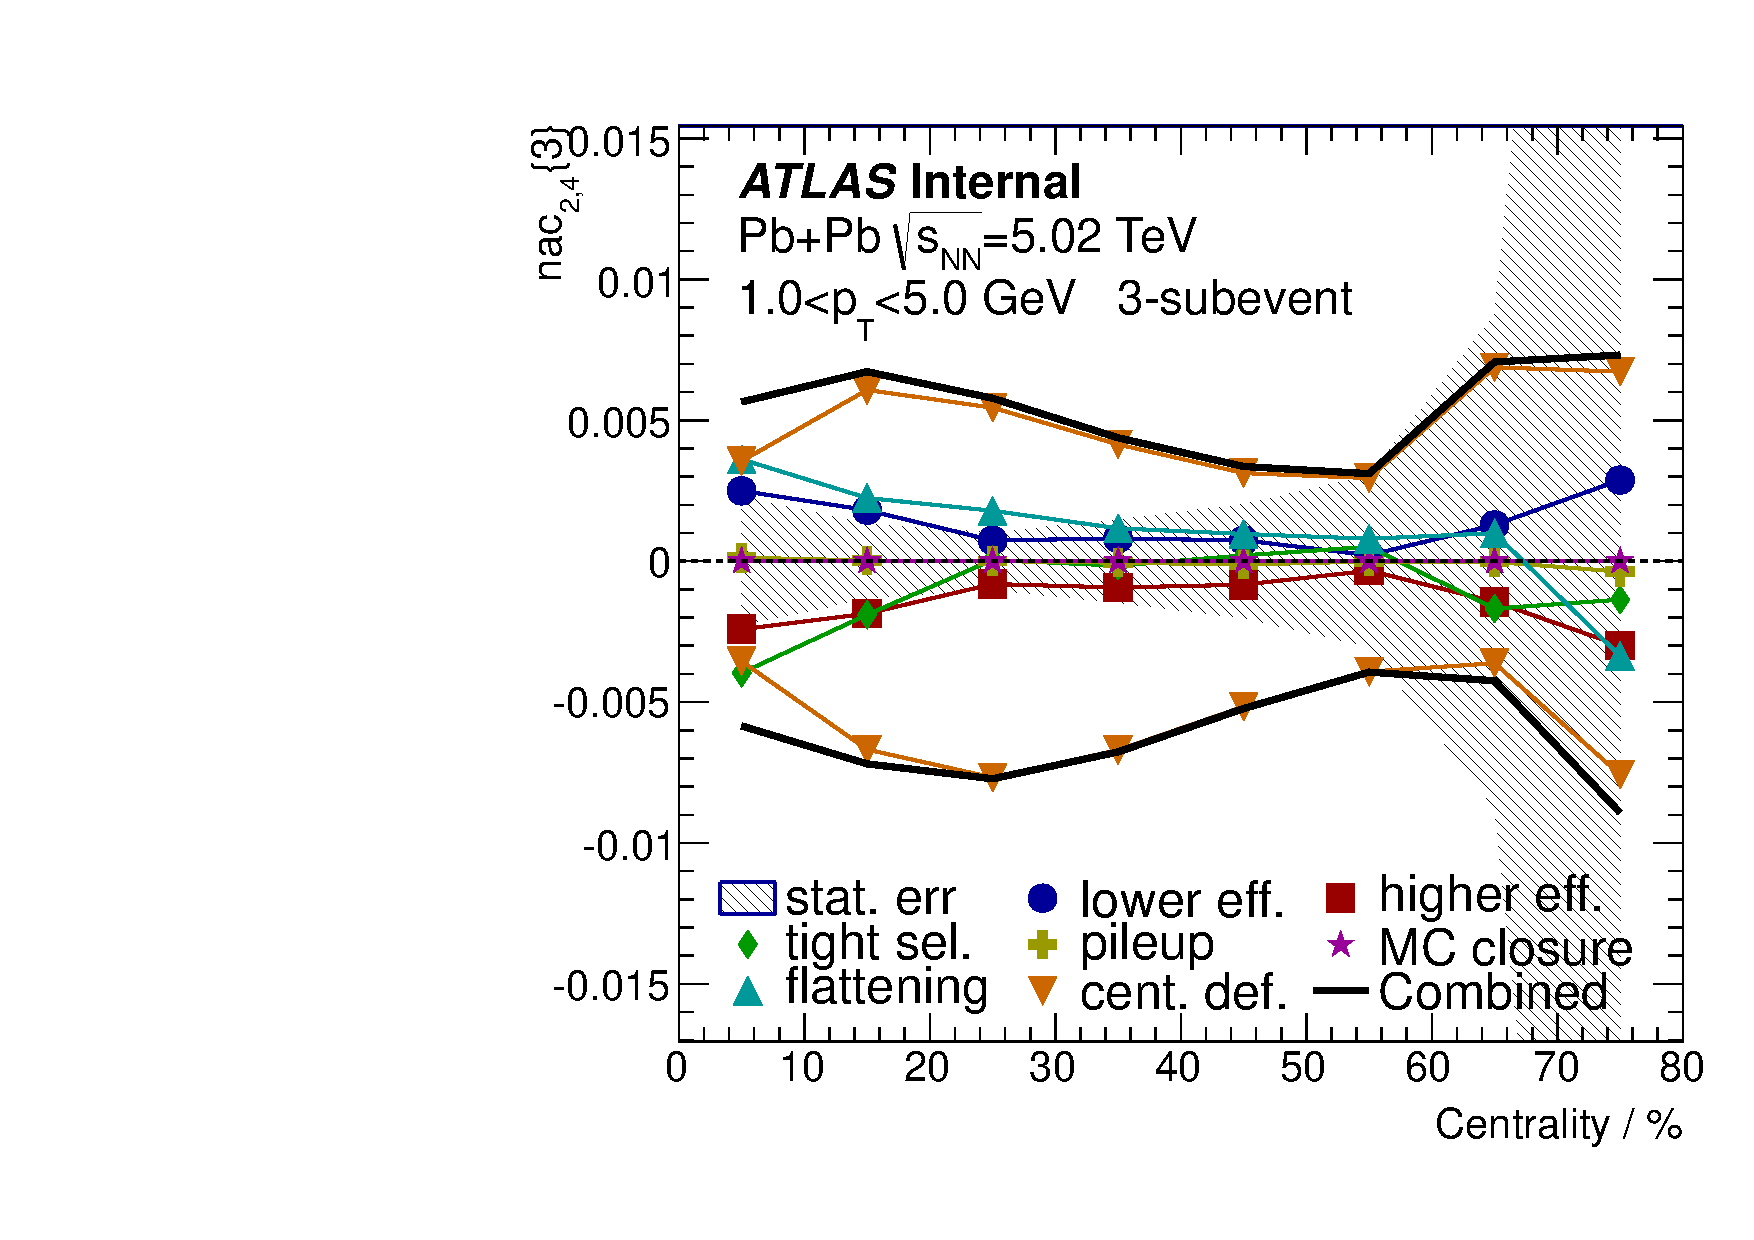
\includegraphics[width=.425\linewidth]{figs/sec_sys/summary/sys_nac_3sub_Har2_Pt1.pdf}
\caption{Breakdown of systematics for normalized symmetric and asymmetric cumulants, using 3-subevent method, with low (left) and high (right) $p_\text{T}$ ranges. Different rows are for different harmonics.}
\label{fig:apdx_sys_nsc_3sub}
\end{figure}



\subsection{Results for 2.76 TeV Pb+Pb}

\begin{figure}[H]
\centering
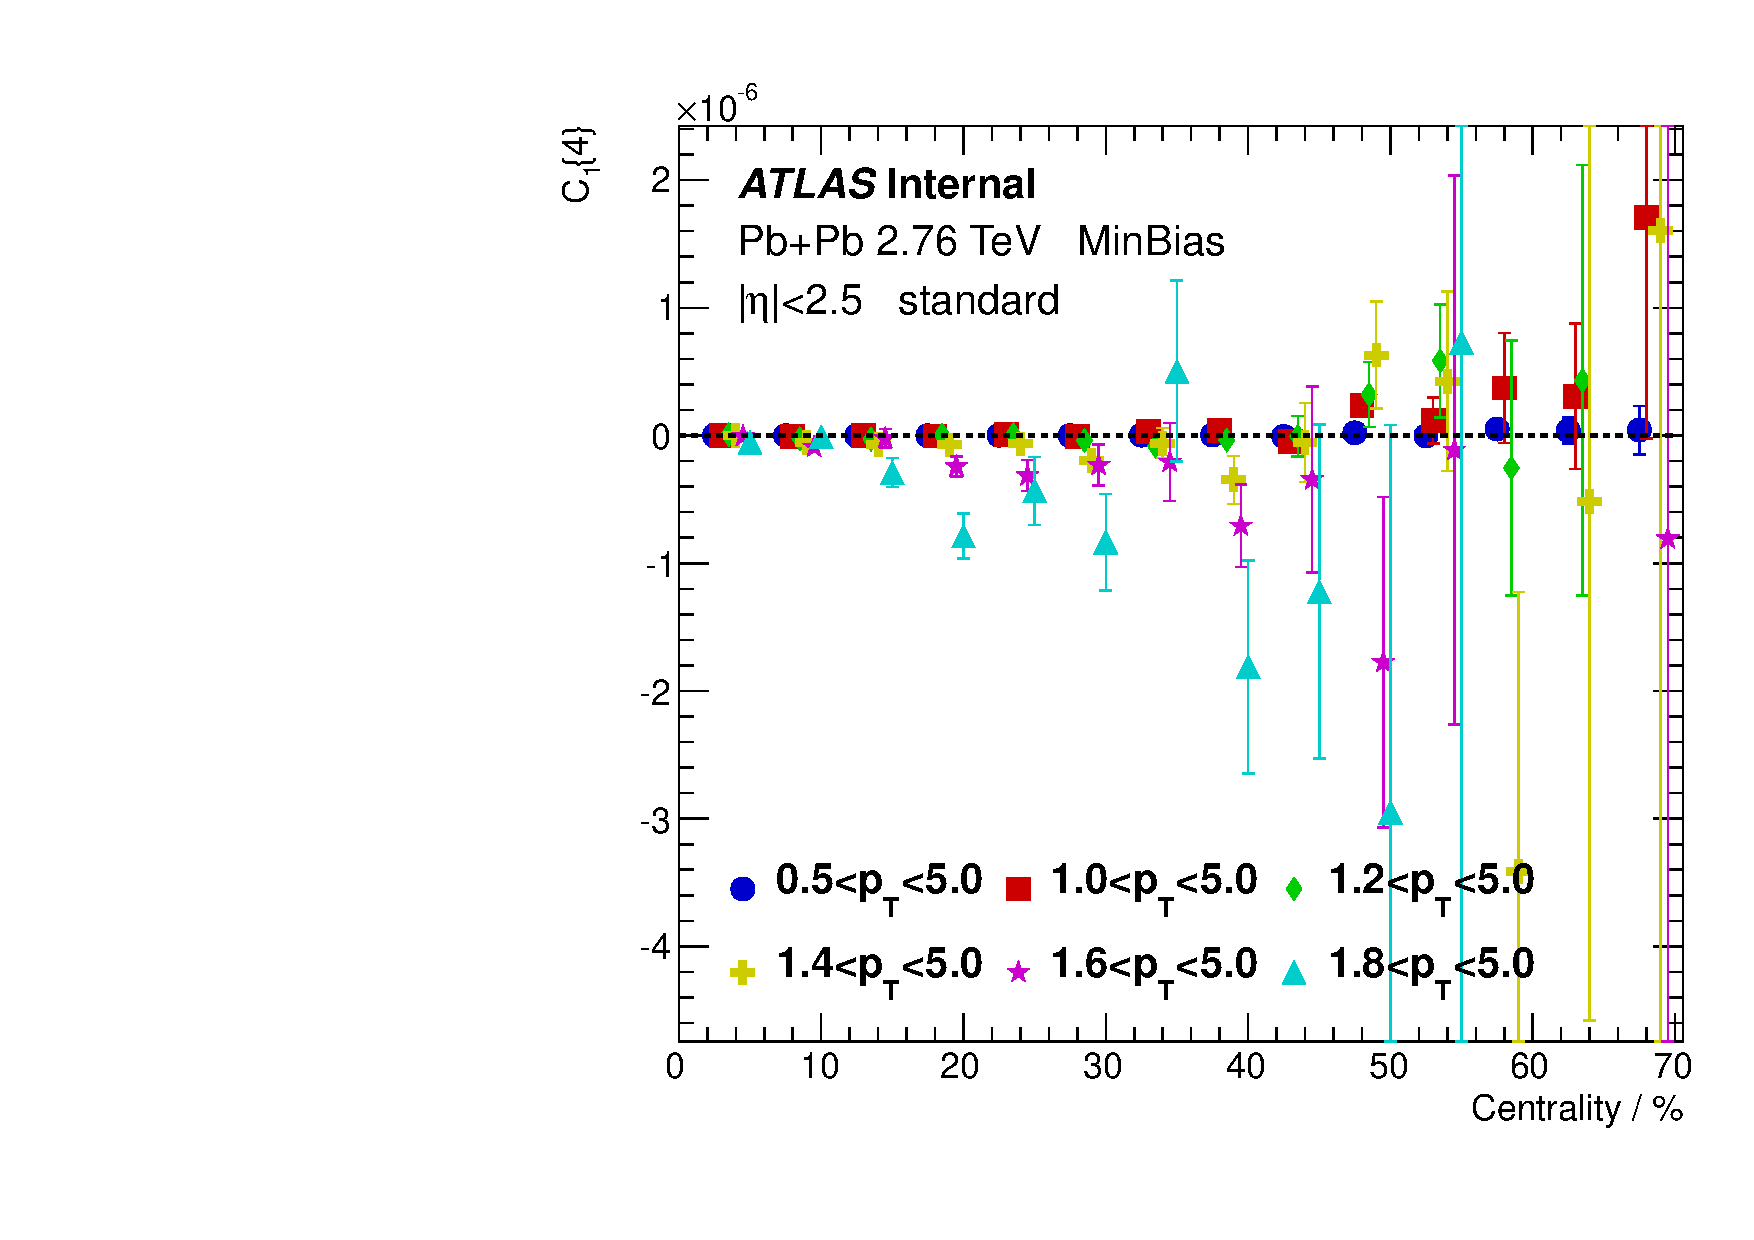
\includegraphics[width=.245\linewidth]{figs/sec_appendix/PbPb276/PbPb276_pT_1sub_Har1.pdf}
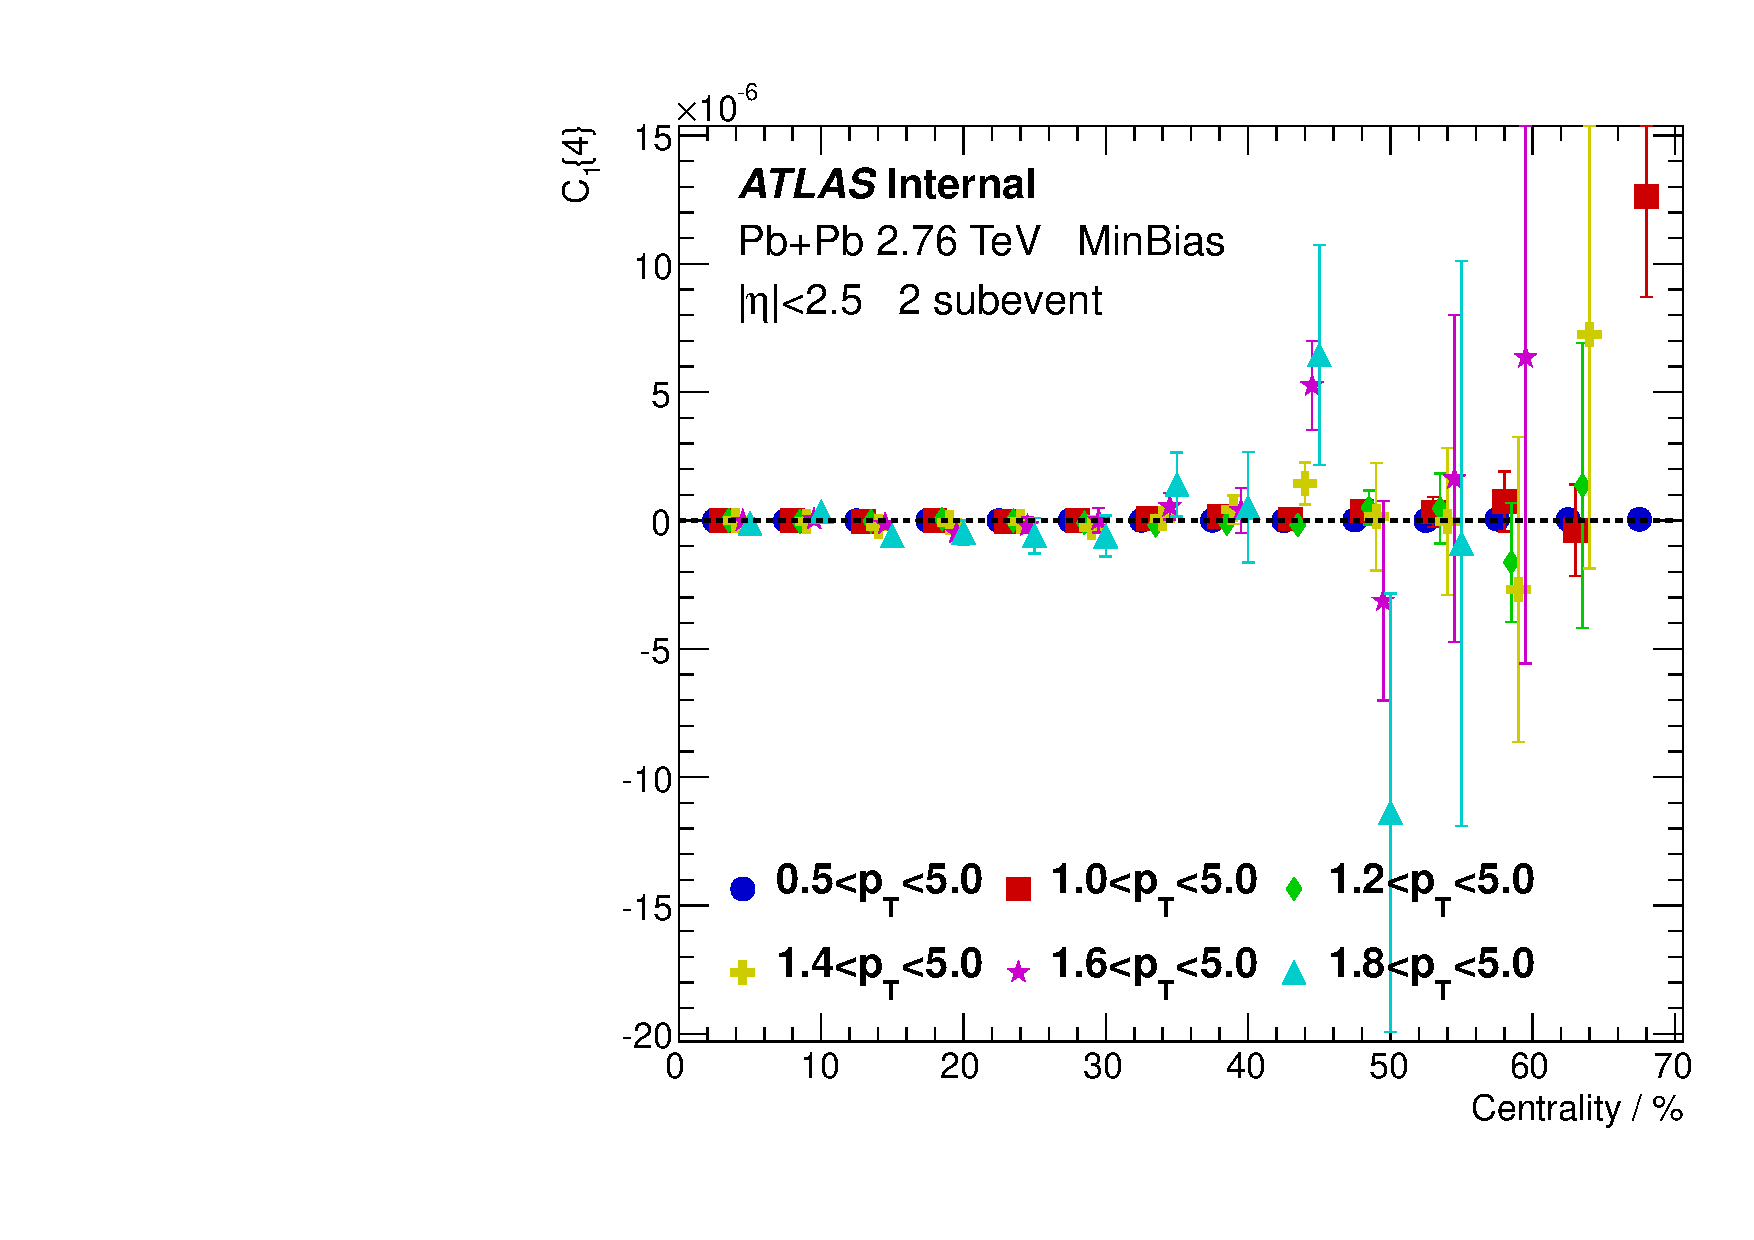
\includegraphics[width=.245\linewidth]{figs/sec_appendix/PbPb276/PbPb276_pT_2sub_Har1.pdf}
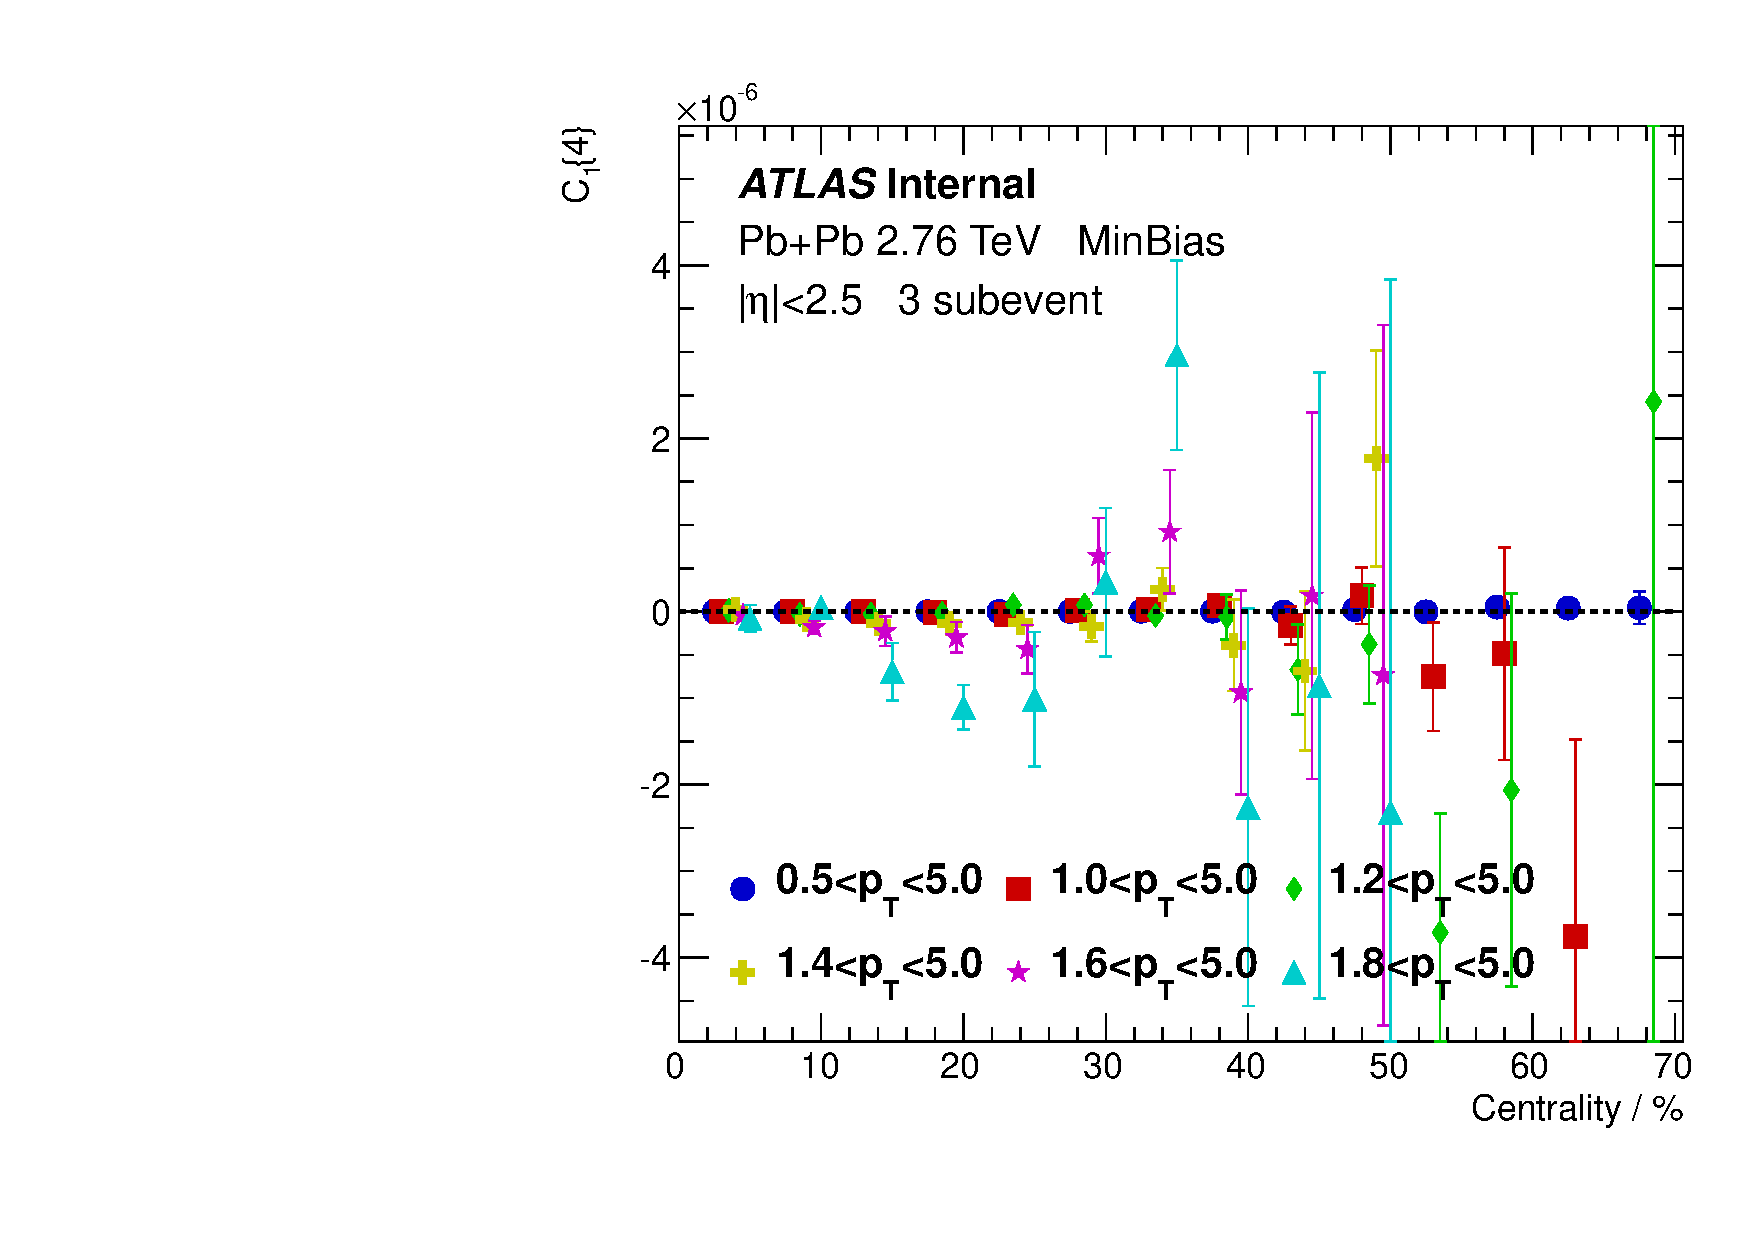
\includegraphics[width=.245\linewidth]{figs/sec_appendix/PbPb276/PbPb276_pT_3sub_Har1.pdf}
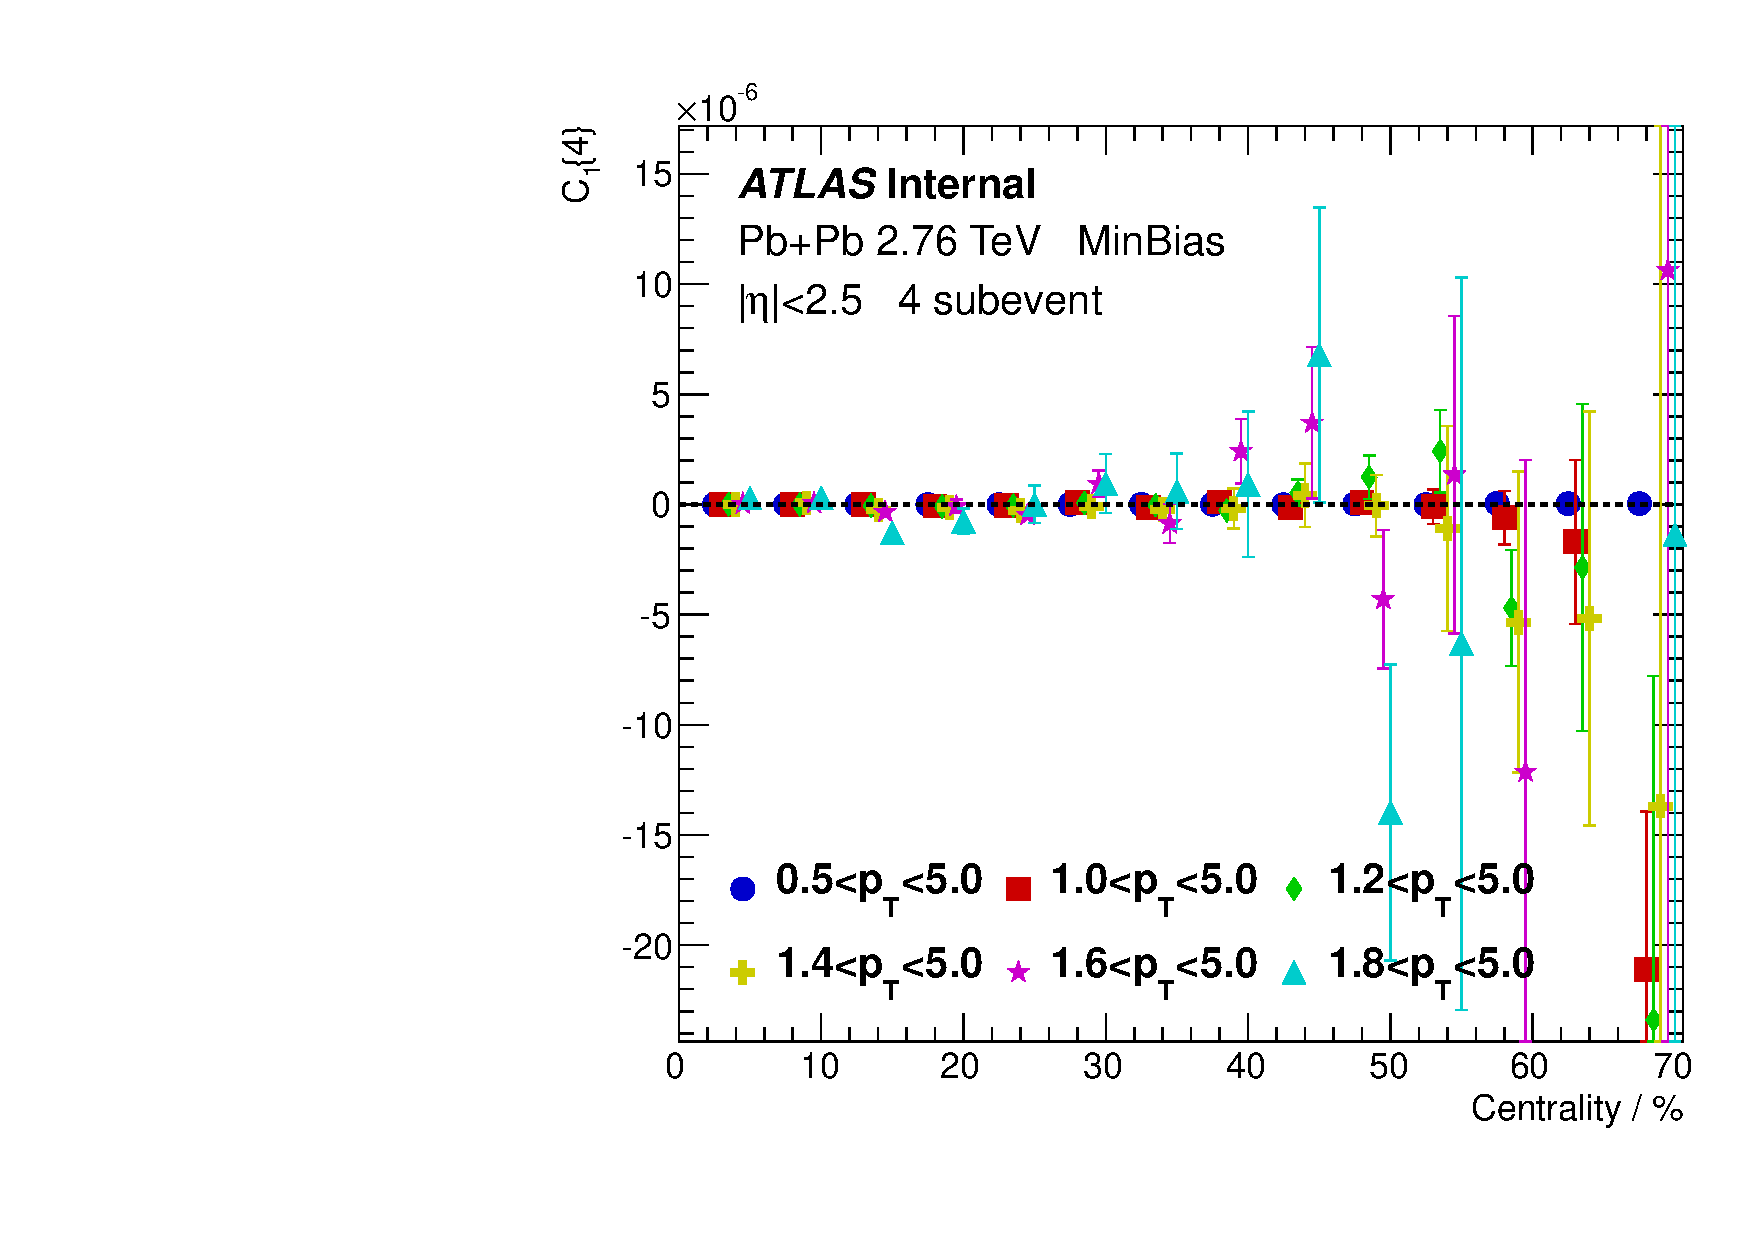
\includegraphics[width=.245\linewidth]{figs/sec_appendix/PbPb276/PbPb276_pT_4sub_Har1.pdf}
\caption{$c_1\{4\}$ in 2.76 TeV Pb+Pb, calculated in different $p_\text{T}$ ranges. Each panel is for each cumulant method.}
\label{fig:PbPb276_pT_v1}
\end{figure}

\begin{figure}[H]
\centering
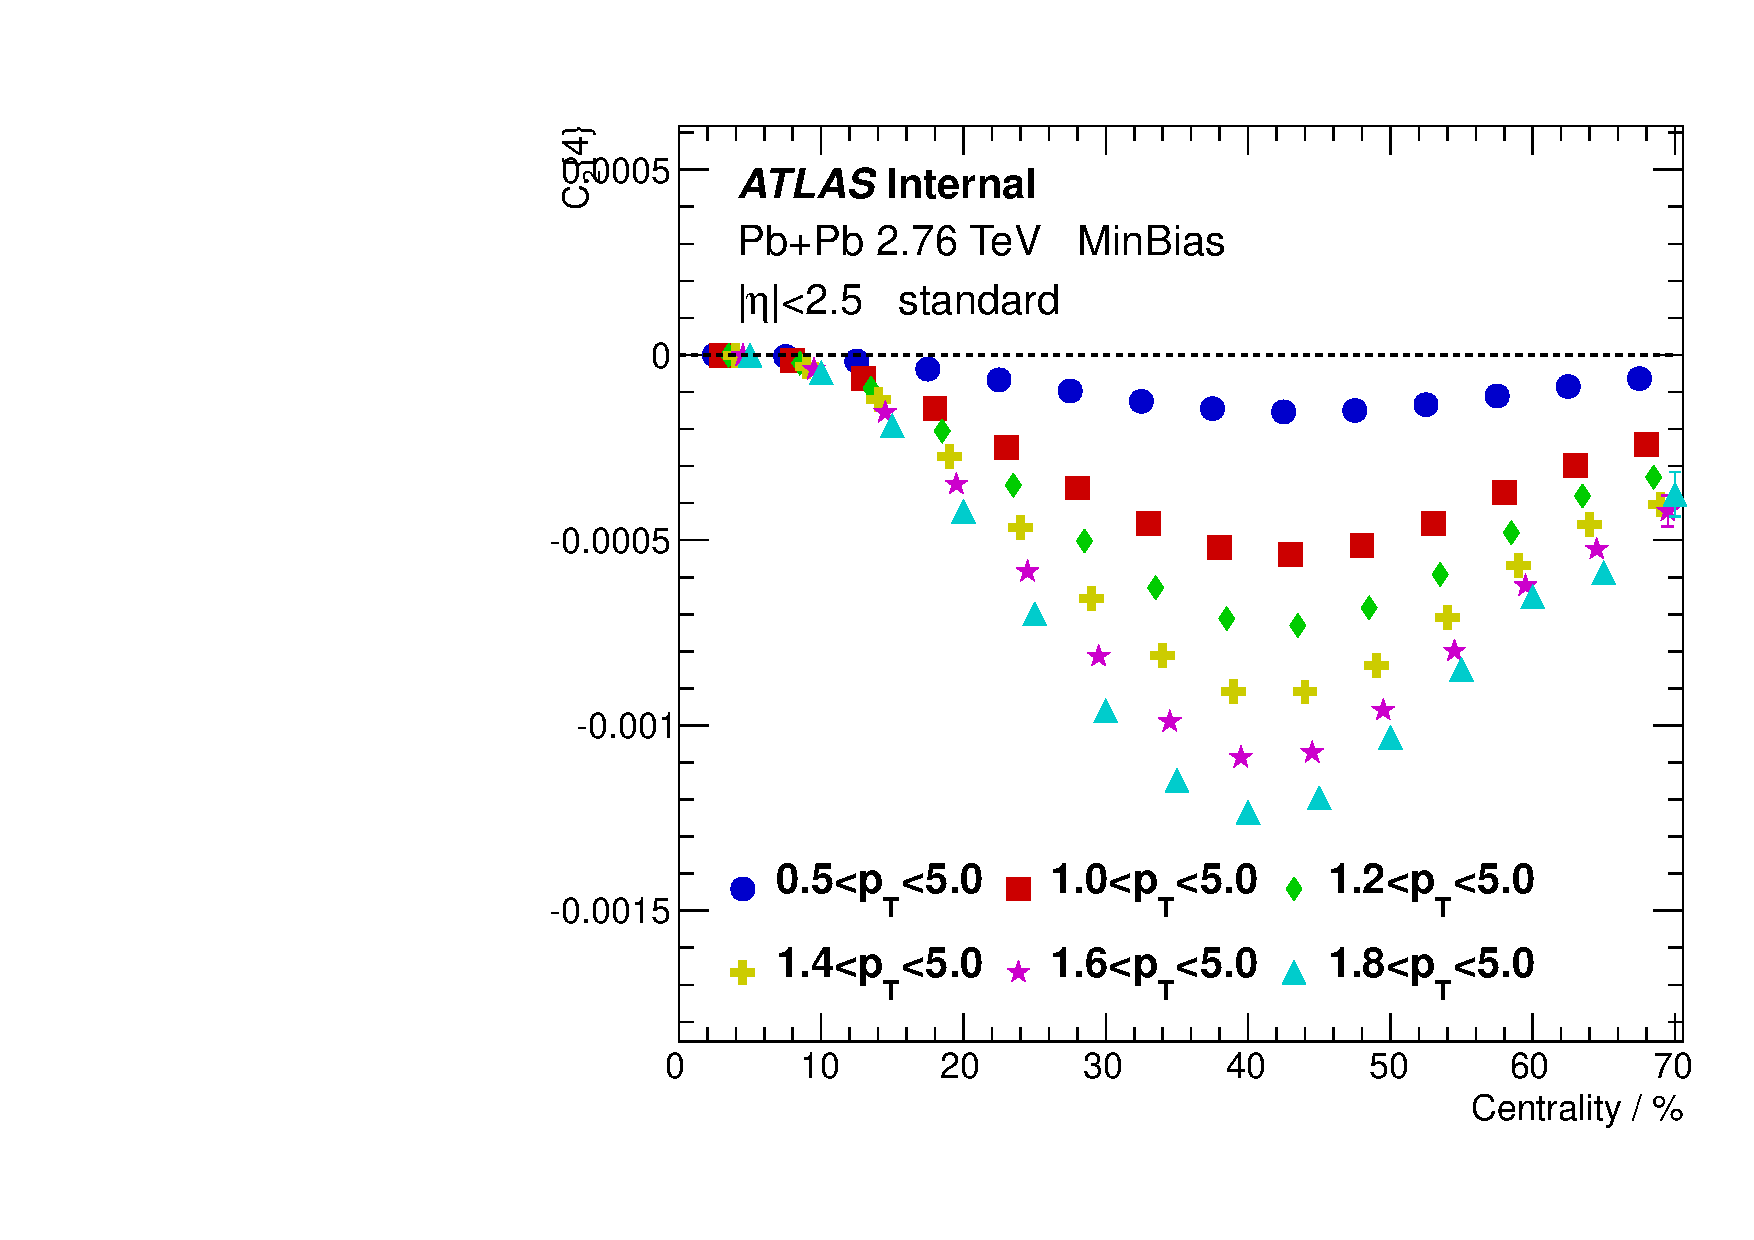
\includegraphics[width=.245\linewidth]{figs/sec_appendix/PbPb276/PbPb276_pT_1sub_Har2.pdf}
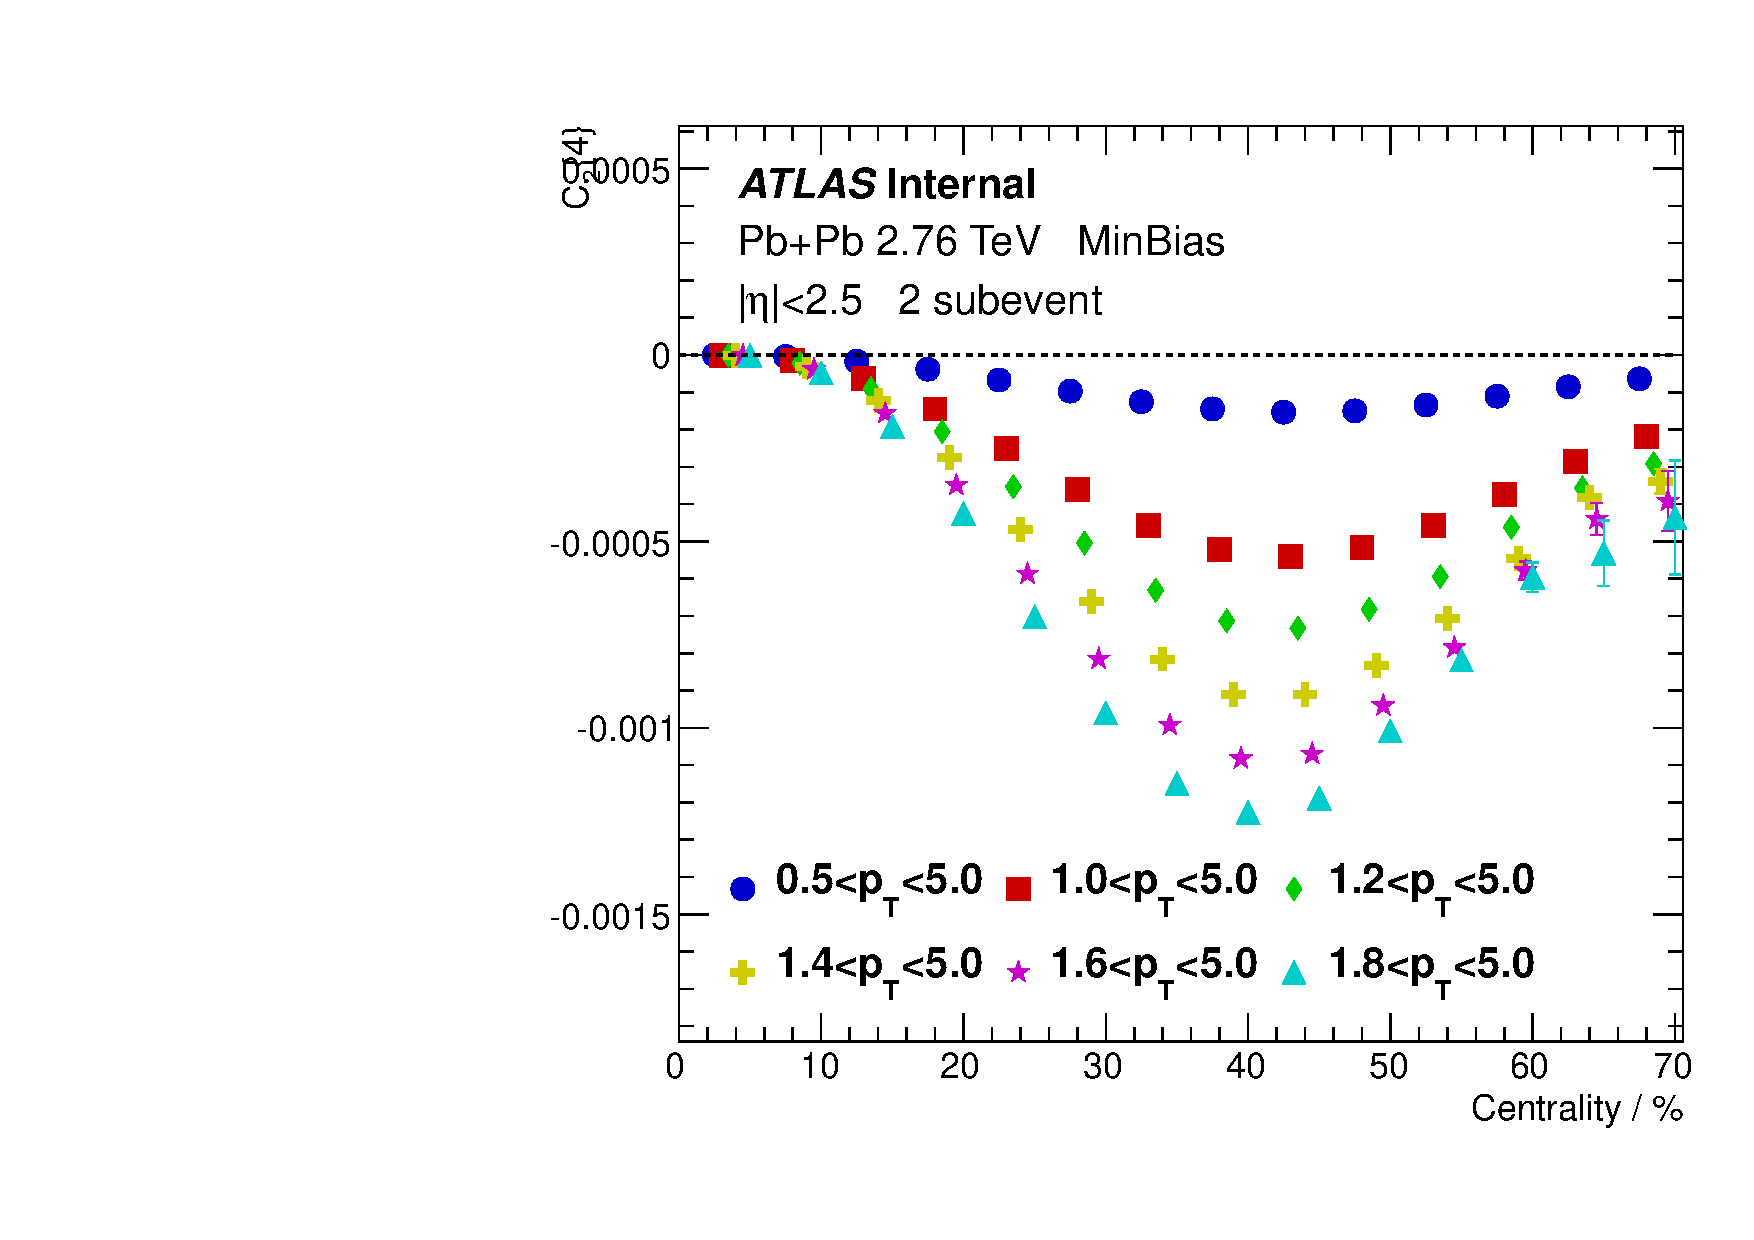
\includegraphics[width=.245\linewidth]{figs/sec_appendix/PbPb276/PbPb276_pT_2sub_Har2.pdf}
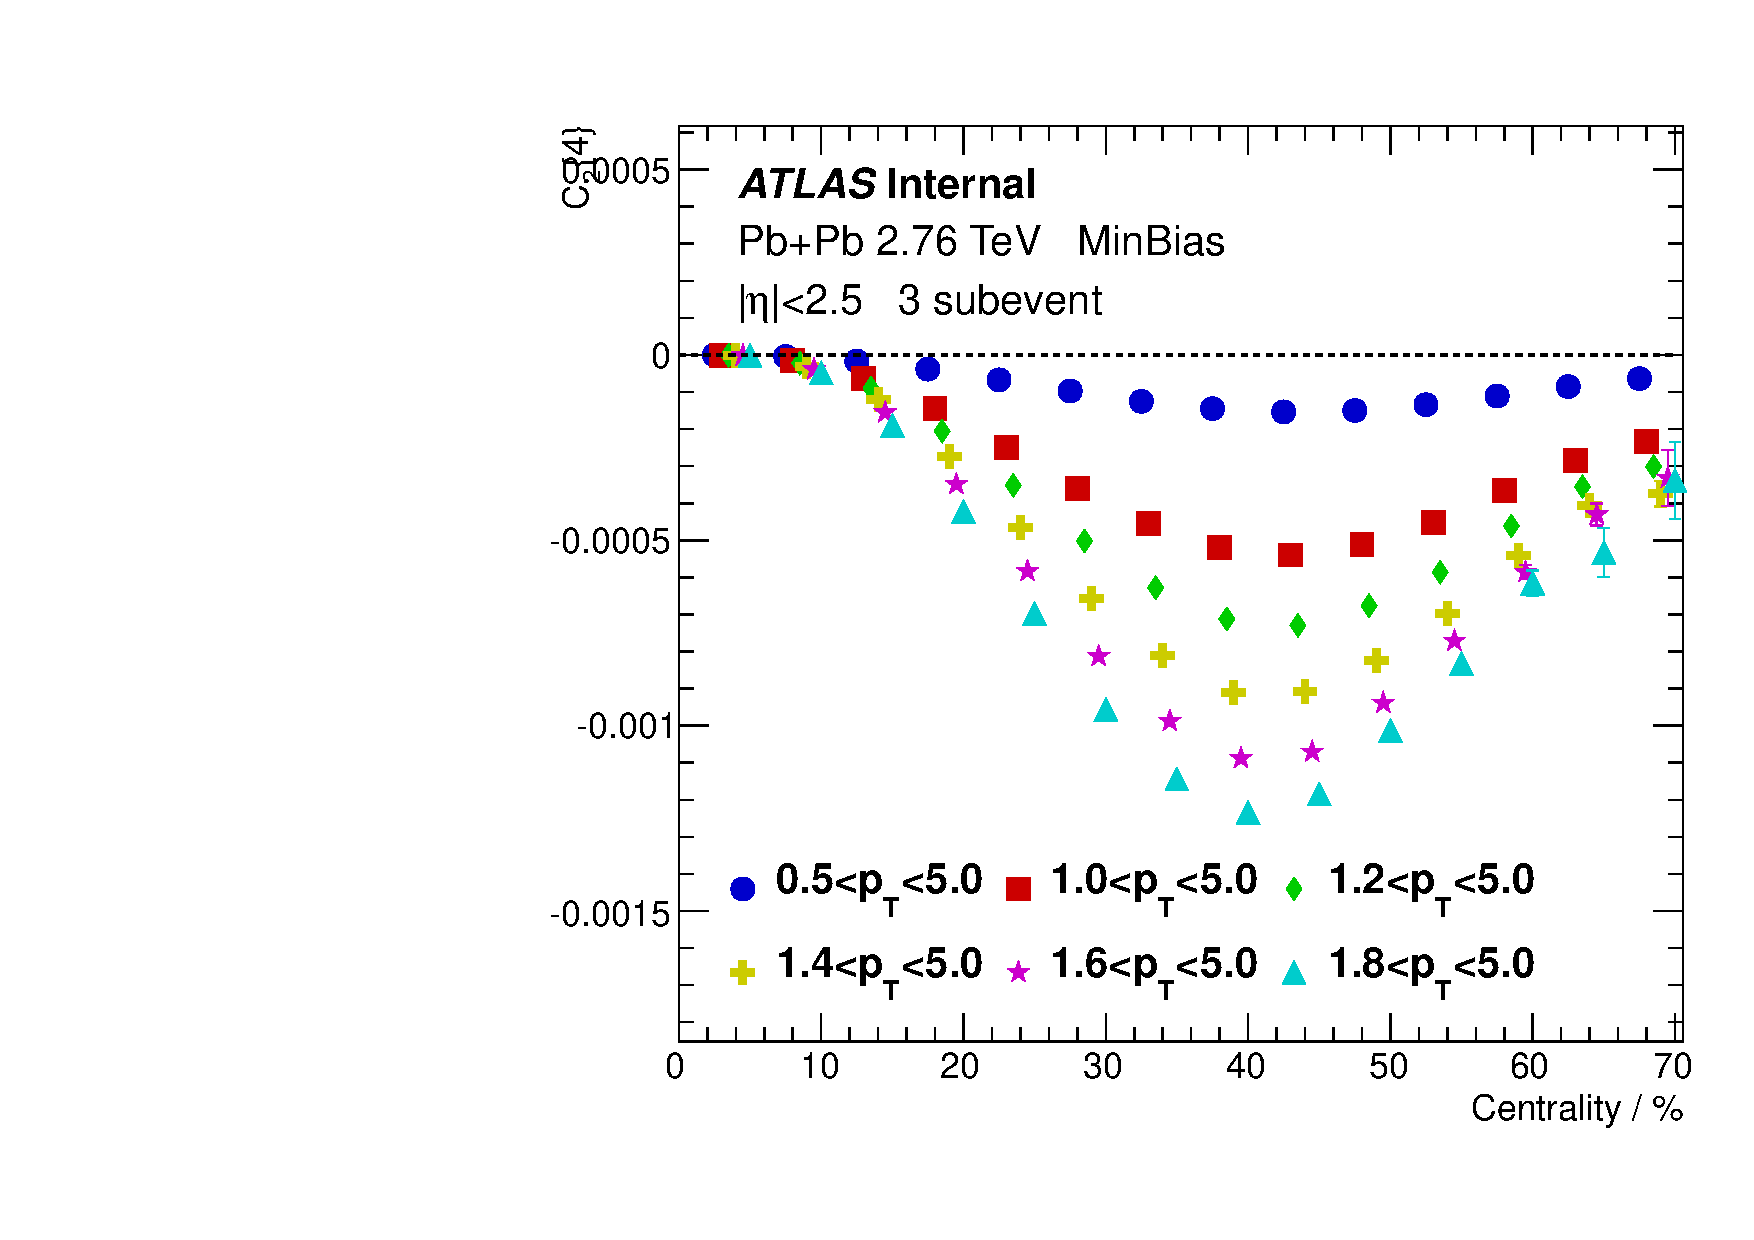
\includegraphics[width=.245\linewidth]{figs/sec_appendix/PbPb276/PbPb276_pT_3sub_Har2.pdf}
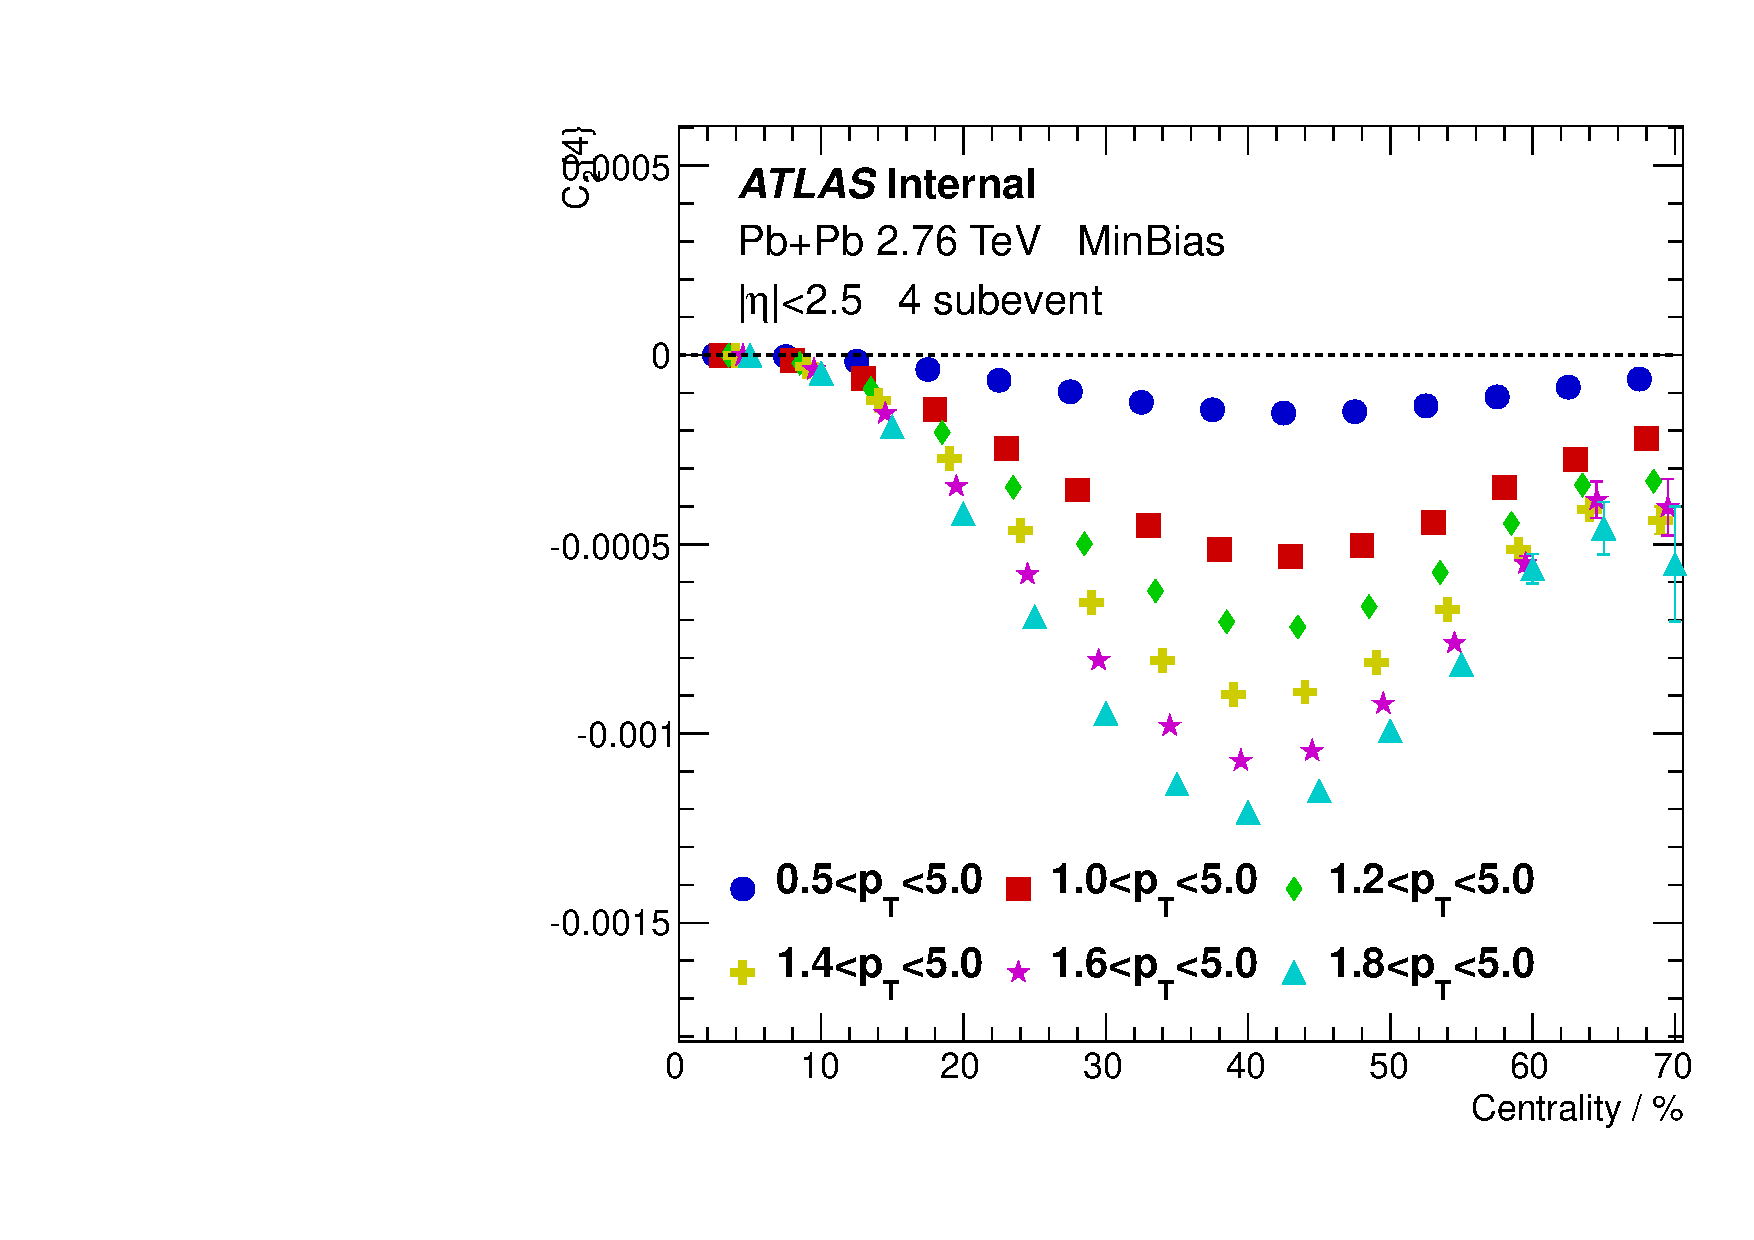
\includegraphics[width=.245\linewidth]{figs/sec_appendix/PbPb276/PbPb276_pT_4sub_Har2.pdf}
\caption{$c_2\{4\}$ in 2.76 TeV Pb+Pb, calculated in different $p_\text{T}$ ranges. Each panel is for each cumulant method.}
\label{fig:PbPb276_pT_v2}
\end{figure}

\begin{figure}[H]
\centering
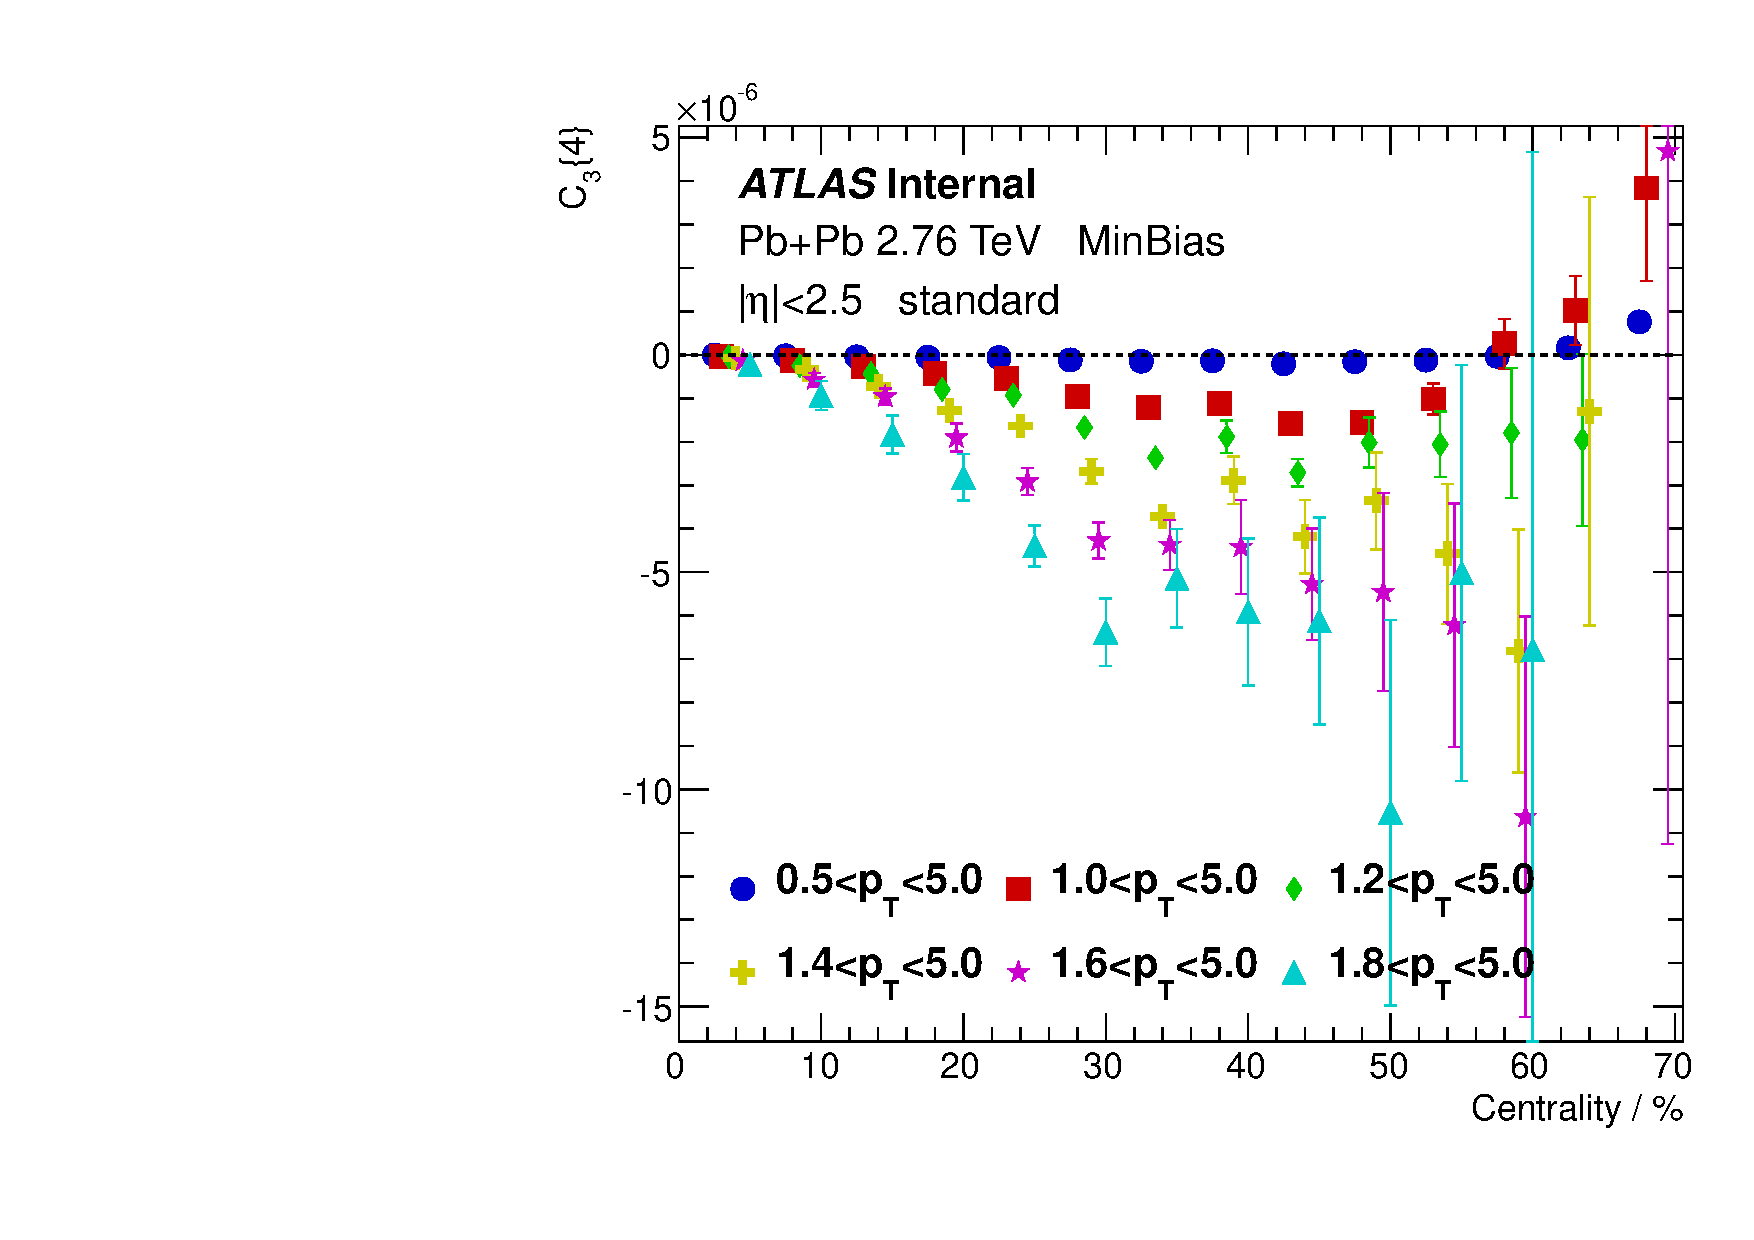
\includegraphics[width=.245\linewidth]{figs/sec_appendix/PbPb276/PbPb276_pT_1sub_Har3.pdf}
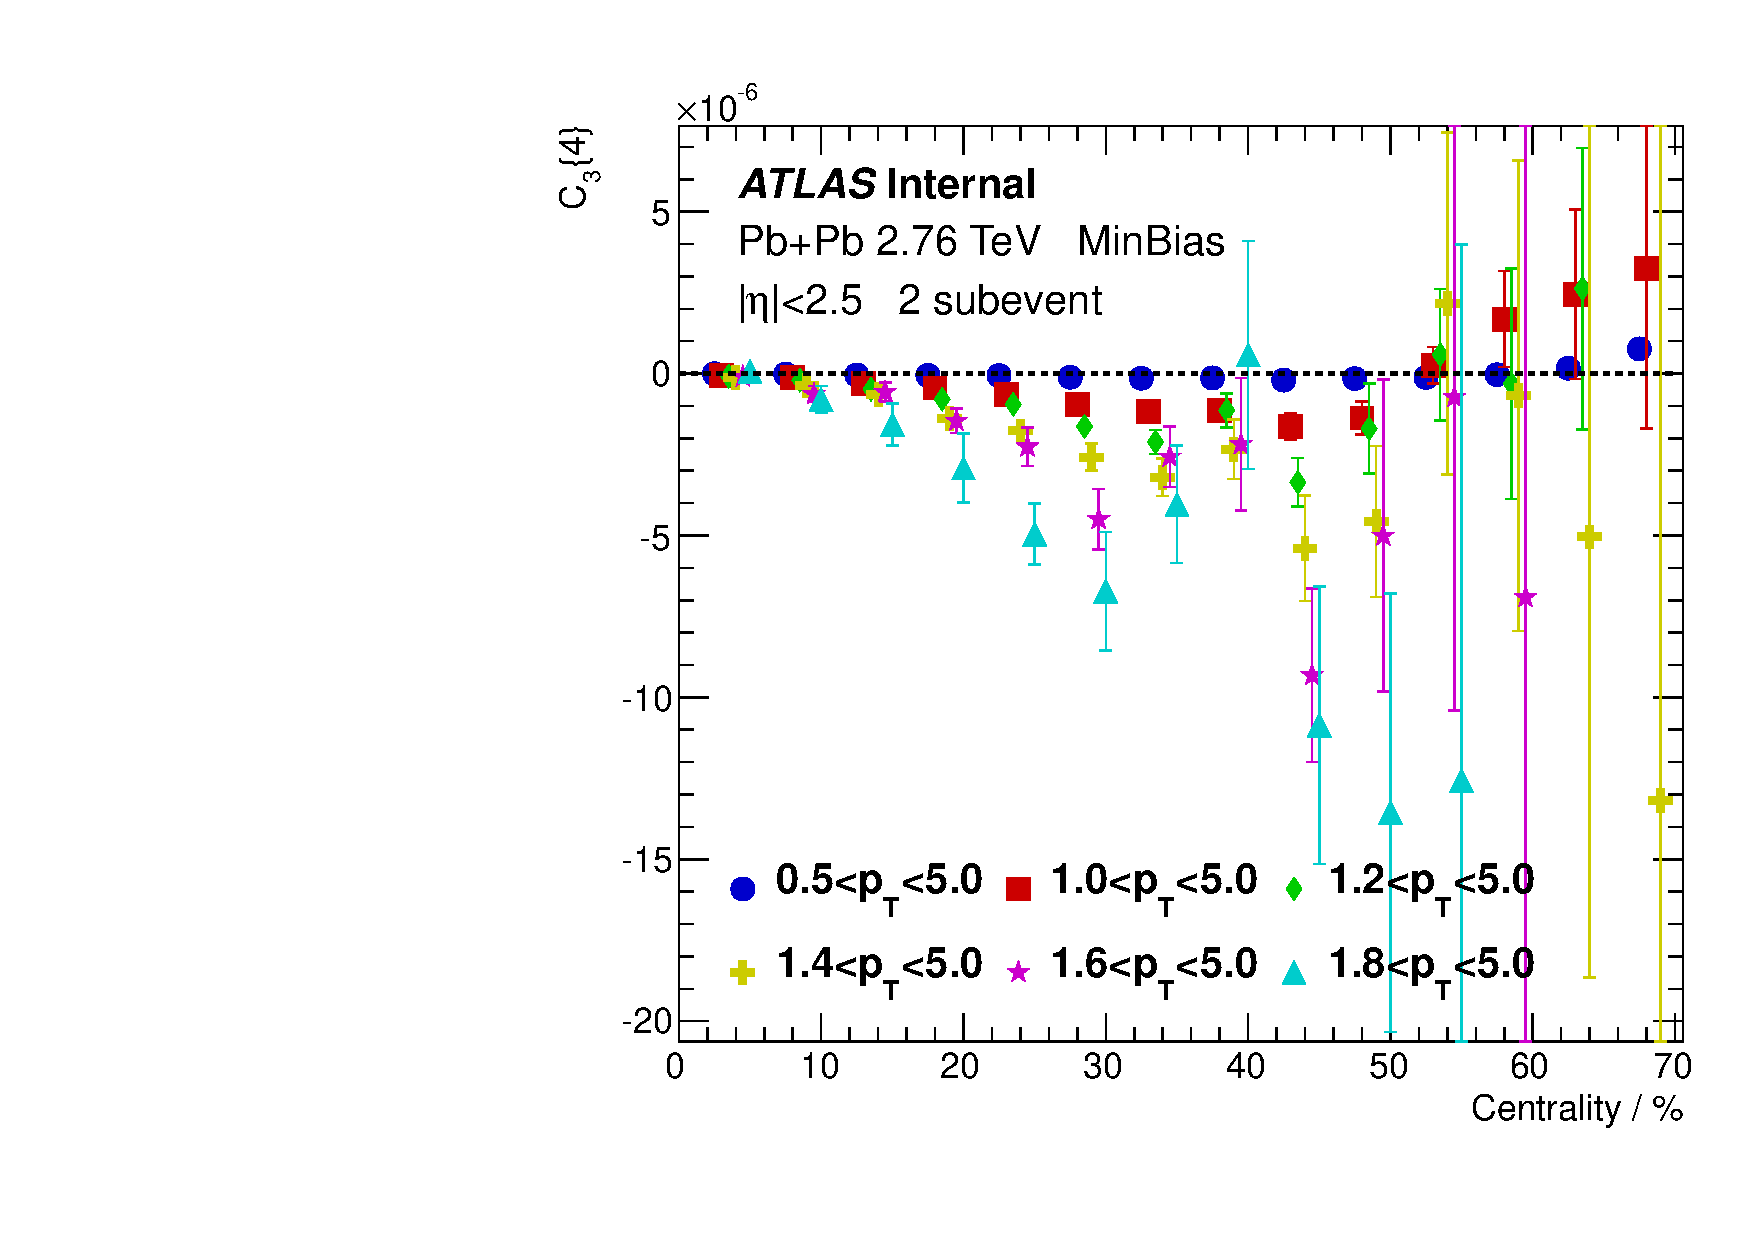
\includegraphics[width=.245\linewidth]{figs/sec_appendix/PbPb276/PbPb276_pT_2sub_Har3.pdf}
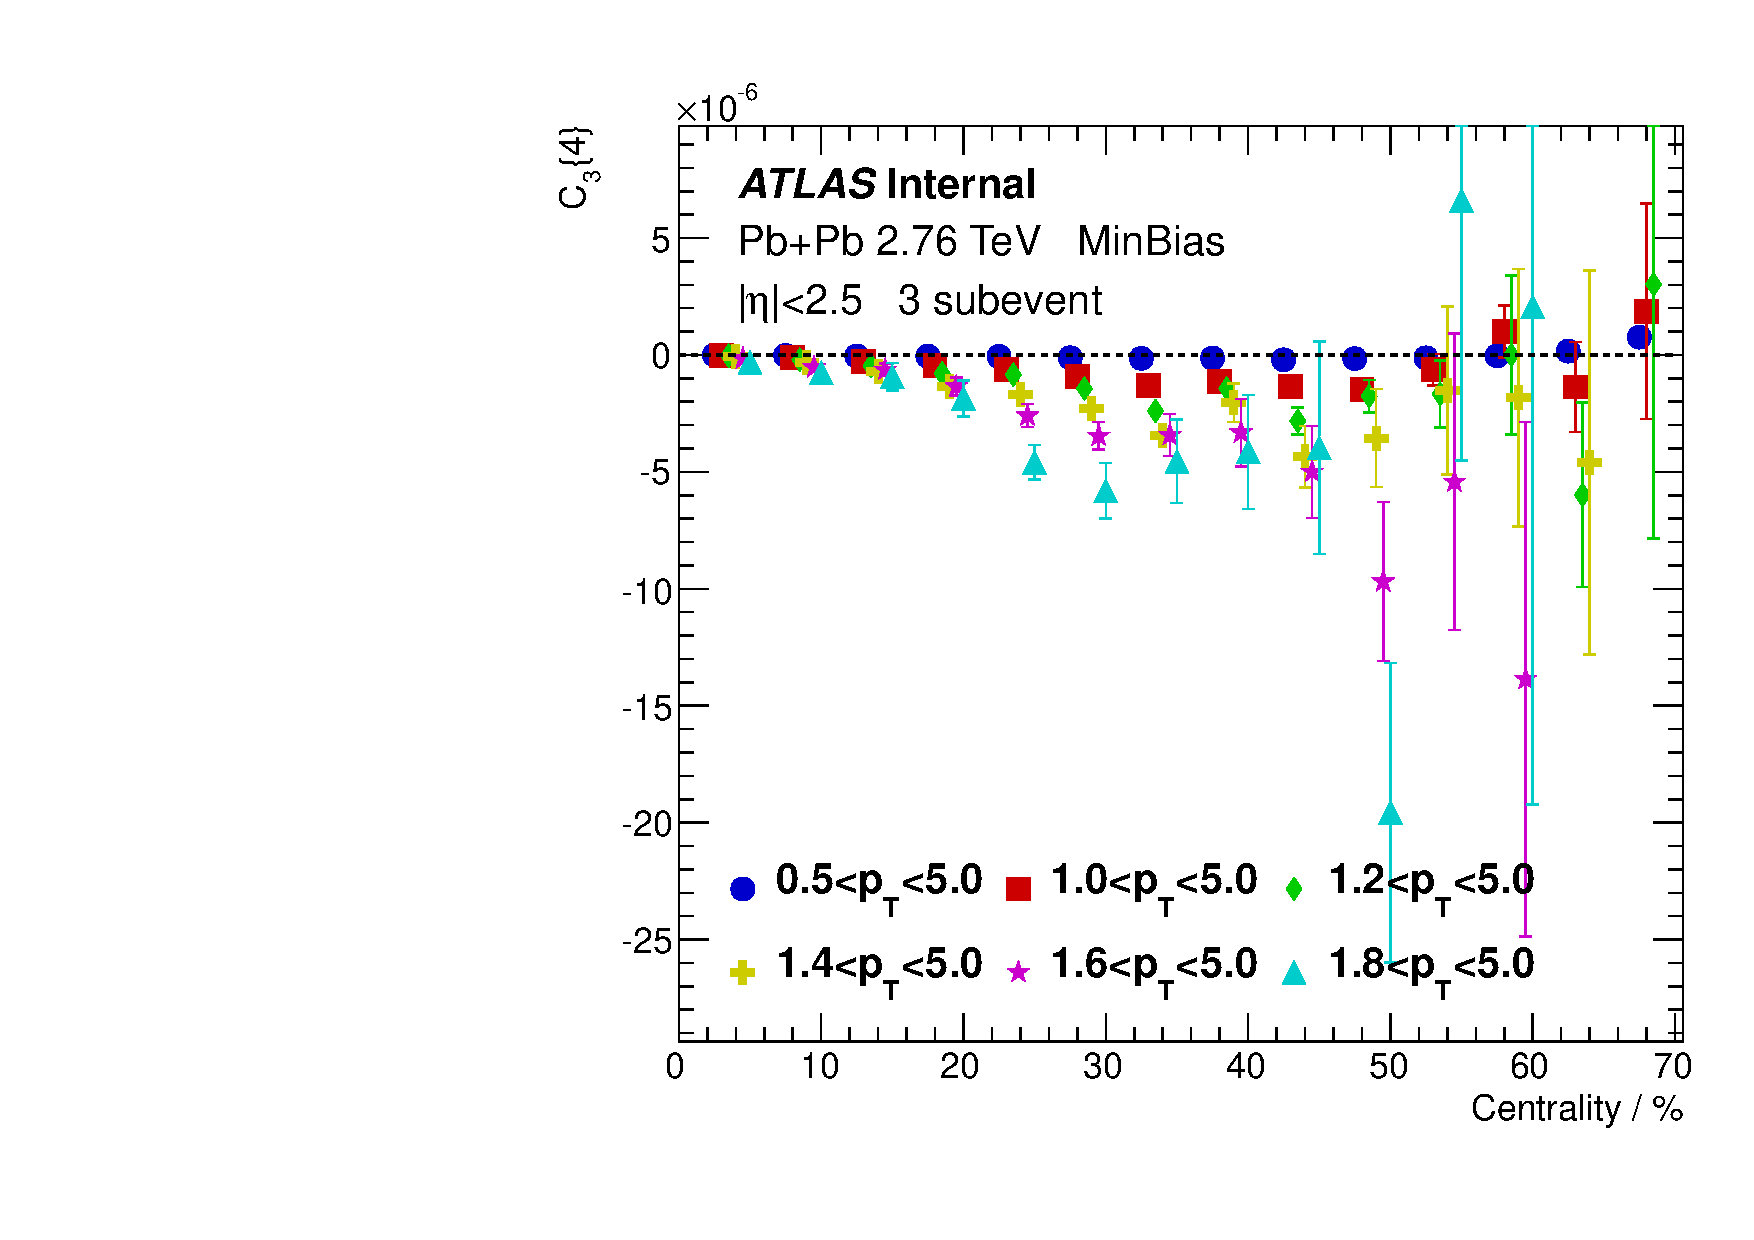
\includegraphics[width=.245\linewidth]{figs/sec_appendix/PbPb276/PbPb276_pT_3sub_Har3.pdf}
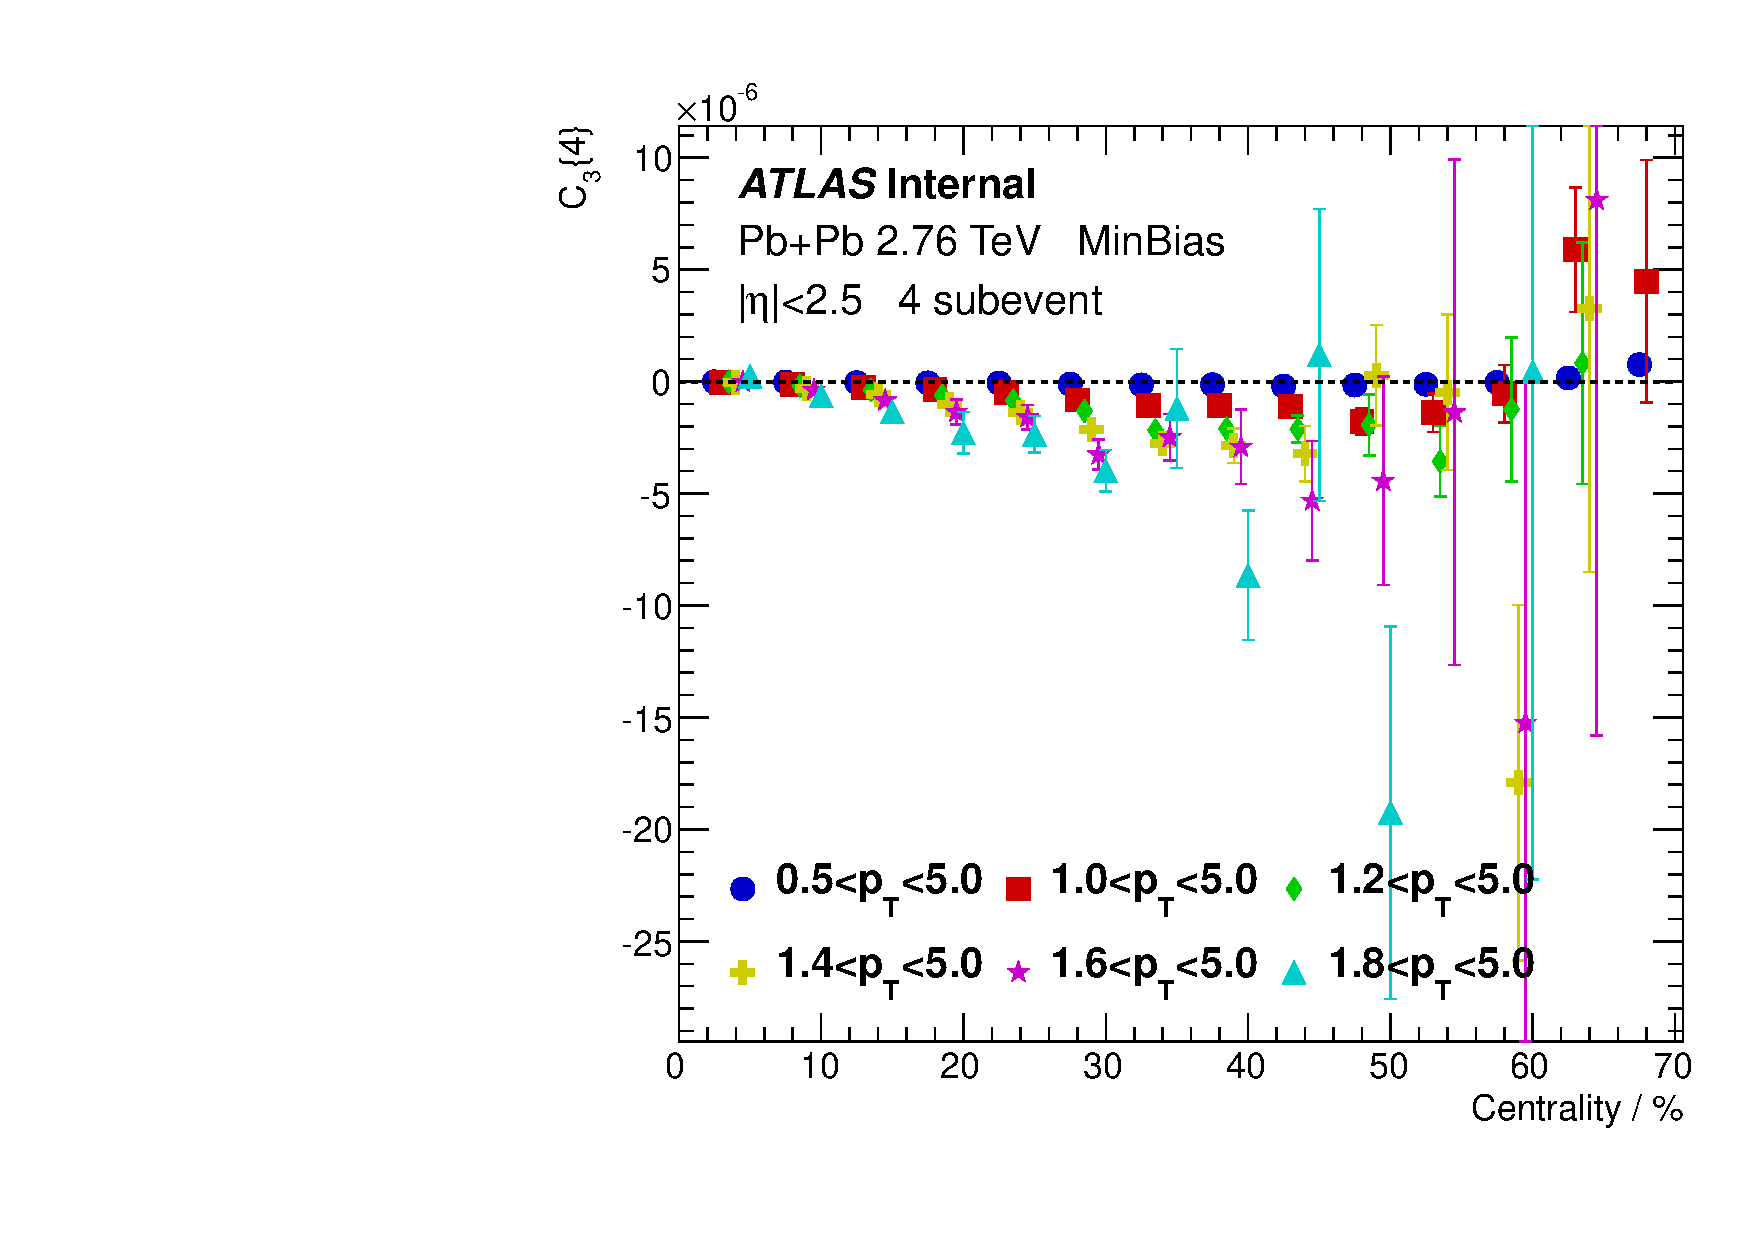
\includegraphics[width=.245\linewidth]{figs/sec_appendix/PbPb276/PbPb276_pT_4sub_Har3.pdf}
\caption{$c_3\{4\}$ in 2.76 TeV Pb+Pb, calculated in different $p_\text{T}$ ranges. Each panel is for each cumulant method.}
\label{fig:PbPb276_pT_v3}
\end{figure}

\begin{figure}[H]
\centering
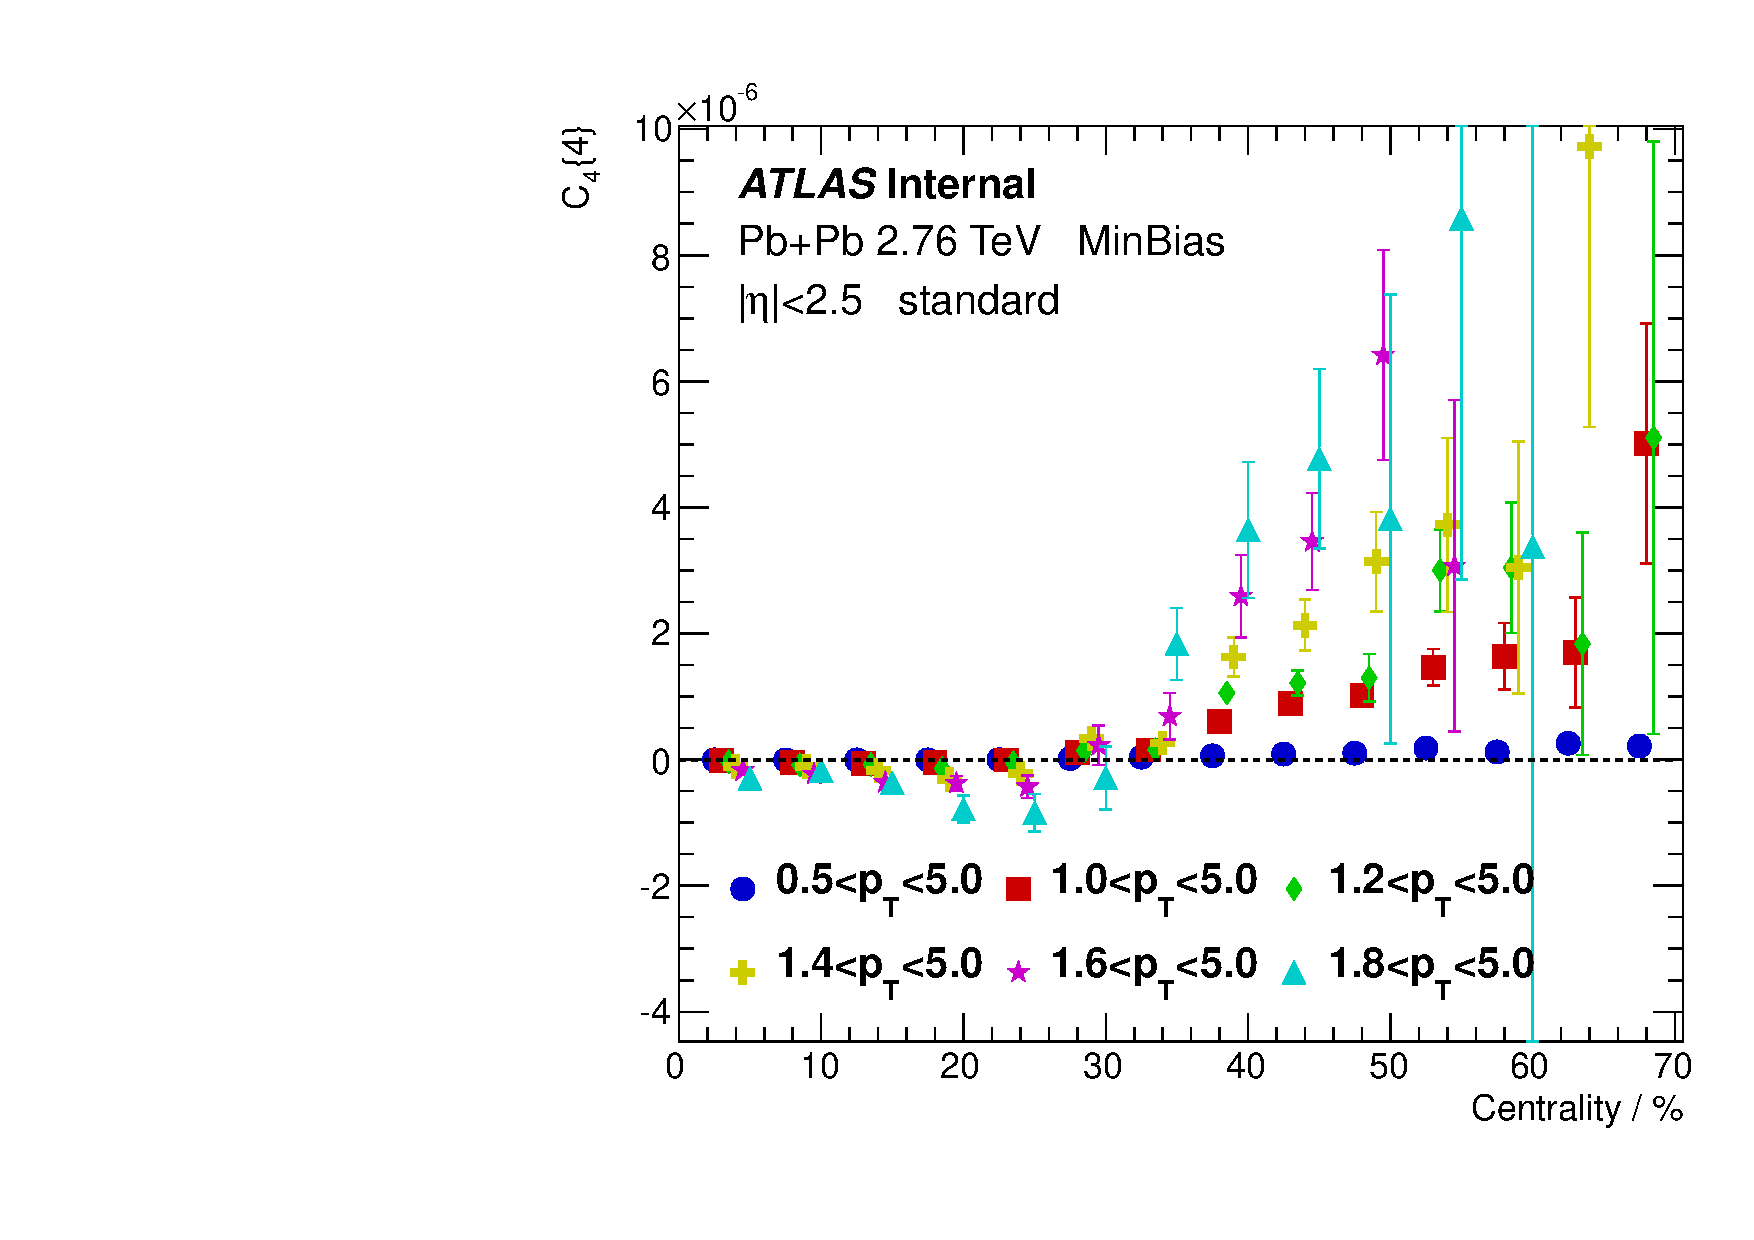
\includegraphics[width=.245\linewidth]{figs/sec_appendix/PbPb276/PbPb276_pT_1sub_Har4.pdf}
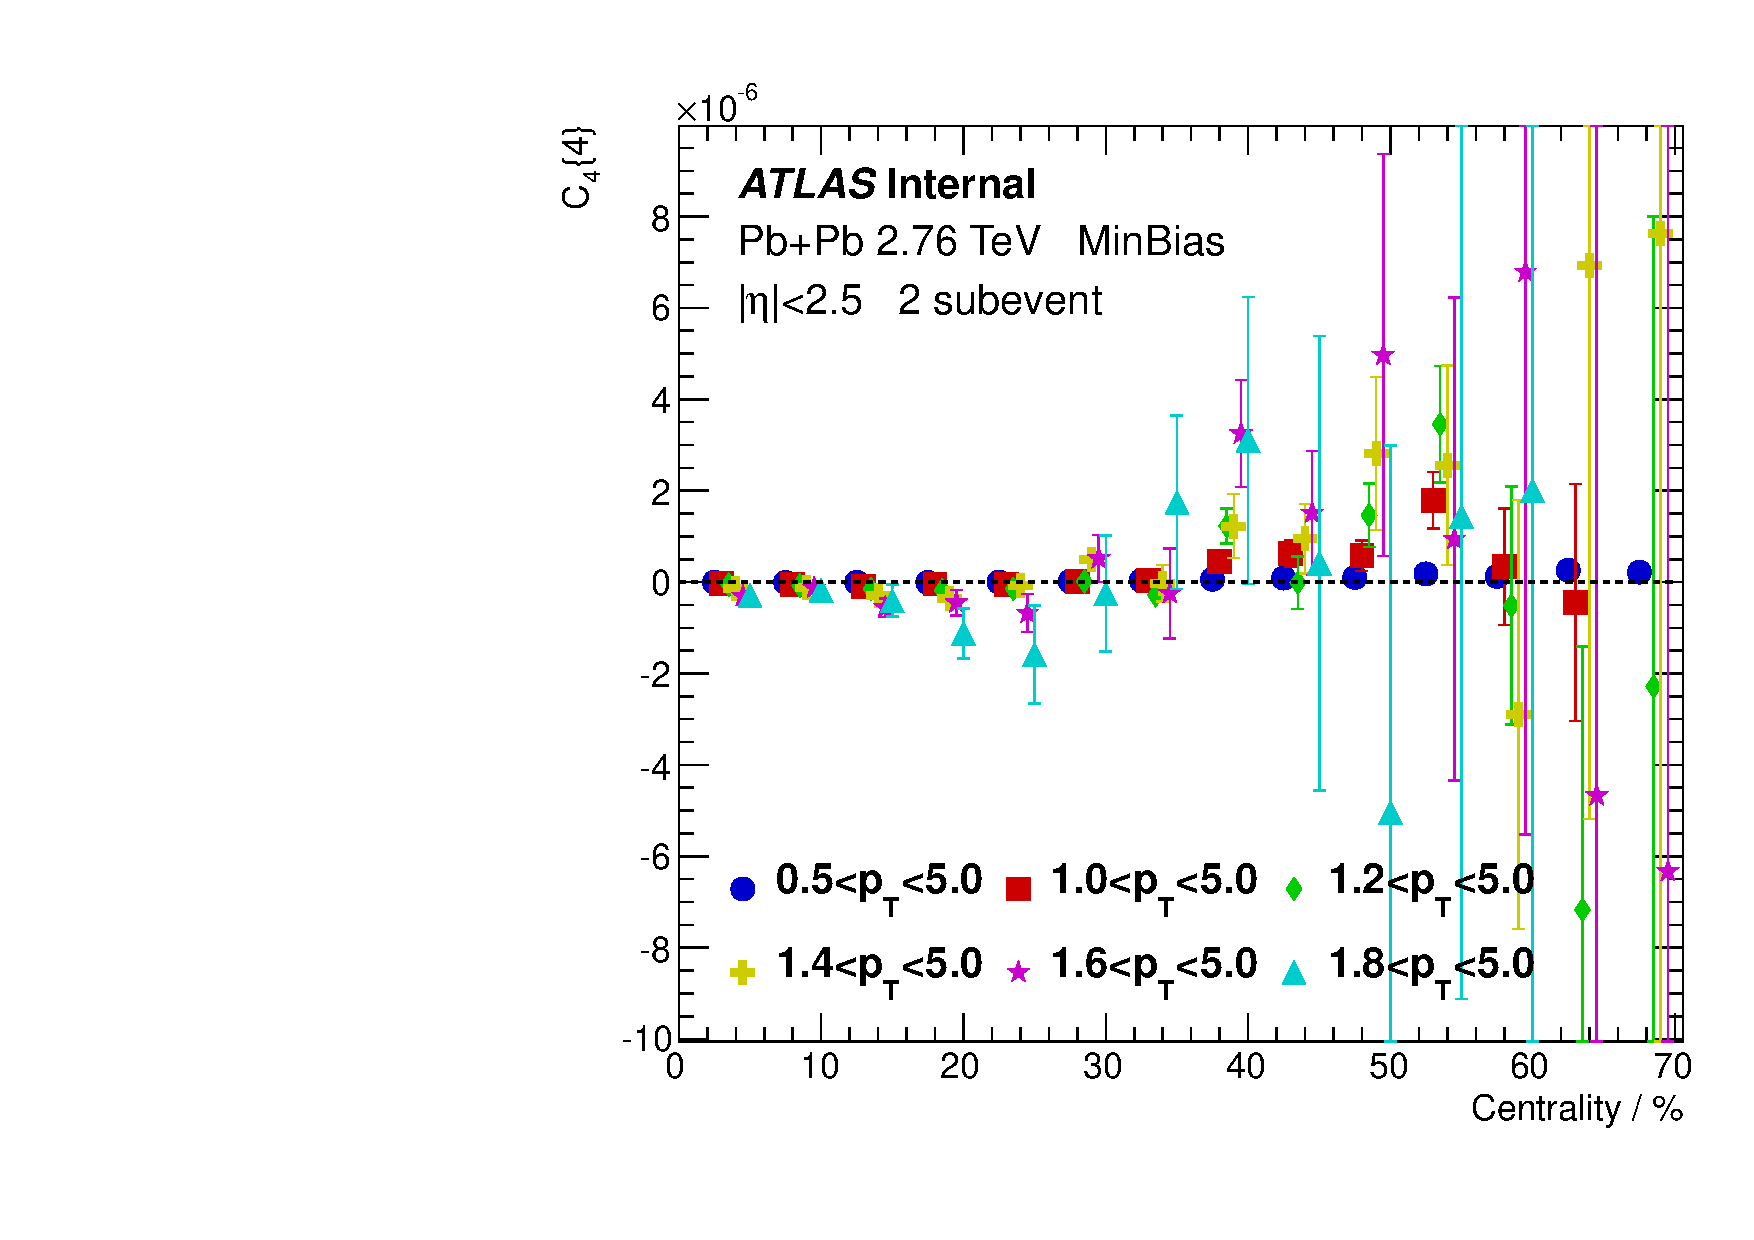
\includegraphics[width=.245\linewidth]{figs/sec_appendix/PbPb276/PbPb276_pT_2sub_Har4.pdf}
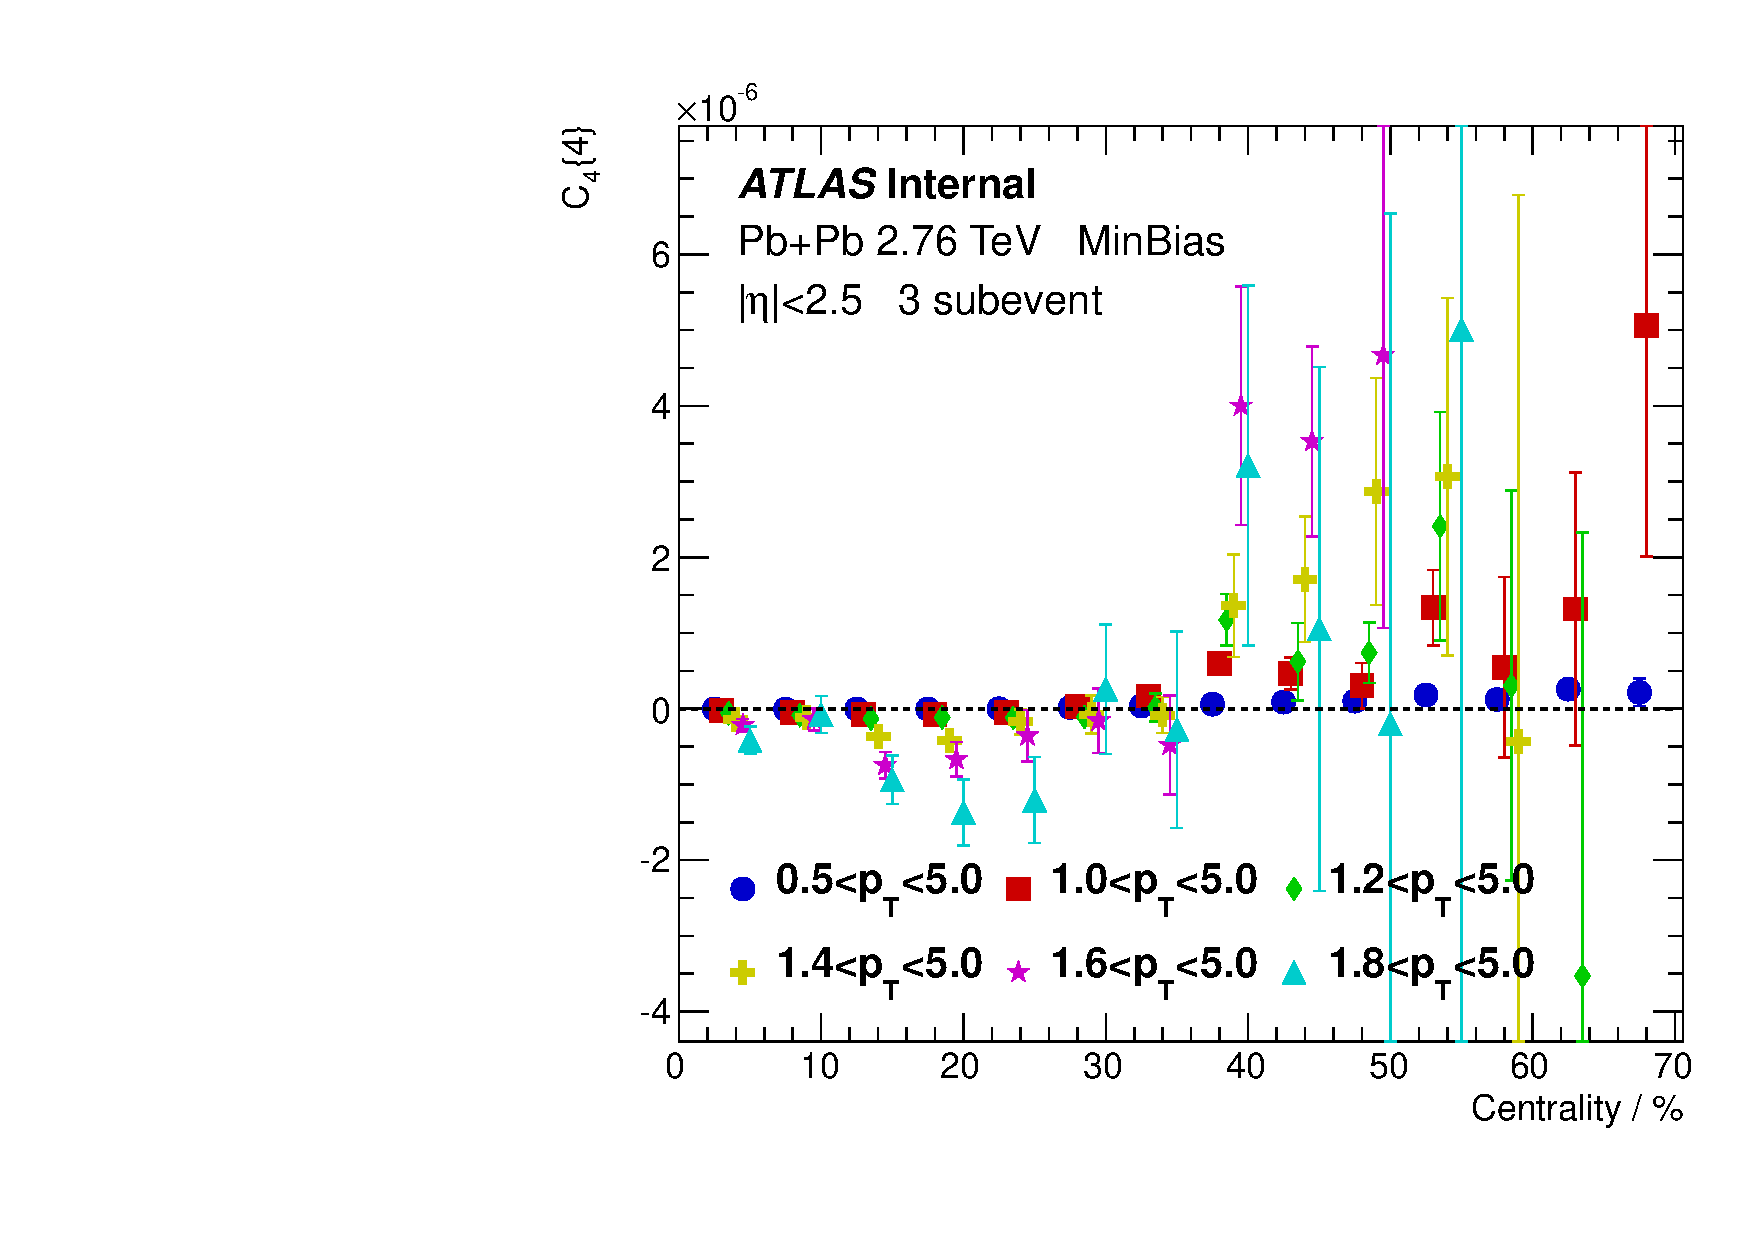
\includegraphics[width=.245\linewidth]{figs/sec_appendix/PbPb276/PbPb276_pT_3sub_Har4.pdf}
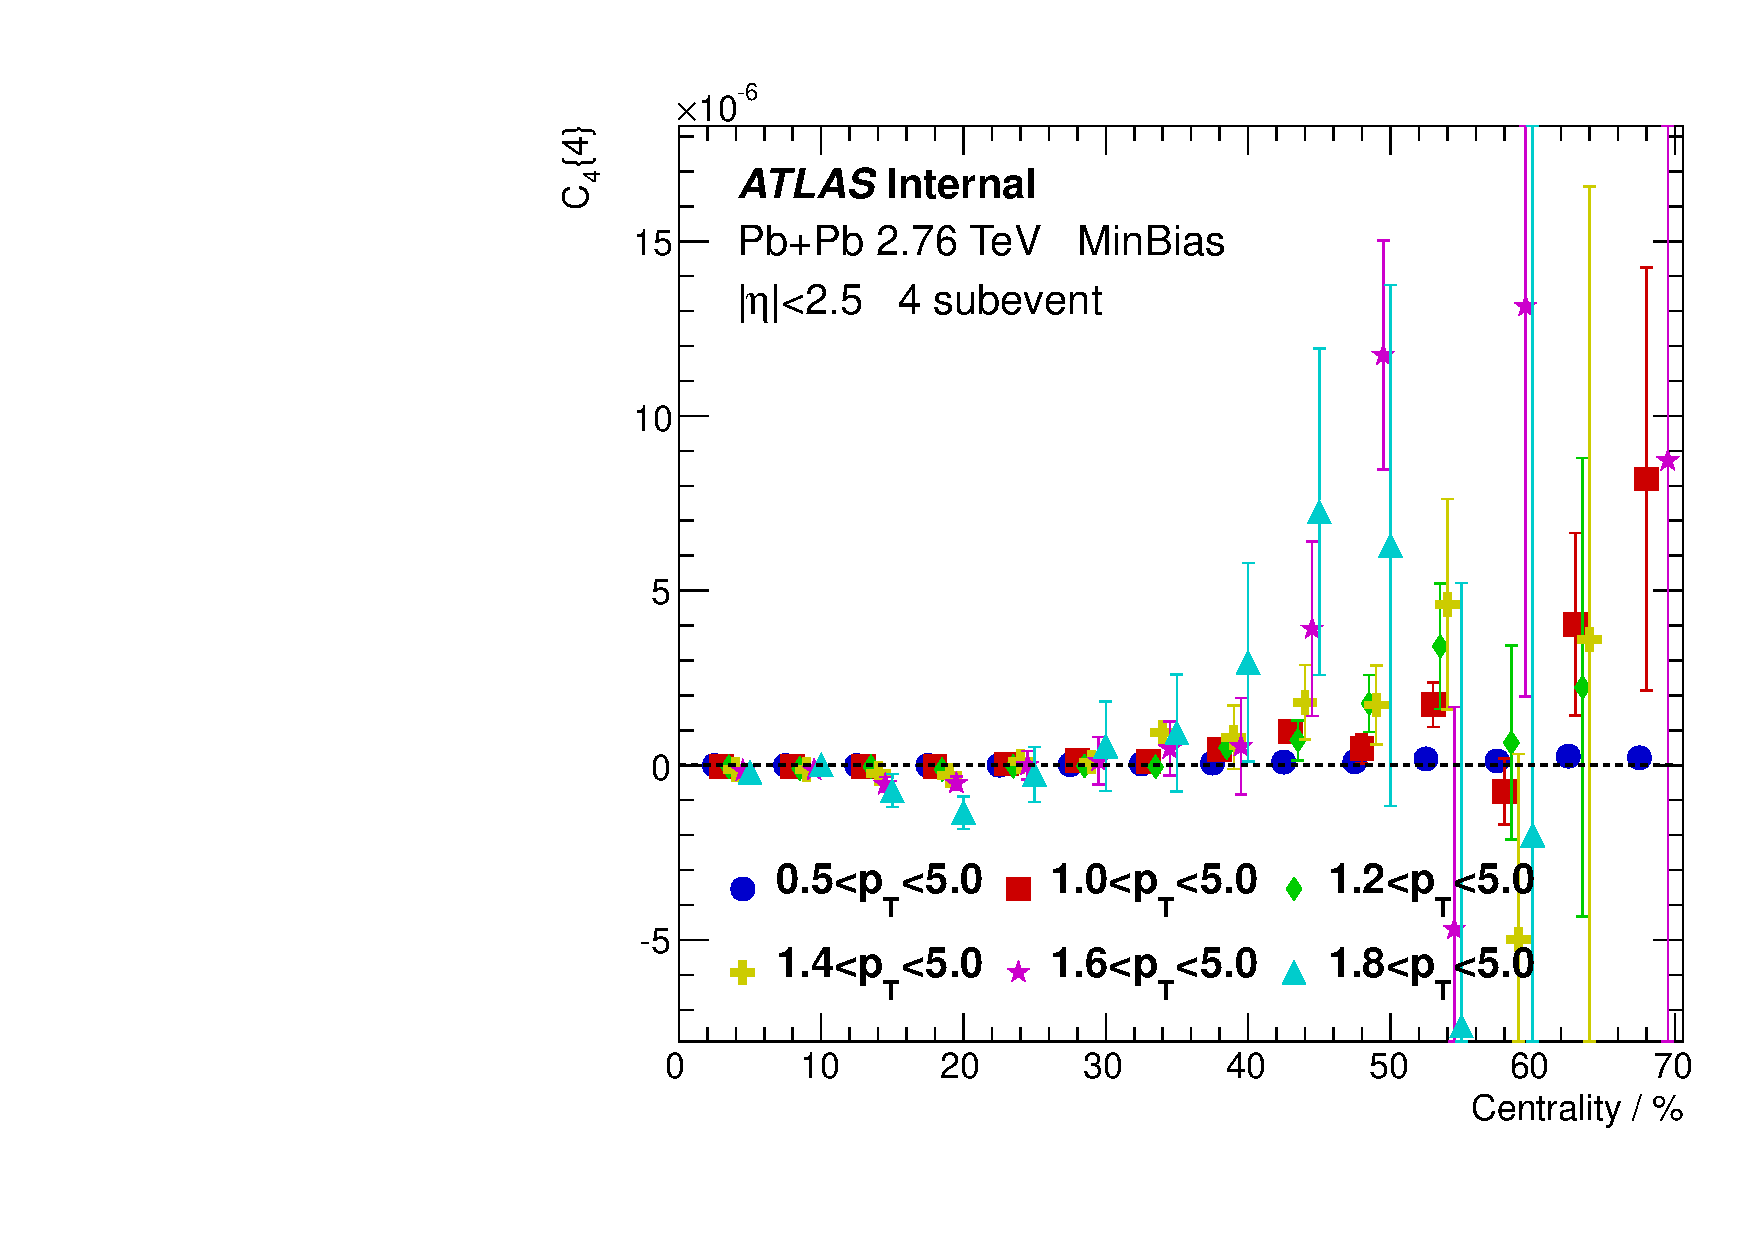
\includegraphics[width=.245\linewidth]{figs/sec_appendix/PbPb276/PbPb276_pT_4sub_Har4.pdf}
\caption{$c_4\{4\}$ in 2.76 TeV Pb+Pb, calculated in different $p_\text{T}$ ranges. Each panel is for each cumulant method.}
\label{fig:PbPb276_pT_v4}
\end{figure}

\begin{figure}[H]
\centering
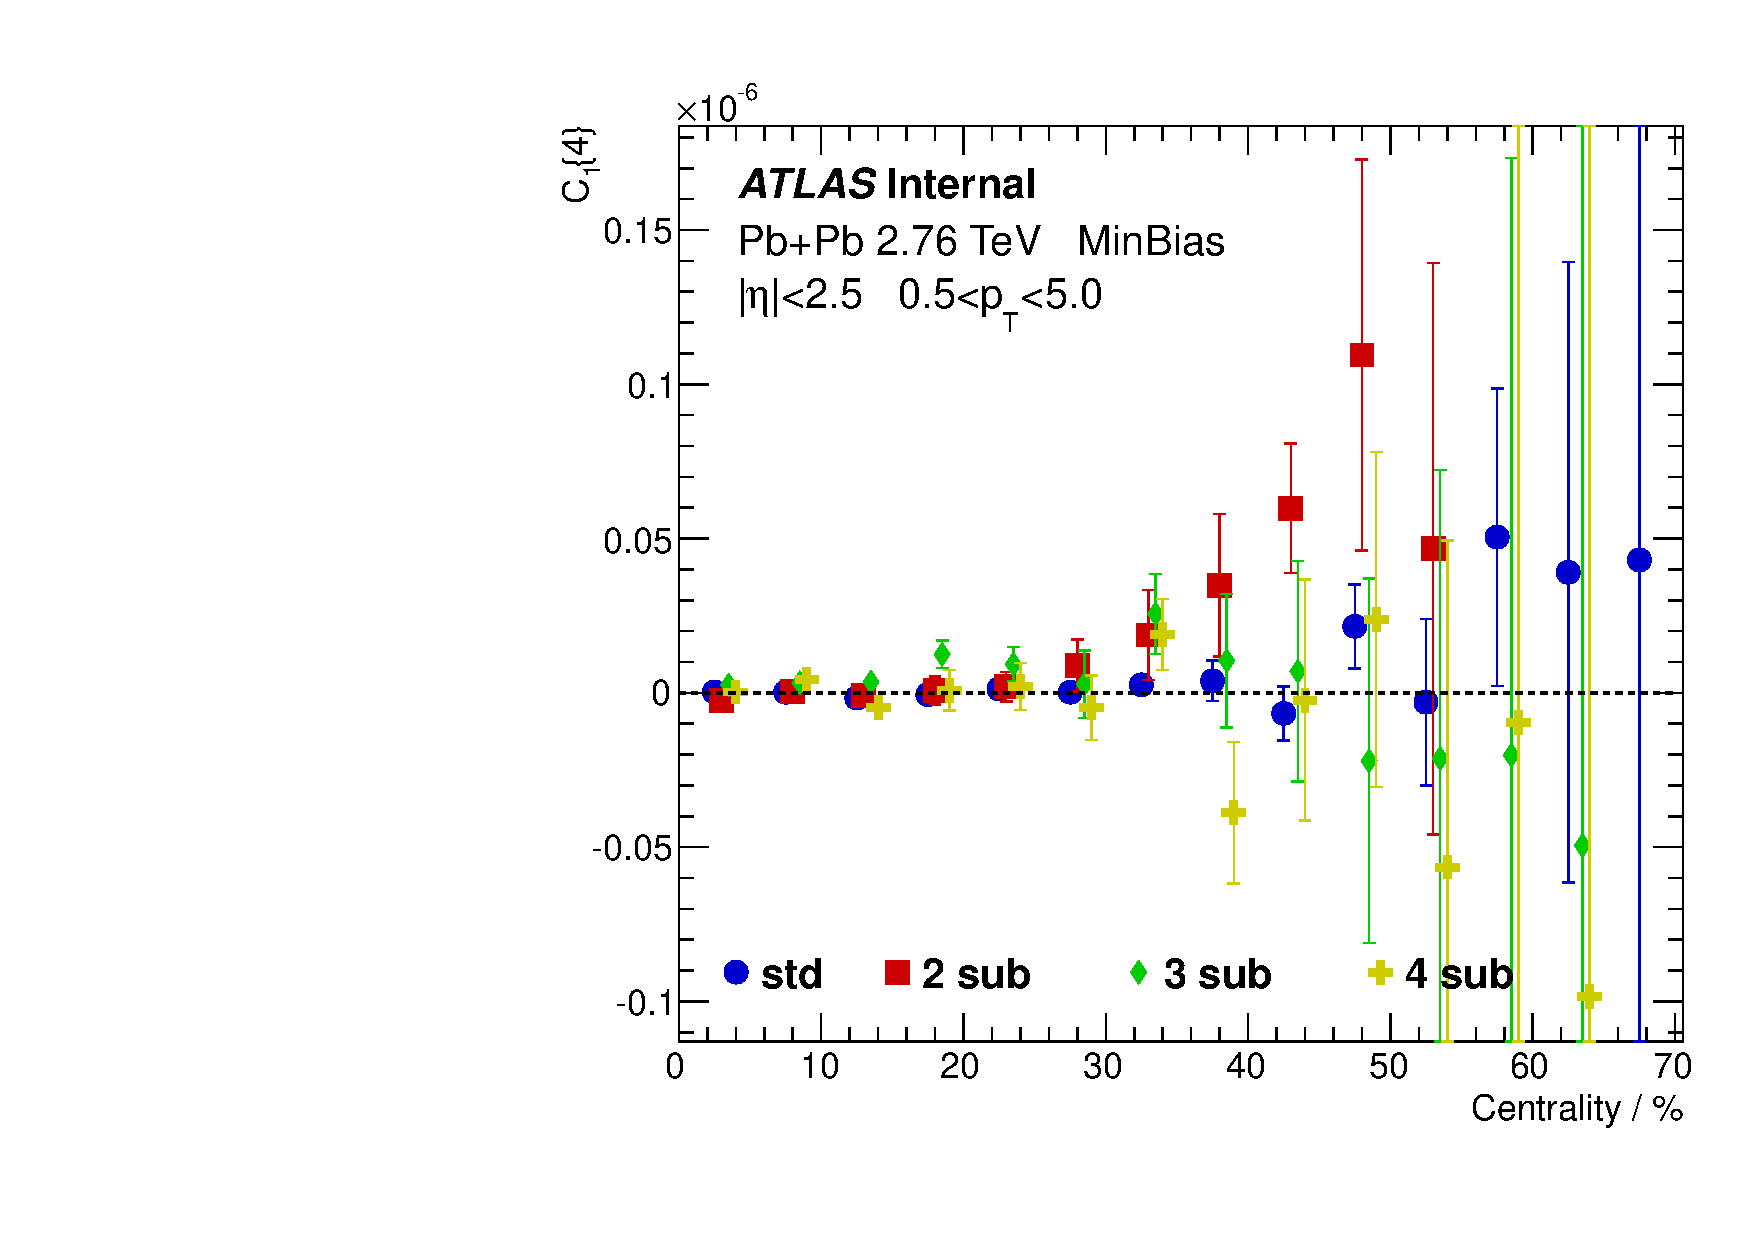
\includegraphics[width=.245\linewidth]{figs/sec_appendix/PbPb276/PbPb276_mtd_Har1_Pt0.pdf}
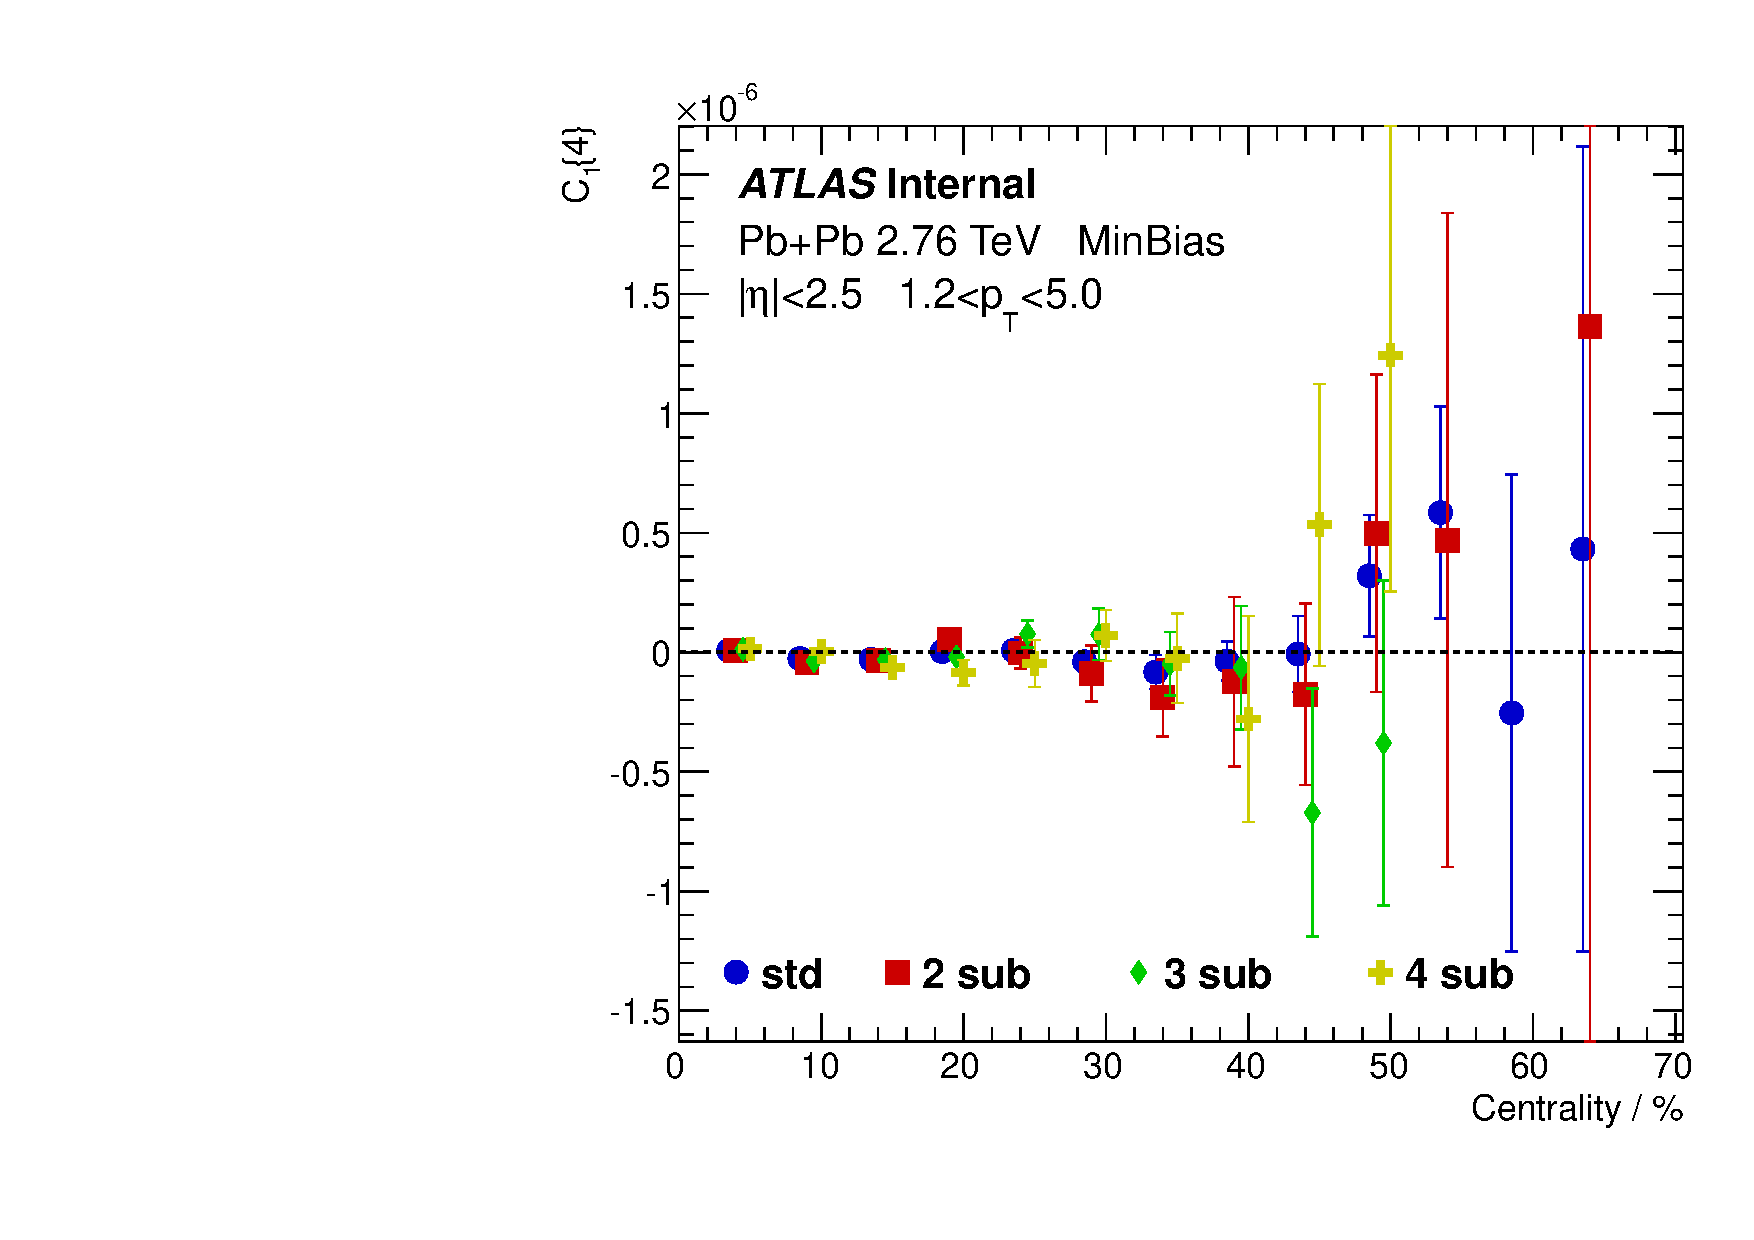
\includegraphics[width=.245\linewidth]{figs/sec_appendix/PbPb276/PbPb276_mtd_Har1_Pt2.pdf}
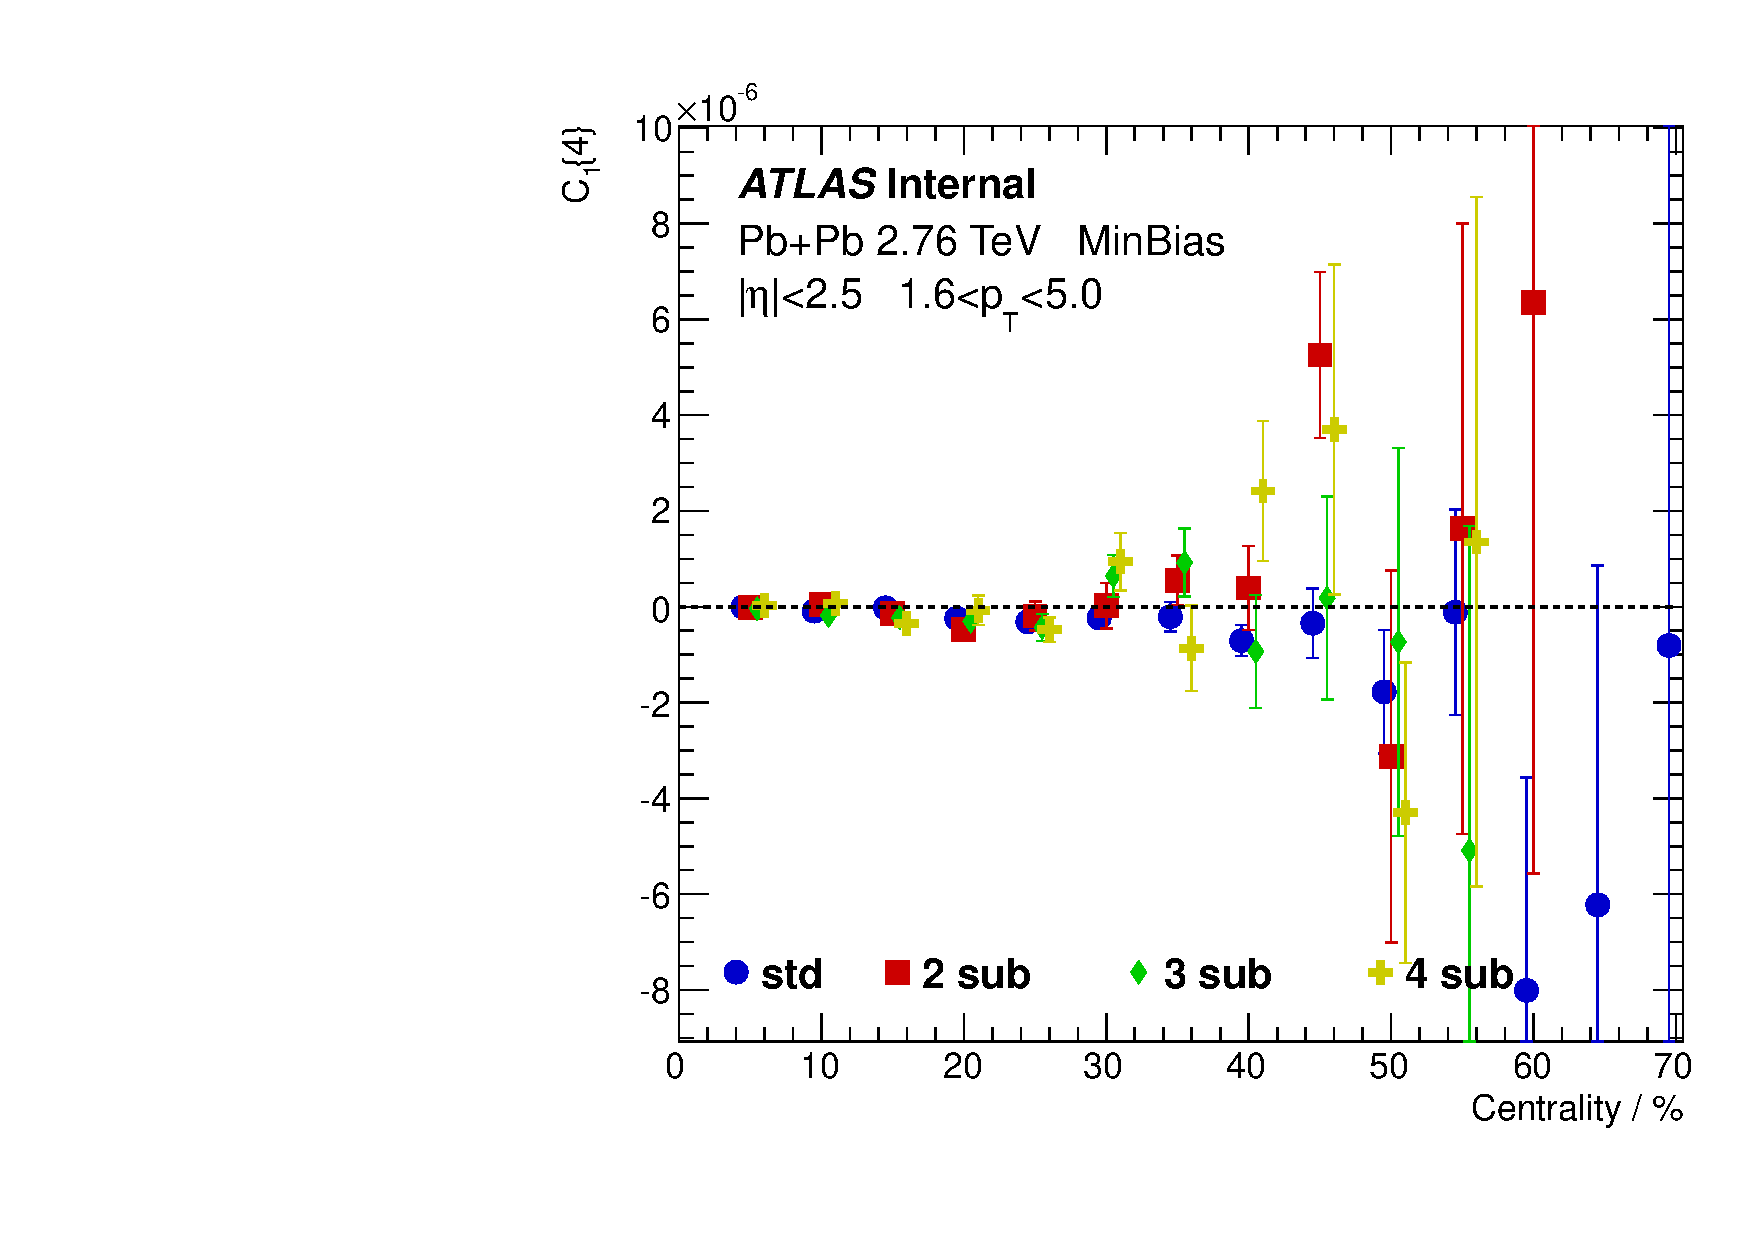
\includegraphics[width=.245\linewidth]{figs/sec_appendix/PbPb276/PbPb276_mtd_Har1_Pt4.pdf}
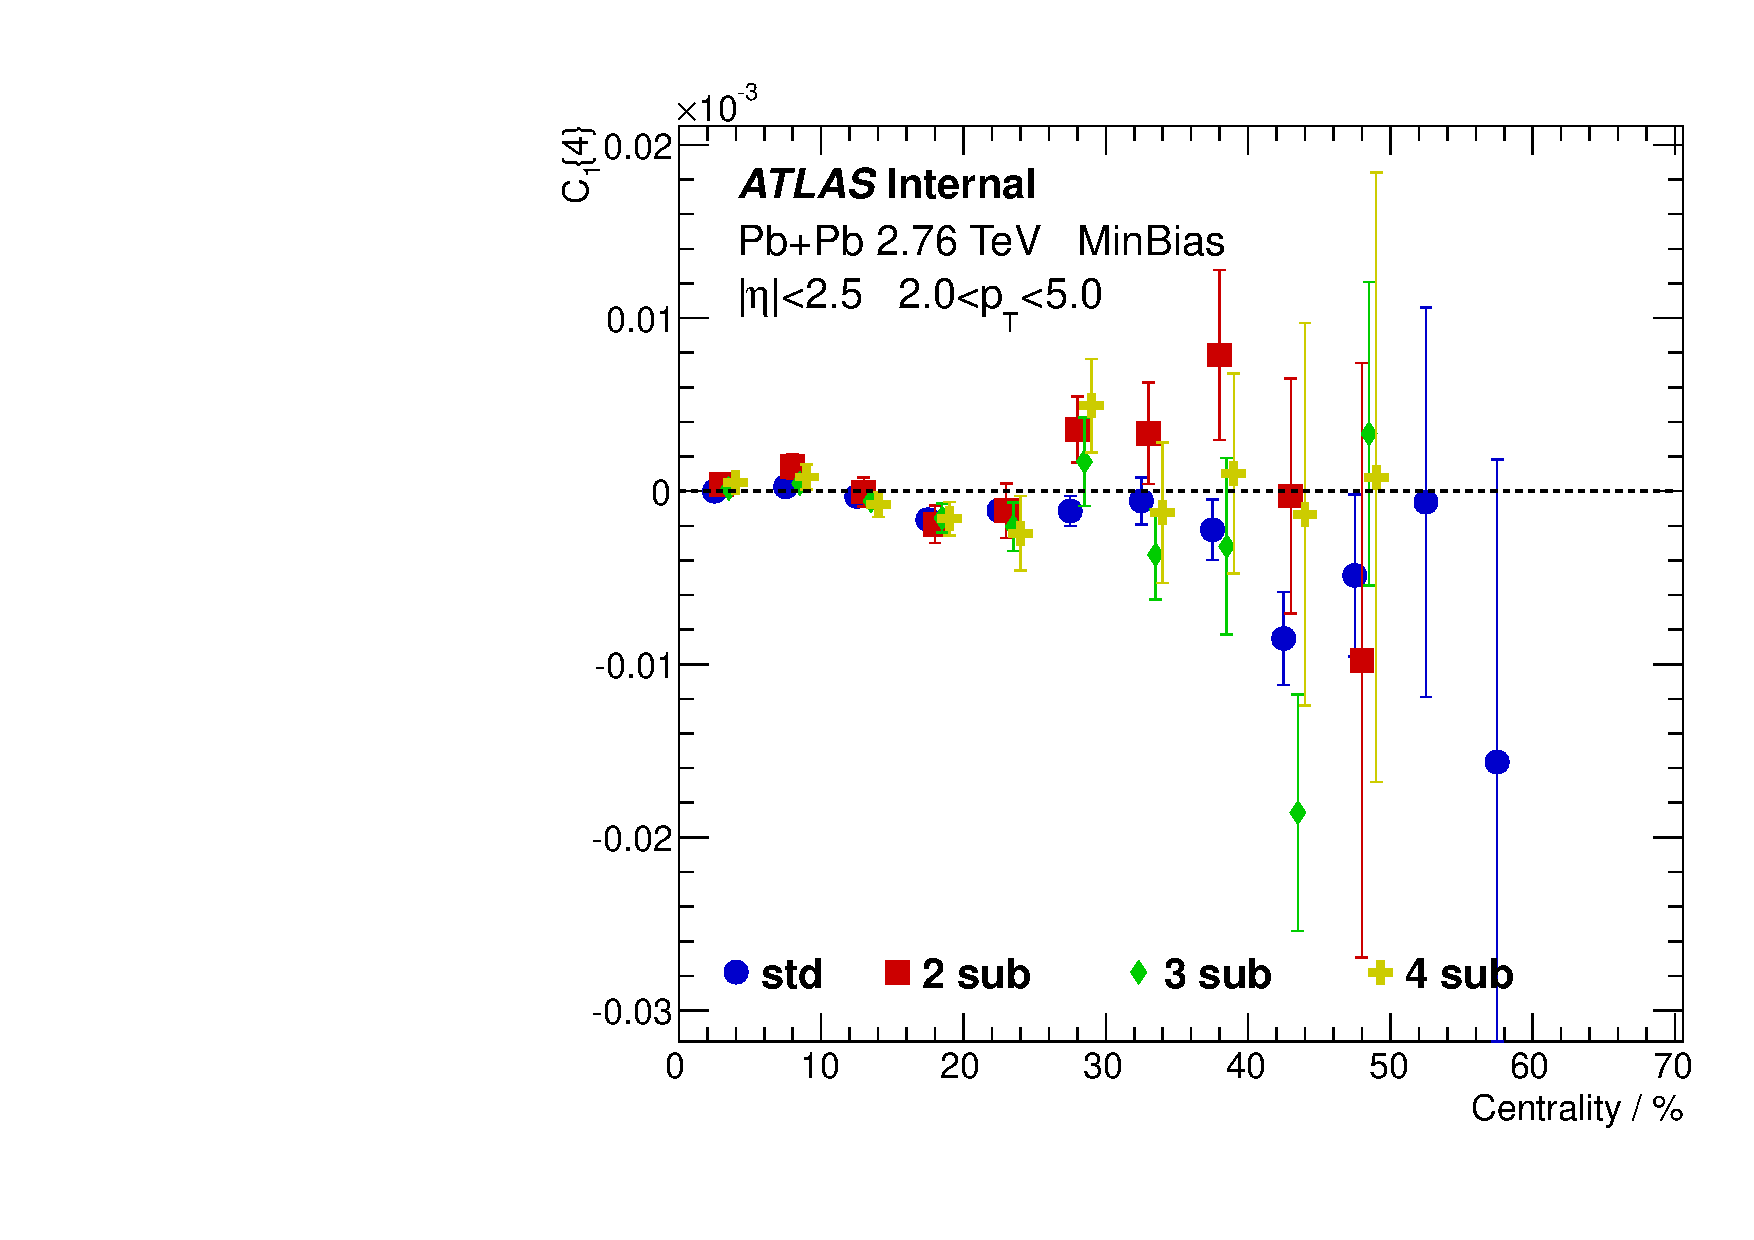
\includegraphics[width=.245\linewidth]{figs/sec_appendix/PbPb276/PbPb276_mtd_Har1_Pt6.pdf}
\caption{$c_1\{4\}$ in 2.76 TeV Pb+Pb, calculated with different cumulant methods. Each panel is for each $p_\text{T}$ range.}
\label{fig:PbPb276_mtd_v1}
\end{figure}

\begin{figure}[H]
\centering
\includegraphics[width=.245\linewidth]{figs/sec_appendix/PbPb276/PbPb276_mtd_Har2_Pt0.pdf}
\includegraphics[width=.245\linewidth]{figs/sec_appendix/PbPb276/PbPb276_mtd_Har2_Pt2.pdf}
\includegraphics[width=.245\linewidth]{figs/sec_appendix/PbPb276/PbPb276_mtd_Har2_Pt4.pdf}
\includegraphics[width=.245\linewidth]{figs/sec_appendix/PbPb276/PbPb276_mtd_Har2_Pt6.pdf}
\caption{$c_2\{4\}$ in 2.76 TeV Pb+Pb, calculated with different cumulant methods. Each panel is for each $p_\text{T}$ range.}
\label{fig:PbPb276_mtd_v2}
\end{figure}

\begin{figure}[H]
\centering
\includegraphics[width=.245\linewidth]{figs/sec_appendix/PbPb276/PbPb276_mtd_Har3_Pt0.pdf}
\includegraphics[width=.245\linewidth]{figs/sec_appendix/PbPb276/PbPb276_mtd_Har3_Pt2.pdf}
\includegraphics[width=.245\linewidth]{figs/sec_appendix/PbPb276/PbPb276_mtd_Har3_Pt4.pdf}
\includegraphics[width=.245\linewidth]{figs/sec_appendix/PbPb276/PbPb276_mtd_Har3_Pt6.pdf}
\caption{$c_3\{4\}$ in 2.76 TeV Pb+Pb, calculated with different cumulant methods. Each panel is for each $p_\text{T}$ range.}
\label{fig:PbPb276_mtd_v3}
\end{figure}

\begin{figure}[H]
\centering
\includegraphics[width=.245\linewidth]{figs/sec_appendix/PbPb276/PbPb276_mtd_Har4_Pt0.pdf}
\includegraphics[width=.245\linewidth]{figs/sec_appendix/PbPb276/PbPb276_mtd_Har4_Pt2.pdf}
\includegraphics[width=.245\linewidth]{figs/sec_appendix/PbPb276/PbPb276_mtd_Har4_Pt4.pdf}
\includegraphics[width=.245\linewidth]{figs/sec_appendix/PbPb276/PbPb276_mtd_Har4_Pt6.pdf}
\caption{$c_4\{4\}$ in 2.76 TeV Pb+Pb, calculated with different cumulant methods. Each panel is for each $p_\text{T}$ range.}
\label{fig:PbPb276_mtd_v4}
\end{figure}





\subsection{Results for 2.76 TeV Pb+Pb HIJING}

\begin{figure}[H]
\centering
\includegraphics[width=.45\linewidth]{figs/sec_appendix/HIJING_PbPb276/HIJING_PbPb276_pT_1sub_Har1.pdf}
\caption{$c_1\{4\}$ in 2.76 TeV HIJING Pb+Pb, calculated in different $p_\text{T}$ ranges.}
\label{fig:HIJING_PbPb276_pT_v1}
\end{figure}

